\documentclass[12pt,a4paper,twoside]{ipb}

% comentar caso seja uma disseração de mestrado
%\usepackage{projei}
\usepackage{csquotes} 
\usepackage[english]{babel}
\graphicspath{{./images/}}
\usepackage{listings} % incluir listagens
\usepackage{url} % typeset URL's
\usepackage[colorlinks=true,
                    urlcolor=black, %blue
                    linkcolor=black,
                    citecolor=black, %cor das citações
                    bookmarks=true,
                    pdfstartview=FitH]{hyperref}

% Pode ser usado biblatex
\usepackage[style=ieee,backend=biber]{biblatex}
\addbibresource{lib/refs.bib}
\usepackage{pgffor}

\usepackage{hyperref}

\usepackage{lipsum}

\usepackage{amsmath}

\usepackage{tabulary}

\usepackage{booktabs}

\usepackage{graphicx}

\usepackage{layout}

\usepackage[table]{xcolor}

\usepackage{subcaption}

\usepackage{array}

\usepackage{multirow}

\usepackage{soul}

\usepackage{eurosym}

\usepackage{amsfonts}

\usepackage{listings}

\usepackage{float}

%\usepackage[newfloat]{minted}
\usepackage[outputdir=/home/iaggo/anaconda3/bin/pygmentize/]{minted}

\usepackage{appendix}

% Add this command to define the problematic character
\DeclareUnicodeCharacter{0301}{\'{e}} % Replace 0301 with the Unicode code of the character causing the error


\definecolor{jsongray}{RGB}{100,100,100}
\definecolor{jsonlightgray}{RGB}{200,200,200}
\definecolor{darkgray}{RGB}{33,47,60}
\definecolor{jsonpurple}{RGB}{128,0,128}


\definecolor{keywordcolor}{rgb}{0.85, 0.49, 0.19} % Orange for packages (like "logger")
\definecolor{keywordcolor2}{rgb}{1, 0.372, 0.12} % Blue for info
\definecolor{keywordcolor3}{rgb}{0, 0.06, 0.93} % Blue for info
\definecolor{stringcolor}{rgb}{0.33, 0.33, 0.33}  % Dark Gray for strings
\definecolor{commentcolor}{rgb}{0.07, 0.549, 0.29}    % Green for comments
\definecolor{numbercolor}{rgb}{0.39, 0.56, 0.86}  % Blue for numbers
\definecolor{codegray}{rgb}{0.5,0.5,0.5}
\definecolor{backcolour}{rgb}{1,1,1} % White for background

\lstdefinestyle{VSCode}{
    language=Python,
    basicstyle=\ttfamily\small,
    keywordstyle=[1]\color{keywordcolor},
    keywordstyle=[2]\color{keywordcolor2},
    keywordstyle=[3]\color{keywordcolor3},
    stringstyle=\color{stringcolor},
    commentstyle=\color{commentcolor},
    numberstyle=\color{numbercolor},
    tabsize=2,
    showstringspaces=false,
    backgroundcolor=\color{backcolour},
    rulecolor=\color{backcolour},
    frame=single, 
    rulecolor=\color{codegray},
    showspaces=false,
    showtabs=false, 
    breaklines=true,
    postbreak=\mbox{\textcolor{codegray}{$\hookrightarrow$}\space},
    morekeywords=[2]{logger, cv, numpy, settings, }  % Defining "info" as a keyword
    morekeywords=[3]{canny_frame, dilatation, dilated_frame, eroded_frame, contours, ratio, clean_contour_points, contour, contours, bbox, show_frame}
}

\lstdefinelanguage{Python}{
  keywords={and, as, assert, break, class, continue, def, del, elif, else, except, exec, finally, for, from, global, if, import, in, is, lambda, not, or, pass, print, raise, return, try, while, with, yield, None, True, False, bool, int, float, str, list},
  comment=[l]{\#},
  string=[b]{'''},
  string=[b]{"""}
  string=[b]{'},
  string=[b]{"},
  showstringspaces=false
}
\usepackage{color}
\definecolor{keywordcolor}{rgb}{0.58,0,0.82}
\definecolor{stringcolor}{rgb}{0.67,0.33,0}
\definecolor{commentcolor}{rgb}{0.33,0.33,0.33}
\definecolor{numbercolor}{rgb}{0,0,1.0}
\definecolor{pygreen}{rgb}{0.0,0.5,0.0}

\lstdefinestyle{pycharm}{
    language=Python,
    basicstyle=\ttfamily\small,
    keywordstyle=\color{keywordcolor}\bfseries,
    stringstyle=\color{stringcolor},
    commentstyle=\color{commentcolor},
    numberstyle=\color{numbercolor},
    showstringspaces=false,
    identifierstyle=\color{black},
    tabsize=2,
    emph={self}, emphstyle=\color{pygreen},
    literate=*{:}{{\textcolor{keywordcolor}{:}}}{1}%
             {=}{{\textcolor{keywordcolor}{=}}}{1}%
             {-}{{\textcolor{keywordcolor}{-}}}{1}%
             {+}{{\textcolor{keywordcolor}{+}}}{1}%
             {*}{{\textcolor{keywordcolor}{*}}}{1}%
             {!}{{\textcolor{keywordcolor}{!}}}{1}%
             {(}{{\textcolor{keywordcolor}{(}}}{1}%
             {)}{{\textcolor{keywordcolor}{)}}}{1}%
             {[}{{\textcolor{keywordcolor}{[}}}{1}%
             {]}{{\textcolor{keywordcolor}{]}}}{1}%
             {<}{{\textcolor{keywordcolor}{<}}}{1}%
             {>}{{\textcolor{keywordcolor}{>}}}{1}%
             {/}{{\textcolor{keywordcolor}{/}}}{1}%
             {^}{{\textcolor{keywordcolor}{^}}}{1}%
             {&}{{\textcolor{keywordcolor}{&}}}{1}%
             {~}{{\textcolor{keywordcolor}{~}}}{1}%
             {.}{{\textcolor{keywordcolor}{.}}}{1}%
}

\lstdefinelanguage{yaml}{
  keywords={true,false,null,y,n},
  keywordstyle=\color{darkgreen},
  basicstyle=\ttfamily\small,
  sensitive=false,
  comment=[l]{\#},
  morecomment=[s]{/*}{*/},
  commentstyle=\color{purple}\ttfamily,
  stringstyle=\color{red}\ttfamily,
  showstringspaces=false,
  identifierstyle=\color{blue},
  morestring=[b]',
  morestring=[b]"
}
\lstdefinelanguage{json}{
    basicstyle=\ttfamily\small\color{jsonlightgray},
    columns=fullflexible,
    showstringspaces=false,
    commentstyle=\color{gray}\upshape,
    keywordstyle=\color{jsongray}\bfseries,
    stringstyle=\color{jsonpurple},
    breakatwhitespace=true,
    morestring=[b]",
    morecomment=[l]{//},
    morecomment=[s]{/*}{*/},
    morekeywords={true,false,null},
    breaklines=true, % Wrap lines within the frame
}

\lstset{
    language=json,
    frame=single,
    numbers=left,
    numberstyle=\scriptsize\color{gray},
    stepnumber=1,
    numbersep=5pt,
    captionpos=b,
    tabsize=2,
    xleftmargin=15pt,
    xrightmargin=15pt,
    framexleftmargin=15pt,
    framextopmargin=5pt,
    framexbottommargin=5pt,
    showspaces=false,
    showtabs=false,
    showstringspaces=false,
    breaklines=true,
}

\lstdefinestyle{linux}{
    backgroundcolor=\color{white},
    basicstyle=\color{darkgray!70!black}\small\bfseries,
    keywordstyle=\color{blue!70!black}\bfseries,
    commentstyle=\color{gray}\itshape,
    stringstyle=\color{darkgray},
    frame=single,
    framexleftmargin=15pt,
    framexrightmargin=15pt,
    framextopmargin=5pt,
    framexbottommargin=5pt,
    rulecolor=\color{jsonlightgray}, % Set frame color to dark gray
    showstringspaces=false,
    xleftmargin=15pt,
    xrightmargin=5pt,
    stepnumber=1,
    numbersep=5pt,
    captionpos=b,
    numbers=left,
    numberstyle=\scriptsize\color{gray},
    breaklines=true, % Wrap lines within the frame
}


\lstdefinestyle{nginx}{
    basicstyle=\color{gray!70!black}\small\ttfamily,
    keywordstyle=\color{blue!70!black}\bfseries,
    commentstyle=\color{gray!60}\bfseries,
    stringstyle=\color{white},
    morekeywords={server, location, root, index},
    breaklines=true,
    showstringspaces=false,
}

% Create a new environment for Nginx configuration listing


% Define the Nginx language
\lstdefinelanguage{nginx}{
    keywords={worker_processes, http, upstream, server, listen, location, proxy_pass, proxy_set_header, proxy_read_timeout, proxy_send_timeout},
    keywordstyle=\bfseries\color{blue},
    morestring=[b]",
    morecomment=[l]{\#},
}

%\title{Desenvolvimento de um Sistema de Monitorização para Reservatórios para a Santa Casa da Misericórdia de Bragança}

%%\title{Development of an Integrated System for Industrial Laundry at Santa Casa da Misericórdia de Bragança}

%%(jpc)\title{IoT system applied to detergent supervision in industrial washing machines}

\title{\textbf{Development of Traceability Solution for Furniture Components}}

\author{Iaggo Capitanio - 52498}
%\authnum{1}
%\secondauthor{Nome do Aluno - Número Mecanográfico}
%\secauthnum{2}

\supervisor{Prof. Dr. João Paulo Coelho}
\cosupervisor{Prof. Dr. Luan José Franchini Ferreira }
\cosupervisor{Filipe Mofreita, Carpintaria Mofreita}
\cosupervisor{Prof. José Alexandre de Carvalho Gonçalves}
\cosupervisors{
    Prof. Dr. Luan José Franchini Ferreira,
    Filipe Mofreita - Carpintaria Mofreita,
    Prof. Dr. José Alexandre de Carvalho Gonçalves
}

% Para definir o ano letivo
\courseyear{2023}

% Para nao mostrar a lista de tabelas
%\tablespagefalse

\makeglossaries
\loadglsentries{acronym}
\loadglsentries{glossary}



%http://tex.stackexchange.com/questions/59572/custom-page-numbering-for-appendix
\usepackage{etoolbox}
\usepackage{verbatim}

\begin{document}
	
% Coloca a capa, primeira pagina e outros

\beforepreface

%\cleardoublepage

\prefacesection{Dedication}
%\thispagestyle{empty}

%\lipsum[1]

I would like to dedicate this work to my parents, Ana Maria Capitanio and Flavio Capitanio. It is thanks to their unwavering support and encouragement that my dream of studying abroad became a reality. Their love, guidance, and sacrifices have been instrumental in shaping my academic journey, and I am deeply grateful for their constant belief in me. This accomplishment would not have been possible without them, and I am forever thankful for their presence in my life.

%\vfill
%\pagebreak
%\mbox{}
%\vfill
%\pagebreak

%\cleardoublepage

\prefacesection{Acknowledgment}
%\thispagestyle{empty}

%\lipsum[1]

I would like to express my deep gratitude to all the people who were present at this important stage of my life and who contributed to the realization of this work. Even those whom I may never have met personally played a key role in the structure that made this project possible.

First of all, I would like to express my sincere gratitude to my beloved family for their unconditional support throughout this journey. In particular, I would like to thank my mother, Ana Maria Capitanio, and my father, Flavio Capitanio, for being a constant source of love and encouragement. I am also grateful to my sister, Raissa Capitanio, for her continued support and encouragement.

In addition, my deepest gratitude extends to my wife, Debora de Lima Wahlus, for her unwavering support and for being by my side throughout the process. Her presence and support have been invaluable.

A special thanks goes to my supervisor, João Paulo Coelho, for giving me the opportunity to do this amazing work. His guidance, knowledge, and incentive were fundamental for the success of this project. I am also grateful to my advisor in Brazil, Juan José Franchini Ferreira, for his constant support and sharing of knowledge.

I would like to express my gratitude to Professor Christian Naaktgeboren, for sharing his knowledge during my studies and being an inspiration as an academic and engineer.

To my home university, the Universidade Tecnológica Federal do Paraná, I express my gratitude for offering me a free and quality education with excellent teachers. Furthermore, I am grateful for the opportunity to participate in the Dual Diplomacy program, which allowed me to expand my academic and cultural horizons.

I would also like to thank my friend Carlos Seiti for his constant support and motivational talks. His quest for personal growth and constant improvement inspires me.

Finally, I would like to express my gratitude to Instituto Politécnico de Bragança for welcoming me to Portugal and to the partner company More, especially Nuno Manuel Pereira Guedes, for their valuable contribution to this project. His collaboration and support were fundamental for the success of this work.

%\vfill
%\pagebreak
%\mbox{}
%\vfill
%\pagebreak


%\cleardoublepage

\prefacesection{Abstract}
%\thispagestyle{empty}


In the contemporary context, characterized by intensified global competition and the constant evolution of the globalization landscape, it becomes imperative for industries, including Small and Medium Enterprises (SMEs), to undertake efforts to enhance their operational processes, often through digital technological adaptation. The present study falls within the scope of the project named “Wood Work 4.0,” which aims to infuse innovation into the wood furniture manufacturing industry through process optimization and the adoption of digital technologies. This project received funding from the European Union Development Fund, in collaboration with the North 2020 Regional Program, and was carried out at the Carpintaria Mofreita company, located in Macedo de Cavaleiros, Portugal. In this regard, this study introduces a software architecture that supports the traceability of projects in the wood furniture industry and simultaneously employs a system to identify and manage material leftovers, aiming for more efficient waste management. For the development of this software architecture, an approach that integrates the Fiware platform, specialized in systems for the Internet of Things (IoT), with an Application Programming Interface (API) specifically created to manage information about users, projects, and associated media files, was adopted. The material leftovers identification system employs image processing techniques to extract geometric characteristics of the materials. Additionally, these data are integrated into the company’s database. In this way, it was possible to develop an architecture that allows not only the capturing of project information but also its effective management. In the case of material leftovers identification, the system was able to establish, with a satisfactory degree of accuracy, the dimensions of the materials, enabling the insertion of these data into the company's database for resource management and optimization.

\bigskip

\noindent \textbf{Keywords:} Wood Work 4.0 Project; Internet of Things ; Image Processing; Industrial Digitalization.



%\cleardoublepage

\prefacesection{Resumo}
%\thispagestyle{empty}


No contexto contemporâneo, marcado por uma competição global intensificada e pela constante evolução do cenário de globalização, torna-se imperativo para as indústrias, incluindo as Pequenas e Médias Empresas (PMEs), empreender esforços para aprimorar seus processos operacionais, frequentemente pela via da adaptação tecnológica digital. O presente estudo insere-se dentro do escopo do projeto denominado “Wood Work 4.0”, cujo propósito é infundir inovação na indústria de fabricação de móveis de madeira por meio da otimização de processos e da adoção de tecnologias digitais. Este projeto obteve financiamento do Fundo de Desenvolvimento da União Europeia, em colaboração com o programa Regional do Norte 2020 e foi realizado na empresa Carpintaria Mofreita, localizada em Macedo de Cavaleiros, Portugal. Nesse sentido, este estudo introduz uma arquitetura de software que oferece suporte à rastreabilidade de projetos na indústria de móveis de madeira, e simultaneamente emprega um sistema para identificar e gerenciar sobras de material, objetivando uma gestão de resíduos mais eficiente. Para o desenvolvimento dessa arquitetura de software, adotou-se uma abordagem que integra a plataforma Fiware, especializada em sistemas para a Internet das Coisas (IoT), com uma Interface de Programação de Aplicações (API) criada especificamente para gerenciar informações de usuários, projetos, e arquivos de mídia associados. O sistema de identificação de sobras de material emprega técnicas de processamento de imagem para extrair características geométricas dos materiais. Adicionalmente, esses dados são integrados ao banco de dados da empresa. Desta forma, foi possível desenvolver uma arquitetura que permite não só capturar informações de projetos, mas também gerenciá-las de forma eficaz. No caso da identificação de sobras de material, o sistema foi capaz de estabelecer, com um grau de precisão satisfatório, as dimensões dos materiais, possibilitando a inserção desses dados no banco de dados da empresa para gestão e otimização do uso de recursos.

\bigskip

\noindent \textbf{Palavras-chave:} Projeto Wood Work 4.0 ;  Internet das Coisas; Processamento de Imagem; Digitalização Industrial.


% Coloca indices
\afterpreface

\printglossary[type=\acronymtype,nonumberlist,title={List of Acronyms}]

\newpage

\bodystart

% Capitulos do documento
\cleardoublepage
\chapter{Introduction}\label{cap:intro}

This thesis is directly correlated with the context of the Wood Work 4.0 project, funded by the European Union's Regional Development Fund in conjunction with the NORTE 2020 regional investment program and promoted by Mofreita Industries. The case study in this research is conducted at Mofreita Industries, a company engaged in the production of furniture in the wood industry sector.

In this company, despite significant advancements in modern machinery, the operational processes are still carried out in an outdated manner. Many project management and tracking operations are performed using paper-based methods and other outdated techniques, negatively impacting the efficiency of the system. Hence, the primary objective of this project is to foster enhanced digitalization within the wood industry, specifically focusing on the domain of furniture manufacturing.

Furthermore, the wood furniture manufacturing industry faces a recurring challenge in effectively managing cut-offs or remnants. Two distinct categories of cut-offs exist: those suitable for reuse and those that lack any potential for re-purposing. The non-reusable cut-offs encompass damaged wooden pieces or those with significantly limited cutting areas. Conversely, reusable cut-offs possess ample usable space. Unfortunately, these reusable remnants are not adequately documented or cataloged; instead, they are haphazardly stacked within storage areas, devoid of any systematic inventory management practices. This inadequacy gives rise to two significant complications: first, the inefficient utilization of available pieces, as workers may opt to use larger wood sections instead of selecting more suitable alternatives, and second, the wastage of valuable human resources and time spent on the laborious task of searching for an appropriate piece to fulfill specific project requirements.

Indeed, in the contemporary business scenario, there is a relentless effort by companies to optimize their production processes through the use of new technologies \cite{JewapatarakulDigitalTransformation, DingEffectsofIoT, GUNTHER2017191}. The declining competitiveness of the industrial sector in European countries has led to the adoption of an industrial strategy driven by the use of technologies such as robotics, sensors, Big Data, machine learning, and telecommunication networks between devices \cite{HerreroMeasuringTheEffectivenessOfIndustrialProcesses}. This new approach to industrialization, encouraged by the European Union (EU) countries, aims to improve the utilization of natural resources and increase the competitiveness of industries. This approach uses a deeper integration of the manufacturing processes, with technologies that allow rapid sharing of data between production processes. In this way, value and information can be added to the production chain, increasing competitiveness\cite{Grabowska+2020+90+96}.

This new paradigm implies a broader digitization of the industry, transcending simple management and resulting in the creation of \emph{"smart products"} that are integrated into the value chain and are part of the company's virtual environment. This allows tracking the location of these products in the manufacturing environment, identification of the production process they are in, and provision of information to customers about the status of their orders \cite{economies6030046}. These possibilities contribute to the improvement of competitiveness and the integration of processes \cite{SeungSME}.

Building upon these advancements, the main idea of Industry 4.0 is to create a corporate network that allows data exchange between intelligent components capable of communicating with each other \cite{Grabowska+2020+90+96}. In this context, we highlight the \acrfull{iiot}\footnote{Industrial Internet of Things is a computing concept that describes communication between devices and services on an enterprise network \cite{Sisinni8401919}.}, a technology model that fits perfectly in this  of data sharing dynamics \cite{GARG2022286}.


\acrfull{iiot}, a technology that enables task and process automation, operates through a \acrfull{m2m} type communication. This form of communication is characterized by the exchange of data between devices and services, without the need for human intervention. This process is enabled by the use of sensors, \acrfull{rfid} tags, network services, and other devices that are connected to the Internet. These devices can not only communicate with each other, but also interact with devices external to the network\cite{KhanIoT}. Therefore, through \acrshort{m2m} communication, companies can automate tasks and processes, allowing devices and services to collect real-time data and make decisions autonomously and instantaneously. For example, \acrshort{m2m} communication can be used to monitor the location of parts in the production environment, and reporting productions delays and unusul events. In this way, it is possible to improve the effectiveness of the manufacturing process, reduce waste and costs \cite{SeungSME}. This technology also can help corporations improve the user experience, both for the end consumer and the product development team \cite{Grabowska+2020+90+96}.

From the end user's point of view, M2M communication can enable real-time tracking of the development status of their customized product. This is possible by collecting real-time data about the production process and making this data available to the customer via a portal or application. Such a practice can give the customer a clearer view of the progress of his order, thereby increasing his satisfaction with the service.

From the product development team's point of view, M2M communication can allow individuals to quickly obtain information about previous products with similar characteristics to the product being developed. This information can be gathered through attributes such as geometric information, material, lead time, and more. This can help the team better understand customer needs and preferences, and speed up the modeling process.

Building upon the advantages of \acrfull{it} in the industry, the adoption of IT-driven approaches brings forth a multitude of benefits. By harnessing IT solutions, companies can gain a comprehensive understanding of their manufacturing operations, thereby delving deeper into both the products themselves and the desires of their customers. As a result, IT-driven approaches positively impact the entire product value chain, encompassing critical aspects like design, production, distribution, and customer satisfaction \cite{economies6030046}. Through the integration of IT, businesses can optimize operational efficiency, streamline workflows, enhance quality control, facilitate data-driven decision-making, and foster innovation in their respective industries. These advancements collectively contribute to heightened competitiveness, improved customer experiences, and overall business success.

The implementation of Industry 4.0 technologies in the furniture industry is still little explored, making this study of paramount importance. The project "Development of Traceability Solution for Furniture Components" uses image processing methods in order to reduce process losses in the furniture industry, aligning with goal number 12 of the UN's SDGs (Sustainable Development Goals), which seeks to promote sustainable production and consumption patterns. This traceability solution allows the tracking and monitoring of components used in furniture manufacturing, contributing to the promotion of sustainability throughout the production chain. The combination of the implementation of SDG 12 with image processing techniques in this project exemplifies the innovative application of technology, driving sustainability in the furniture industry and contributing to a more responsible and conscious future.

The issue of digitization in small and medium-sized enterprises (SMEs), particularly those involved in the secondary sector of wood processing, is a pressing matter that requires attention. Among the initiatives aimed at addressing this challenge, the Wood Work 4.0 project stands out as a significant endeavor funded by the NORTE 2020 program and the European regional development fund. This project brings together various partners, each with their own objectives, to explore the implementation of Industry 4.0 technologies in the furniture industry.

This theses was developed in the context of the Wood Work 4.0 project. It recognizes the limited exploration of Industry 4.0 technologies in the furniture industry, highlighting the paramount importance of this study. By utilizing image processing methods, the project aims to minimize process losses within the furniture industry, aligning its objectives with goal number 12 of the UN's Sustainable Development Goals (SDGs). This goal focuses on promoting sustainable production and consumption patterns, a crucial aspect in today's world.

The traceability architecture solution developed in this project enables the tracking and monitoring of components used in furniture manufacturing, thereby contributing to the promotion of sustainability throughout the entire production chain. By combining the implementation of SDG 12 with innovative image processing techniques, this project exemplifies the forward-thinking application of technology in driving sustainability within the furniture industry. Ultimately, the Woodwork 4.0 project aspires to create a more responsible and conscious future by fostering sustainable practices and leveraging the potential of digitalization in \acrshort{smes} involved in wood processing.

By addressing this gap, this study has the potential to contribute to the development of the furniture manufacturing sector. It can identify opportunities for improvement, develop innovative solutions, and drive digital transformation in the sector. Furthermore, this study can provide insights into how Industry 4.0 can be translated to a particular case study. This is especially relevant in an increasingly competitive and constantly evolving market, where companies must continuously seek innovations to stand out \cite{ghobakhloo2021industry}.


\section{Motivation}\label{cap:intro:justification}

The motivation behind this work is to promote technological advances in the wooden furniture manufacturing industry, making it more competitive on the world stage. The proposal consists in apply advanced image processing techniques to improve the management of wood waste generated during the production process. Currently, these surplus materials are often mismanaged and underutilized.

Implementing a waste management program based on image processing has the potential  to significantly reduce costs, optimizing the use of this waste contributes to the preservation of the environment by avoiding waste of natural resources and minimizing the need to cut down new trees for wood production. This reflects a more sustainable and ecologically conscious approach. In addition to bringing a positive image to the company.

Therefore, the ultimate goal of this work is to provide a technological solution that not only improves the wood waste management of the Mofreitas company, but also promotes a more sustainable practice within the furniture industrial sector. The implementation of this project represents an opportunity to move towards an efficient and responsible management of resources, benefiting both the company and the environment.


\section{Objectives}\label{cap:intro:objectives}

The main purpose of this thesis is to develop and implement an efficient strategy to manage, identify and reuse leftover material, particularly wood boards, in the wood work industry. To achieve this end, the following specific objectives have been outlined:

\begin{enumerate}
    \item \textbf{Develop a System for Storage and Identification of Scraps:} The goal is to create a robust system capable of properly storing the information of the remnant materials and accurately identifying them. This system should be able to categorize the materials based on various parameters, such as type, size, and quantity, facilitating their future reuse.
    
    \item \textbf{Develop Methodologies for Automatically Detecting the Geometry of Leftovers:} The development of methodologies capable of automatically detecting the geometry of the leftovers is the second goal. This includes creating algorithms and procedures that can accurately identify the dimensions and shape of the remnant materials, making them more easily reusable.
    
    \item \textbf{Integration of the Remnant Data with the Company Materials Database:} Another crucial goal is to integrate the leftover information with the company's existing database. This means incorporating the surplus data into the overall materials database, allowing a complete and up-to-date view of the resources available for production.
    
    \item \textbf{Develop an architecture that enables traceability of a piece of furniture:} The fourth objective is to establish a traceability system for each piece of furniture produced. This implies developing methods to track each piece from the beginning of production until the final delivery, providing transparency and total control over the production process.
    
    \item \textbf{Publication of Scientific Article:} Finally, it is the goal of this thesis to produce at least one scientific article for publication in a SCOPUS or ISI indexed journal or conference. This article will detail the results of the study and contribute to the existing body of knowledge in the field of materials management in the manufacturing industry.
\end{enumerate}

Each of these objectives contributes to the larger goal of creating an efficient leftover materials management system that can be implemented in an actual case study, with the potential to significantly improve the efficiency and sustainability of production processes.

\cleardoublepage
\chapter{Related Work}\label{cap:relatedWork}

In this chapter, some considerations on issues related to this work will be briefly presented, providing the reader with a comparative analysis between the current theme and other related areas and solutions. 

In the section \ref{sec:smartFactories}, the concept of "Smart Factories" will be addressed, including the origin of this topic, the advances made in the area, and the challenges faced. It will explore how the implementation of advanced technologies has revolutionized the industry, offering new opportunities and requiring adaptation by companies.

In Section \ref{sec:digitalTwin}, the state of the art in the realm of Digital Twin technology is explored, a field that has been gaining traction in recent years. The symbiotic relation of Digital Twin with contemporary industries is scrutinized, emphasizing how this technological paradigm facilitates a more comprehensive and immersive perspective for businesses by enabling simulations and virtual analyses of processes and products.

In Section \ref{section: woodFurnitureIndustryTraceabilityReview}, a broad introduction to various aspects of current traceability methodologies used in inventory and process control is presented. Particular attention is given to technologies such as QR Codes and RFID, which play significant roles in modern tracking systems and  more related to the work developed here..

Section \ref{section:stateOfArt} delves into the state of the art of traceability systems in the wood industry. It is noteworthy that there is a scarcity of published literature concerning this topic. Hence, a motivating factor for the publication of this work is to stimulate and contribute to the scientific discourse in this domain.

By analyzing these related topics, it will be possible to obtain a more comprehensive and grounded view on the innovations and trends that have impacted the industry, setting the stage for understanding the contributions and relevance of this work.


\section{Smart Factories}
\label{sec:smartFactories}

German experts have formed the concept of Industry 4.0 to promote a new industrial revolution\cite{Grabowska+2020+90+96}. This approach aims to promote a new generation of manufacturing facilities that use advanced technologies to optimize manufacturing and process control in real time. Countries in the European Union have adopted this model to improve the use of natural resources and increase the competitiveness of their industries, especially in view of the gradual transfer of their industrial leadership to emerging countries.

The "Smart Factory" concept started in industrialized regions. European countries were pioneers in developing this new concept of industry, especially Germany, which coined the term \emph{Industrie 4.0} in 2011 \cite{Grabowska+2020+90+96}. In recent years, the fall of competitiveness in the industrial sector of these countries due to low birth rates or high wages, made them adopt an industrial strategy led by the use of technologies such as robots, sensors, Big Data, machine learning, deep learning, \acrfull{iiot}, \acrfull{ai}, data analysis and telecommunication networks among devices \cite{HerreroMeasuringTheEffectivenessOfIndustrialProcesses}. For this reason, these regions recognized the potential of increased industrial automation as a means to address the shortage of skilled workers and to mitigate the impact of rising production costs on workers' salaries.

This new paradigm of industrialization is becoming increasingly important for companies in recent years. According to \textcite{Grabowska+2020+90+96}, it is expected that the implementation of modern technologies and new management techniques in line with Industry 4.0 will take over most manufacturing processes in the coming years. The use of \acrshort{ai} is part of these new gimmicks that have gained ground in the industry recently. In \textcite{PeresIASmartFactory} the topics involving \emph{deep learning} related to the industrial environment that recently showed the most research interest were: energy optimization, predictive maintenance and quality control. In addition, there have been major advances in process automation involving decision making, operations supervision, maintenance services, and safety systems \cite{KUMAR2022121284}. Thus, the innovations provided by a more technology-driven industry are becoming increasingly important as they make it possible to improve efficiency, reduce waste and errors, and increase productivity.

This new form of industrialization brings new features to the production chain. For example, the deepening of the digitalization of the industry beyond management. With the creation of "smart products". These are products that are integrated in the value chain and are part of the company's virtual environment. This approach facilitates p localization of the items on the factory floor, enables tracking of their progress throughout different stages of the production process, and allows for seamless communication of this information to customers regarding the status of their orders.\cite{economies6030046}.

Another important key point that this technology bring to the table is the possibility to help  corporations to improve the experience in the manufacturing of the product.  The use of an IIoT system allows an improved experience both for the consumer and for the product development team. From the end user's point of view, M2M communication can allow the customer to track the development status of the customized product in real time. This can be done by collecting data about the production process and making that data available to the customer through a portal or app. This can give the customer a clearer view of the progress of their order and increase satisfaction with the service. From the product development team's point of view, M2M communication can allow professionals to quickly obtain information about previous products with similar characteristics to the product being developed. This can be done by collecting attributes such as geometric information, material, lead time, etc. This can help the team to better understand customer needs and preferences and speed up the modeling process by reusing old designs.

\emph{"Smart factories"} is not a futuristic concept \textcite{Gilchrist2016}  \textcite{Gilchrist2016}. This form of vision is present in the form of production today and in past decades. For example, manufacturing a car involves the welding of parts, which can be done by \emph{"smart machines"} that are programmed to perform this work with precision. However, while one specific process is common to many different models of cars, other processes tend to be different in order to characterize one product as being distinct from another. In this production model, car parts can be moved to different parts of the factory and tracked to get their proper customizations. This greater production malleability allows a single production line to be able to produce products with different aspects.

The industry 4.0 present a greater flexibility among its processes due to the possibility of a interaction between cybernetic and physical systems \cite{Gilchrist2016}. In Industry 3.0, it is common to use \acrfull{erp} to plan the execution of manufacturing processes, besides the use of a software system commonly called \acrfull{mes}, which plays the role of managing the execution of previously planned tasks, as can be seen in the figure \ref{fig:erp}. This approach, besides not allowing a greater production malleability, has another problem: the rigidity between the processes. In other words, if there is an execution failure in a certain part of the production line it is very likely that the whole system will be affected because the parts are rigidly interconnected. In this way, the  \emph{"smart factories"} bring the use of \acrfull{cps}, these systems are formed by software, sensors, actuators and, if necessary, a command interface. The advantage of this system is the possibility of real time monitoring of the production line and the flexibility in decision making.

\begin{figure}[ht!]
    \centering
    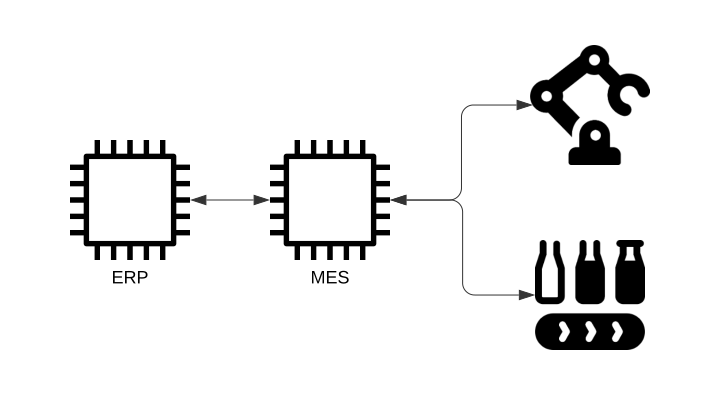
\includegraphics[scale=0.2]{images/Related/ERP.png}
    \caption{Common form of resource planning and management found in Industry 3.0 models. Source: adapted from \cite{Gilchrist2016}.}

    \label{fig:erp}
\end{figure}


The use of \acrfull{cps} allows for greater flexibility in production lines. These new systems are more responsive to factory conditions. In other words, if there is a production issue or a modification needs to be made to a particular product, the production line can respond almost instantly \cite{Gilchrist2016}. For example, if there is a missing part on a conveyor belt or a defective product, the system can quickly alert that there is a problem, and it can automatically or non-automatically take action to mitigate the consequences of that failure. This is one of the reasons why this system is more flexible. With the use of \acrfull{cps}, the \acrfull{erp} system can closely monitor the production line in real-time, giving rise to a new type of software known as \acrfull{serp}.

\begin{figure}[ht!]
    \centering
    \includegraphics[scale=0.2]{images/Related/SERP.png}
    \caption{New form of resource planning and management found in Industry 4.0 models. Source: adapted from \cite{Gilchrist2016}.}

    \label{fig:serp}
\end{figure}

The main challenges encountered in implementing Industry 4.0 are divided into two parts: management of the newly implemented technologies and technical challenges specific to each technology involved. For example, the first challenge is related to the lack of financial resources, skilled people, lack of security or understanding of the technologies. The second challenge concerns the challenges related to connectivity between technologies, e.g. communication interfaces between specific software, connectivity infrastructure, software creation challenge, complexity, etc. These two branches are the main challenges to put in place this new industry \cite{Rikalovic2022}.

\begin{figure}[ht!]
    \centering
    \includegraphics[scale=0.95]{images/Related/chalanges.png}
    \caption{The image portrays the frequency of challenges associated with the implementation of Industry 4.0 by technological areas. For the formation of this image, 47 of the 67 most relevant articles were used on technological problems in the implementation of technologies linked to this new industry model. Source: \cite{Rikalovic2022}.}

    \label{fig:chalanges}
\end{figure}

One of the challenges is the need for improved cybersecurity. The presence of multiple interconnected devices in an internal or external network raises various security concerns, as factory lines can be targets of hacker attacks, compromising the functionality of a production line or the leakage of sensitive data \cite{Gilchrist2016}. One way to mitigate security issues is the use of a Blockchain-based Authentication System (BSeIn), as proposed by the authors \textcite{LIN201842}. Additionally, another challenge is the encryption of communication between \acrfull{cps} in an industrial network. \textcite{Kreiser2018} discuss methods for creating and communicating encryption keys in a controlled environment simulating a manufacturing line. However, the implementation of security measures is limited by the available resources and the specific problem addressed.

Another challenge reported by \cite{PENAS201752} is the difficulty of integrating the virtual and physical environments. \acrfull{cps} typically employ sensors, processing units, and actuators in their operations. In addition to managing each \acrfull{cps} individually, it is necessary to understand how these units communicate with each other in a large-scale environment, enabling them to adapt to unforeseen conditions. Another problem is the lack of compatibility between real and virtual spaces, as simulations are conducted in a discrete environment, which can introduce uncertainty and imprecision \cite{Rikalovic2022}. Furthermore, the synchronization of a digital twin is a challenge for \acrfull{cps} implementation. The virtual model must be synchronized with the physical system to correctly respond to actions from the external environment. The lack of high fidelity and synchronization poses a significant challenge for the intended operation of \acrfull{cps} \cite{Zhang2017}.



Adapting existing systems to the new methodology is a significant challenge. The lack of training and skills among workers acts as a barrier to modernization, as new technologies require employees to undergo a learning curve, especially if they have been performing the same tasks for years. This can result in a substantial investment for companies, particularly small and medium-sized enterprises, and resistance to change.

Moreover, there is a need to integrate older equipment and systems with new technologies. This may involve updating obsolete components or modifying systems to ensure compatibility. Again, this can represent a considerable investment for companies, particularly small and medium-sized enterprises.

The lack of maturity of the technologies involved challenges their deployment and reliability in the industry. The authors \textcite{Rikalovic2022} report that the \acrshort{cps} do not have a widely implemented technology, few available software and communication delay issues. Not to mention that other technologies that \emph{"smart factories"} use such as: \acrfull{vr} and \acrfull{bda} aidna need to develop much more to be reliable in their employability.


In summary, these approaches to IT (Information Technology) in industry present a possible improvement of the manufacturing process. The Industrie 4.0 model is a trend that aims to promote an industrial revolution toward the use of cutting-edge technologies to increase production performance. This approach allows production lines to be more malleable both to produce products with different characteristics and to respond more quickly to unforeseen events that occur during manufacturing. In other words, it is possible for \acrshort{cps} people to make decisions autonomously or not to both unforeseen events and strategic production changes. In addition, this new industrial model brings out smart products that talk to the production line and allow information about its state to be obtained, which can help predict failures or improve customer satisfaction and have a positive impact on the product value chain \cite{economies6030046}.  However, all these technologies involved bring implementation difficulties, either due to issues involving financial resources, knowledge, security, acceptance, adaptation or maturity of the technologies.  



\section{Digital Twin}
\label{sec:digitalTwin}

The concept of Digital Twin (DT) emerged in 2003 \cite{Mihai2022, Barricelli2019} and was initially discussed by \cite{Grieves2017} in their presentation titled "Conceptual Ideal for Product Lifecycle Management" at the University of Michigan. Figure \ref{fig:digitalTwin} was included in this presentation, illustrating the key elements that would later shape the concept of DT. Although initially presented as a product management technique, it already encompassed the fundamental components that define the concept of \acrlong{dt}.

\begin{figure}[ht!]
    \centering
    \includegraphics[width=0.65\linewidth]{images/Related/CAR.pdf}
    \caption{Conceptual ideal for PLM. Dr. Michael Grieves, University of Michigan, Lurie Engineering Center, Dec 3, 2002. Adapted from: \cite{Grieves2017}.}

    \label{fig:digitalTwin}
\end{figure}

An \acrfull{dt} is a computer-based machine or model that mimics, emulates, mirrors the life of a physical entity. It continuously predicts future states and allows simulating and testing new configurations in order to preventively apply \cite{Barricelli2019} preventive maintenance operations. According to \cite{Mihai2022} such a definition corroborates with the one previously created by the authors \cite{Grieves2017}.  Indeed, the main idea behind the concept remains preserved. However, \acrshort{dt} has gained popularity in various industries and other authors have sought to evolve its definition over time, incorporating technologies such as \acrshort{ai}, machine learning, \acrshort{iot} among others. 


Grieves and Vickers  propose that the \acrfull{dt} concept consists of two systems: the physical system that has always existed and a new virtual system that contains all the information about the physical system. The virtual system is used to model and simulate the physical system in virtual space, allowing to better understand the emergent form and behaviors of the system. That is, the virtual part of the system can allow several simulations to be performed in $N$ different virtual spaces $VS_n$, in order to allow one to understand how the system behaves in these different possible environments. This helps reduce the "We didn't expect that" factor \cite{Grieves2017}.

In simple terms, a \acrfull{dt} is a system of systems. Essentially, a \acrshort{dt} is a system that enables the collection of data from different technologies and contextualizes this information in a virtual representation of an object and its interactions with other elements in its surroundings. It is a technology-based system that replicates the elements, processes, dynamics, and firmware of a physical system in a digital counterpart \cite{Mihai2022}. For example, in a case study conducted in an automotive production line in Turkey, it was collected specific data from machines and applied \acrfull{ml} techniques for data analysis \cite{Mendi2022}. This allowed simulations to be performed to identify potential issues before actual production begins, as well as provide insights on how \acrshort{dt} technology could improve efficiency and reduce downtime in that particular factory. Thus, \acrshort{dt} involves the integration of various technologies to create a virtual model that closely represents a real-world object. Figure \ref{fig:digitalTwinTree} illustrates this concept.

\begin{figure}[ht!]
    \centering
    \includegraphics[scale=0.75]{images/Related/DTTree.png}
    \caption{The Digital Twin’s central role in the Industry 4.0 era. Source: \cite{Mihai2022}.}

    \label{fig:digitalTwinTree}
\end{figure}


There are two types of \acrlong{dt}: \acrlong{dtp} and digital \acrlong{dti}. The \acrshort{dtp} describes the prototype of the physical object and contains the sets of information needed to describe and produce a prototypical physical version capable of producing a virtual version.  These information sets include fully annotated 3D Model, Bill of Materials (with material specifications), Process List, Service List, Numerical Simulations, and so on.  The \acrlong{dti} is a concept that describes a physical product that has a virtual twin attached to it for much of its life cycle. Depending on the required use cases, such a Digital Twin may contain, but is not limited to, the following sets of information: A fully annotated 3D model with sizing and geometric tolerance that describes the geometry of the physical instance and its components, a bill of materials that lists the current and all previous components, a process list that lists the operations that were performed in the creation of this physical instance along with the results of any measurements and tests on the instance, a service log that describes past services performed and components replaced, and operational states captured from actual, current, past actual and future predicted sensor data \cite{Grieves2017}. 
  

The \acrshort{dtp} model is an opportunity to identify and eliminate unforeseen and undesirable situations \cite{Grieves2017}. This type of concept allows people involved in the project to use 3D models created in \acrfull{cad} and \acrfull{cam} software, which allow them to virtually visualize and test their ideas in a simulated environment. Moreover, the use of numerical simulations such as \acrfull{fem}, \acrfull{bda} among others is also common in the design process, allowing the analysis of how the product or system will behave in different conditions and under different loads. In this way, designers can predict possible causes of failure of their product such as: failure due to structure stress, aerodynamics problems, electronic circuit design problems, communication errors between the foreseen technologies, list of required materials, etc. With this initial prototyping defined it is possible to foresee a series of failures and errors in project conception, thus avoiding unnecessary expenses with the construction of prototypes or, in the worst case, of the real product, which would not have the required performance. 

  
It is worth pointing out that \acrshort{dt} cannot be summarized simply as a software \acrshort{cad} \cite{Barricelli2019}.  For a system to be considered an \acrshort{dt}, it needs three functional blocks, these are: a physical asset, a virtual counterpart, and a communication system that allows communication between these blocks. Such a communication medium needs to be a bi-directional information flow channel that allows both output and input of data from the real model to the virtual \cite{Mihai2022}. In this way, a 3D model \acrshort{cad}, can be only one of the parts associated with building the \acrlong{dt}. 



The \acrlong{dti} allows you to understand, predict failures, and countless other possibilities about the product. This type of virtual model can have a range of information from the real product that enables the creation of virtual models that replicate physical systems, products, or assets. These are connected to their real-world counterparts via sensors and data communication networks. This enables the analysis of product histories regardless of the physical location of their counterparts. Data collected from various \acrshort{dti} can be correlated and analyzed to predict future states, helping to improve the maintenance and performance of physical systems. The ability to interrogate \acrshort{dti} provides valuable information to monitor, predict, and optimize the operations of physical systems, products, or assets. Thus, in this kind of virtual model one of the topics that is gaining prominence is preventive maintenance \cite{Grieves2017}. However, this is just one of many possibilities that this concept offers. 
  
  
Currently there are some branches of industry where there is a greater emphasis on the development of applications related to \acrshort{dt}, these sectors are: aviation, automotive, health care and predictive maintenance. The advances in these areas are due to both the potential for improvement and the importance of these areas, be it financial or human. For example, the aviation industry has a great interest in the constant monitoring of aircraft to avoid material damage or accidents with damage to human life. For the case of predictive maintenance, it can also be observed that besides the financial importance, recent technological advances allow this branch to become more and more practical. Currently, there are huge advances in developing techniques and algorithms for the prediction of possible failure points. Thus, these areas allow a great deal of practical advancement both in terms of the justification of the importance of solving potential problems and the recent availability of technologies that make this possible.  



The use of \acrshort{dt} in manufacturing can provide an improvement in process efficiency through task automation and in supporting decision making \cite{ROSEN2015567}. \textcite{Qi2018} also report that the use of \acrfull{bd} allows \acrshort{dt} to achieve improved process efficiency and predictions on data collected along the manufacturing line. For example, the use of \acrshort{bda} allows the attempt to predict possible failure points both throughout the life of a product and the occurrence of failures in machinery involved in its manufacture, figure \ref{fig:digitalTwinBigData}. In this way, \acrshort{bda} has great potential for use in predictive maintenance or for adapting the product to certain standards that satisfy the interests of the end user. \textcite{Tao2017} explore the idea of using \acrshort{dt} for the shop floor of a production line through ways of implementing the concept. That is, methods of implementing a virtual counterpart of the production line. This way, possible points of failure can be analyzed and layout or process optimizations applied. In this way, \acrshort{dt} is currently being used more and more in factories to improve processes and products.

In the aeronautical industry, the use of \acrshort{dt} is used more for the predictive area, that is, to detect the appearance of possible failure points and trigger mitigation systems \cite{Barricelli2019}. By means of statistical methods and with numerical approaches involving multi-physics systems it is possible to estimate possible aircraft failures through initial input data \cite{Benjamin2012}. An example is the case in which \textcite{Bielefeldt2015} propose the use of \acrlong{fem} with \acrshort{dt} to obtain possible failure points on a wing of a commercial aircraft. Thus, currently, the use of \acrshort{dt} has an important role in predicting possible unforeseen events or failures that may occur in an aircraft, which can cause enormous damage to property and human life. With the presence of a system that can previously detect possible errors it is possible to mitigate these occurrences or solve them with correction and safety strategies or techniques. 

\begin{figure}[ht!]
    \centering
    \includegraphics[scale=0.75]{images/Related/cps.png}
    \caption{Information of the life cycle of a product through the use of cybernetic physical systems. Source: \cite{Qi2018}.}

    \label{fig:digitalTwinBigData}
\end{figure}

Recently, the area of medical care is another branch that has been achieving great advances in the implementation of new technologies and techniques. \acrlong{dt} is one of the new concepts being implemented in the healthcare area with the goal of creating a virtual system of the human body or its organs in order to achieve the goal of predicting possible diseases or malfunctions of the human body, as well as managing the availability of assets in a hospital. The \textcite{johns_2016} made use of \acrshort{ann} to perform simulations and make the best possible decisions for managing its resources, which is crucial for saving lives. Another case was the use of a \acrshort{dt} by Siemens Healthineers at Mater Private Hospitals (MPH) in Dublin \cite{gilligan_digital_2018}. In this case study, the hospital had a lack of space, beds, delays, and high patient demand. To solve these problems, Siemens Healthineers redesigned the radiology department with the development of a \acrshort{ann} to manage the department and its operations. With this, a \acrshort{dt} of the department was obtained, allowing simulations to be performed to find an optimal layout and control and monitoring of tasks. Another example of \acrfull{dt} is the \emph{The Living Heart} \cite{Levine2022}, Figure \ref{fig:digitalTwinHeart}, this project allows scientists to simulate the human heart. It allows a realistic, multi-phase simulation to be performed, which takes in various physical fields such as electromagnetic, fluid dynamics, and mechanics. In this way, scientists can use this tool to aid studies of how certain physical stresses or cardiovascular diseases may impact the functioning of this organ. 

\begin{figure}[ht!]
    \centering
    \includegraphics[scale=0.65]{images/Related/heart.png}
    \caption{Stresses  simulation depicted on a 3D rendering of the Living Heart Model. Source: \cite{Levine2022}.}

    \label{fig:digitalTwinHeart}
\end{figure}


In summary, the concept of \acrfull{dt} has remained quite stable since its creation in 2002, undergoing adaptations to the technological changes that have been appearing. The \acrshort{dt} is formed by two parts: the physical system and the virtual system. The function of the \acrshort{dt} is to contextualize data from different technologies into a virtual representation of an object and how it interacts with its surroundings. In this way, various technologies can be integrated into this system such as: \acrlong{ann}, \acrlong{bda}, \acrlong{iot}, \acrlong{vr}, \acrlong{vr} among others. With this data generated and processed, it is possible to obtain data about: possible future failures, location information, current physical state, end user interests about the product, etc. In general, \acrshort{dt} is part of the new industrial revolution with enormous potential to reduce costs and increase the productivity of production lines, besides enabling the final product to have a longer life and be safer. 
\section{Review of current traceability systems in the  industry}\label{section: woodFurnitureIndustryTraceabilityReview}

Currently, traceability is employed in several productive sectors, presenting a wide range of applications. Among them are the implementation of \acrfull{mcp} \cite{ZHONG2013}, stock controls \cite{Anssens2011, Yue2011}, production control \cite{Engelhardt2012}, counterfeit prevention \cite{Rida2007}, among other possibilities. The use of a traceability system can significantly improve the execution of tasks in a factory, allowing not only greater control of inventory, but also of the processes themselves. By identifying critical points in production, it is possible to implement actions to mitigate their occurrence and, consequently, make processes more efficient \cite{Chua2012}.


Nonetheless, the comprehension of the traceability concept is indispensable. As per the ISO 9000:2015 standard \cite{iso_9000_2015}, traceability is characterized as the "capacity to trace the history, application, or location of that which is under consideration." To elucidate, within the confines of a production line, traceability denotes the competency to procure an exhaustive historical record pertinent to the product or process. Diverse mediums may be employed for the storage of this information, ranging from paper-based systems to electronic or semi-electronic methodologies.

Subsequently, it is plausible to contemplate the implementation of a hybrid system. Such an approach amalgamates the utilization of conventional paper-based systems with the deployment of digital technologies. This synergy augments the performance metrics associated with tracing products, processes, and the archival of production and inventory records \cite{Qu2012-hw, ZHONG2013, Gilchrist2016}. The architecture of a hybrid system encompasses an assortment of components, including but not limited to printed documents, spreadsheets, manual entries, Enterprise Resource Planning (ERP), and Manufacturing Execution Systems (MES).


However, the hybrid system faces challenges in achieving real-time traceability. One possibility to overcome these obstacles is to incorporate \acrfull{iot} and \acrshort{m2m} communication components, enabling a real-time connection to the \acrshort{erp} or allowing decision making without the intervention of an intermediary agent. The integration of advanced technologies can significantly enhance the efficiency and adaptability of the hybrid system, contributing to greater flexibility and accuracy in the traceability of industrial processes \cite{Gilchrist2016}.

\subsection{Use of RFID for traceability}\label{RFIDtraceability}

The implementation of \acrfull{rfid} sensors is vastly employed in the traceability of components in industry, with applications in various \cite{ZHONG2013, Qu2012-hw, Anssens2011, Engelhardt2012, Rida2007} sectors. The initial concept of RFID dates back to Harry Stockman's paper entitled "Communication by Means of Reflected Power," published in 1948. The idea demonstrated great relevance in aircraft identification by the military sector, especially due to the advances in radar development that occurred during World War II \cite{Landt2005}. This technological innovation allowed for significant improvements in tracking efficiency and accuracy, paving the way for broader industrial and commercial applications in the future.

However, the implementation of RFID technology requires a specific infrastructure, the feasibility of which can vary depending on the added value provided by its use. For the RFID system to function properly, some fundamental components are necessary, such as: an antenna, a transceiver, middle-ware software, a database, and a transponder \cite{MCFARLANE2003365}. Figure \ref{fig:rfid} illustrates the typical configuration of an RFID system.

\begin{figure}[h!]
    \centering
    \includegraphics[width=.65\linewidth]{images/Development/chap3/g1126.png}
        \caption{Simple schematic of an Auto ID system. Source: \cite{MCFARLANE2003365}}

    \label{fig:rfid}
\end{figure}

In this context, the analysis of the feasibility of adopting \acrshort{rfid} technology should consider the costs and benefits associated with its implementation. The necessary infrastructure might represent a significant investment, which should be justified by the expected return in terms of operational efficiency, error reduction, and optimization of the involved processes. Therefore, the decision to adopt \acrshort{rfid} technology should be based on a thorough evaluation of the specific needs of each application and the value it can effectively add.


The selection of technologies to be used in the \acrshort{rfid} system has direct implications on the costs associated with its implementation. There are three categories of \acrshort{rfid} tags available on the market: passive, active, and battery-assisted passive. Each type has distinct characteristics, which influence both the performance and costs of the system. Among the three options, passive tags are the most economical. These tags do not have an internal battery and, consequently, are powered by the energy transmitted by the reader's antenna. Despite being more financially accessible, passive tags have a limited range and can be affected by interference caused by metallic materials and liquids in the environment. On the other hand, active and battery-assisted passive tags, although more costly, offer a greater range and higher resilience to interference \cite{Lee2012}. The choice between these types of tags should take into account the specificity of the application, such as the need for a greater range or tolerance to interference, as well as the availability of financial resources for investment in the \acrshort{rfid} system infrastructure.


The feasibility analysis for the implementation of an inventory management system using \acrshort{rfid} technology is a complex task, as it requires the weighing of multiple factors, such as the predictability of inventory flow, fixed costs, and especially, the technologies involved in the process. Several studies have been conducted to assess the financial feasibility of using \acrshort{rfid} in different contexts.

\textcite{Yue2011}, for example, conducted a simulation of the feasibility of using \acrshort{rfid} in a pharmaceutical supply chain. The authors concluded that, using the \acrfull{npv} method, the venture might not be viable. Therefore, they suggested using the \acrfull{rov} method for a more accurate analysis.

In contrast, \textcite{Ustundag2007} conducted a case study in a parcel delivery company and found that the venture is viable, although the return time varies according to the type of \acrshort{rfid} tag chosen. It is worth noting that this case study does not provide detailed information.

Finally, \textcite{Lee2012} presented an improved methodology for the financial evaluation of investment in radio frequency identification systems. In this paper, the authors introduce a mathematical model capable of quantifying the feasibility of the venture, taking into account inventory flow, fixed costs, and \acrfull{jit} or \acrfull{eoq} inventory models. In this model, the authors address three main aspects:

\begin{enumerate}
  \item Investment in order efficiency;
  \item Investment in JIT efficiency;
  \item Simultaneous investment decisions in \acrfull{rfid}.
\end{enumerate}

The mathematical model proposed by \textcite{Lee2012} is composed of four cost components: ordering cost during a planning period ($\frac{OD}{Q^{*}}$), the efficiency factor of the process tied to \acrshort{rfid} technology (R), inventory holding cost ($ \frac{HQ^*}{2} $), \acrshort{jit} efficiency (I), order efficiency investment cost (K), and \acrshort{jit} efficiency investment cost (V). 

 In this model, the authors address three main aspects, one of which is \acrshort{jit} efficiency, which is defined as the degree to which the time interval between the delivery point and the consumption/production time is reduced by investment V.


However, for the case of the company that is the subject of the current work, the inventory flow is much smaller compared to the three previously analyzed works, in addition to involving products that may not have such a high added value. For this reason, the adoption of the RFID system may not be a plausible approach.

\subsection{Use of QR Code for traceability}\label{QRtraceability}

The QR code, conceived by Toyota subsidiary Denso Wave in 1994, was established with the purpose of facilitating the tracking of automotive components. The motivation behind the development of the QR code resided in the limitation of the information capacity of traditional bar-codes, which can only accommodate 20 alphanumeric characters. This technological innovation proved its efficiency by providing greater control and accuracy in tracking the parts used in the automotive industry \cite{Tiwari2016}.

Over time, the application of the QR code expanded to various other sectors, establishing itself as a valuable tool for enhancing traceability, inventory management, commercial applications, event ticketing, electronic transactions, and other relevant functionalities \cite{Tiwari2016}.

The operation of the QR code system is based on two main components that work together to encode and decode information: the QR code encoder and the decoder. The encoder is responsible for processing the data and generating the QR Code, while the decoder extracts and interprets the data stored in the QR code, see figure \ref{fig:qr}. The structure of the QR Code is formed by modules, which are the black and white dots that make up the code. These modules are organized into symbols ranging from Version 1 to Version 40, each with a distinct configuration of modules, starting with Version 1, which contains 21 × 21 modules, up to Version 40, with 177 × 177 modules \cite{iso_18004_2015}. This organization allows for the efficient encoding and decoding of information, ensuring the effectiveness of the QR Code as a tool for traceability and data storage in various contexts and applications \cite{Tiwari2016}.


\begin{figure}[h!]
\centering
\includegraphics[width=.65\linewidth]{images/Development/chap3/QR.pdf}
\caption{Working (overview) of QR Code. Adapted from: \cite{Tiwari2016}}
\label{fig:qr}
\end{figure}

Despite the numerous advantages of QR Code over barcode, especially in terms of speed and data storage capacity, the QR Code still has capacity limitations. Each version of the QR symbol has a maximum data capacity, which depends on the amount of data, the type of character, and the error correction level \cite{Tiwari2016}. In other words, as the amount of data increases, more modules are needed to compose the QR Code, resulting in a larger QR Code symbol, see table \ref{tab:qrcode-capacity}. Therefore, although the QR Code offers significant benefits in terms of traceability and information storage, it is important to consider its capacity limitations when selecting the best solution for a given context or application.

\begin{table}[!ht]
\begin{tabular}{llllllll}
\hline
\multicolumn{8}{c}{DATA CAPACITY OF QR CODE VERSION 40 } \\
\cline{1-8}

Version             & Modules                  & ECC Level & Data Bits & Numeric & Alphanumeric & Binary & Kanji \\
\cline{1-8}


\multirow{4}{*}{40} & \multirow{4}{*}{177x177} & L         & 23,648    & 7,089   & 4,296        & 2,953 & 1,817 \\
                    &                          & M         & 18,672    & 5,596   & 3,391        & 2,331 & 1,435 \\
                    &                          & Q         & 13,328    & 3,993   & 2,42         & 1,663 & 1,024 \\
                    &                          & H         & 10,208    & 3,057   & 1,852        & 1,273 & 784 \\
\cline{1-8}
\end{tabular}
\caption{QR Code Capacity. Adapted from: \cite{Tiwari2016}}
\label{tab:qrcode-capacity}
\end{table}

In conclusion, the QR code, initially designed to optimize the tracking of automotive components, has experienced a remarkable evolution since its creation, establishing itself as a multi-functional and comprehensive tool, applicable in various sectors. The ability to store information efficiently, coupled with the ease of use through mobile devices and comparatively lower cost compared to other solutions such as Radio Frequency Identification (RFID), gives the QR code a valuable solution in improving traceability and data management in various contexts. However, it is crucial to consider the inherent limitations of the QR code's capacity when selecting the most suitable alternative to meet specific demands for tracking and information storage. In this sense, the QR code persists as a technological innovation of relevance, capable of providing significant contributions to the efficiency and effectiveness of traceability processes, as well as to the storage and sharing of information in different environments, within its limitations.

\section{State of the Art in Traceability for Wood Work}\label{section:stateOfArt}
One of the driving forces behind the development of this work is the noticeable scarcity of research and solutions addressing the traceability of the wood fabrication process. In the academic circle, a limited number of existing solutions are being explored and studied. Indeed, only a handful of scientific articles that delve into this topic were identified. The majority of the available literature predominantly concentrates on supply chain aspects and employs technologies such as Radio Frequency Identification (RFID),  block-chain, QR Code, Fingerprint Methods, that can be utilized to address the identification of timber logs.

The employment of Radio Frequency Identification (RFID) technology offers substantial advantages for real-time tracking in the wood supply chain. However, its feasibility hinges on an in-depth financial analysis concerning the impact of implementation \cite{Ustundag2007}. \textcite{Lee2012} present a methodological and comprehensive analysis in their article, which considers the substantial initial investments required for the deployment of this technology. In conclusion, the feasibility of adopting RFID technology will depend on the scale of application and the specific aspects that the technology aims to address, as well as the inventory model that will be employed, whether it be \acrfull{jit} or \acrfull{eoq}.

In their study, \textcite{hultgren2018blockchain} present an approach employing block-chain technology for the traceability of the supply chain in the timber production process. Furthermore, their approach facilitates the integration of additional stages into this block-chain model. However, it's important to note that the model does not support real-time monitoring of the traceability. To achieve real-time tracking, the incorporation of supplementary technologies would be necessary. Block-chain, in this context, offers transparency and security, but for more dynamic tracking, complementary tools and technologies need to be considered.

In another case study conducted by  \textcite{Amaya2022}, a system based on a web solution coupled with QR Codes was utilized for the tracking of timber logs. The system developed by the authors essentially allows IoT devices or users to input data into the system which can then be accessed and monitored through a web platform. Moreover, in order to facilitate easy tracing of timber logs in the cutting and extraction environment, QR Codes are attached to the logs. When scanned, these QR Codes redirect the user to the web application, providing a historical record of information pertaining to that specific log. This approach combines the accessibility of web platforms with the ease of QR Code technology, creating an efficient and user-friendly tracking system for timber management.

In a scholarly article authored by  \textcite{Schraml2020}, an attempt is made to establish a fingerprinting standard for timber logs. The authors have developed a methodology which employs spectral scanning systems to acquire detailed hyperspectral data (HSD) of timber. Subsequently, high-resolution images are captured and processed through computer vision techniques for the segmentation of individual timber pieces. Through this approach, the authors manage to extract detailed information about each timber log, effectively characterizing each log with unique features. In a parallel development, \textcite{Sun2021} also utilize a computer vision-based approach for deriving fingerprints of timber logs, but through a pure \acrfull{cnn} approach. In their methodology, the authors employ the AKAZE computer vision technique to identify wood grain patterns for each timber log, which can then be used to uniquely identify them. Both these studies highlight the innovative use of computer vision and spectral analysis techniques in establishing unique identifiers for timber logs, which can have significant implications for traceability and management in the wood work industry.

% \subsection{Use of Artifical Inteligency in traceability}\label{ArtificialIntelligencetraceability}

% The use of barcodes and RFID is a widely adopted practice in product tracking, both in production and in stock. However, these methods present some limitations. The use of barcodes, for instance, has a restricted capacity for information storage and can be easily damaged, which hampers reading. Additionally, the employment of RFID also faces the issue of potential damages, besides the high costs associated with the infrastructure required for its operation \cite{Pihir2011}.  \textcite{Elisabeth2011} also mention the difficulties of using RFID for certain types of materials that can interfere with the reading of radio waves, which may demand more robust tags and further increase the involved costs.

% Over the past few years, the exponential growth of e-commerce has driven significant advancements in goods warehousing management, due to the increase in the scale and complexity of operations involved in this scope. Currently, companies are employing a broad range of advanced technologies, such as QR codes, machine vision systems, communication modules, microcomputers, servers, and RFID, which allow the integration of sophisticated systems that apply artificial intelligence in strategic decision-making. This technological evolution has proven to be crucial in improving storage management and optimizing the efficiency and effectiveness of operations, meeting the growing demands and challenges imposed by the constantly expanding e-commerce \cite{Hristov2022}.

% The application of artificial intelligence in traceability processes transcends decision-making in the industrial context. For example, \textcite{Hristov2022} employed \acrfull{cnn} in object detection, enabling robots to identify items in a storage center and, consequently, speeding up decision-making in performing their tasks. This innovative approach demonstrates the potential of artificial intelligence to enhance the efficiency and precision of traceability processes, as well as allowing for inventory traceability, contributing to greater adaptability and dynamism in the operations of storage and movement of goods.

% In contrast to traditional item tracking methods,  \textcite{Patel2020} propose an innovative approach using \acrshort{cnn}, specifically with the ResNet-50 architecture. In this methodology, they employed transfer learning techniques to enable agile adaptation of the data model in scenarios with a limited amount of training images. Consequently, they achieved an image tracking rate of 4 \acrfull{fps}, considering the adopted software and hardware settings, enabling real-time object traceability.

% Another important aspect to be considered is the possibility of customizing \acrshort{cnn}s to meet the specific needs of different industries and sectors. Through the use of appropriate architectures and algorithms, it is possible to develop tracking solutions adapted to the particularities of each scenario, optimizing the efficiency and effectiveness of operations.



\cleardoublepage
\chapter{Material and Methods}\label{cap:studyOfTools}

This chapter endeavors to elucidate the technological tools and methodologies deployed across various stages of this project’s development. Specifically, in Section \ref{section:imageProcessing}, an introduction to certain image processing methodologies, notably Gaussian filtering and Canny edge detection, is presented. Both these image processing techniques form the crux of algorithms employed for acquiring distinct edges of wood pieces. This, in turn, facilitates the automatic classification of the geometries of the wood leftovers.

In Section \ref{section: System}, the devices employed in the traceability solution proposed for wood leftovers are delineated. Furthermore, in Section \ref{section:comunication}, the communication methodologies between the various services and devices that constitute the solution are explicated. Such information is vital for the definition of the system's architecture.
 
 
In Section \ref{section:conceptulaDataModel}, a conceptual data model is developed, which is integral for an in-depth analysis of the company's operations and for crafting an architecture tailored to its specific requirements. Additionally, aspects related to the databases employed are elucidated in Section \ref{section:mmDataBase}, furnishing insights regarding the tools that were selected for the construction of the system's overall architecture.

Moving on to Section \ref{section:security}, crucial aspects regarding security that were employed in the overall system architecture are delineated.

The tools employed for file sharing are defined in Section \ref{section:fileSharing}, and Section \ref{section:fileSharing-webserver} details the necessary aspects and the servers used for potential project monitoring.

Section \ref{section:ProjectTraceability} addresses the methodological aspects involved in project traceability, and finally, Section \ref{section:LeftoverTraceability} describes the methods employed for leftover traceability.

\section{Digital Image Processing}\label{section:imageProcessing}

Digital image processing is a field that addresses the manipulation, analysis, and interpretation of digital images, which are discrete two-dimensional functions, $f(x_i, y_i)$, composed of elements called pixels. This discipline encompasses a wide spectrum of applications and is related to areas such as image analysis and computer vision. Digital image processing can be divided into low, medium, and high-level processes. Low-level processes involve pre-processing and image enhancement, while medium-level processes deal with segmentation, description, and classification of objects. On the other hand, high-level processes seek to make sense of sets of recognized objects and perform cognitive functions associated with vision. Digital image processing encompasses processes that work with image inputs and outputs and also processes that extract attributes from images, including the recognition of individual objects, successfully applied in various areas of social and economic value \cite{gonzalez_rafael_c_digital_2018}.

In this multidisciplinary field, a wide range of techniques and algorithms is employed to optimize image quality, enhance features of interest, and facilitate the extraction of valuable information. Such approaches can be applied in various contexts, ranging from improving the quality of images obtained by digital photographic devices to the analysis of data in images for specific applications \cite{ekstrom2012}.

However, as reported by \textcite{mcandrew2004introduction}, image processing addresses two distinct and fundamental aspects:
\begin{enumerate}
\item Enhance the pictorial information for human interpretation.
\item Make the image more suitable for autonomous machine perception.
\end{enumerate}

The first aspect refers to enhancing the pictorial information of an image for human interpretation, which involves improving the visual appearance of the image. The second aspect aims to make the image more suitable for autonomous machine perception, which implies simplifying and organizing the image efficiently. These two conditions require distinct and specialized procedures, and a procedure that satisfies one condition may not necessarily satisfy the other. As can be seen in figure \ref{fig:imageProcessingExample}, despite the processed image presenting greater significance for a contour analysis, it may not have an attractive aspect to the human eye \cite{mcandrew2004introduction}.



Additionally, image processing plays a crucial role in the development of computer vision systems and machine learning, allowing electronic devices and machines to interpret and understand visual information in a manner analogous to human perception. This ability to process and analyze images is essential for devising innovative solutions in areas such as robotics, industrial automation, security and surveillance, facial recognition, among others.

In summary, image processing constitutes a comprehensive and multidisciplinary field of study, encompassing knowledge from computer science and engineering, aiming to improve the quality of digital images and extract relevant information for a wide range of applications. Through the application of advanced techniques and specialized algorithms, image processing significantly contributes to the progress of computer vision and machine learning, driving innovation and technological development in various sectors.


\subsection{Gaussian Filtering}

One of the critical steps developed in this project is the ability to observe the geometry of a part, and in order to achieve this, it is necessary to apply the Gaussian filter, which will be explained in the following section.

Applying a filter to an image implies performing a convolution operation. In the continuous context and with a single variable in the domain, this operation can be represented by the equation \ref{eq:convolution} \cite{spiegel_schaums_1974}. However, when working with digital images, it is common to employ an adaptation of this equation for discrete media in a two-dimensional domain, which makes use of a base matrix, called a kernel, as illustrated in the equation \ref{eq:convolution-discreet} \cite{gonzalez_rafael_c_digital_2018}. The kernel is used to assign weights to neighboring points of a specific point in the image, modifying their values and resulting in an image with altered pixels. During convolution, the kernel is applied to each point in the image, multiplying its weights by the values of adjacent pixels, see image \ref{fig:kernel-convolution}.

\begin{equation}
(f * g)(t) = \int_{-\infty}^{\infty} f(\tau) \cdot g(t-\tau) d\tau
\label{eq:convolution}
\end{equation}

\begin{equation}
(f * w)(x_i, y_i) = \sum_{s=-a}^{a} \sum_{t=-b}^{b} f(x_i +s, y_i +t) \cdot w(s, t) \quad \forall i \in \mathbb{N}
\label{eq:convolution-discreet}
\end{equation}\\


\begin{figure}[ht!]
\centering
\includegraphics[width=.65\linewidth]{images/Development/chap3/kernel.png}
\caption{Kernel convolution representation on a digital image. Source: \cite{gonzalez_rafael_c_digital_2018}.}
\label{fig:kernel-convolution}
\end{figure}



The linear spatial filters are widely used and employ a kernel that performs the sum of products between the original image and the kernel itself, as shown in Figure \ref{fig:kernel-transformation}. The size of the kernel defines the neighborhood of operation, while its coefficients determine the nature of the filter. It is worth noting that different kernels can be applied for different purposes, such as enhancing sharpness, highlighting details, or detecting edges \cite{gonzalez_rafael_c_digital_2018}.



Moreover, various types of filters can be combined to achieve more sophisticated results. For example, smoothing and enhancement filters can be used together to produce sharper and more detailed images \cite{mcandrew2004introduction}. The process of applying filters can be repeated several times until the desired result is obtained; however, it is essential to consider that excessive use of filters can result in information loss and the presence of artifacts in the final image.

Filters are characterized by the dimension of the kernel and their associated weights, establishing the nature and behavior of the filter. The kernel dimension has a considerable impact on the final result of the filtering, defining the number of adjacent pixels considered during the convolution operation. Larger kernels promote a more pronounced smoothing effect and noise reduction, although they can lead to loss of fine details, while smaller kernels enable a more pronounced selective effect and preservation of fine details, but with greater sensitivity to noise presence. The distribution of kernel weights is another crucial factor that influences the filter's performance. An example is the case where a bell curve is used, as shown in Figure \ref{fig:gaussian3d}, to establish the relationship of weights $w(s, t)$. The Gaussian distribution is commonly used for this purpose, which is an exponential function that reaches its maximum at the central point of the kernel and rapidly decreases towards the edges, as shown in Equation \ref{eq:gaussian-distribuition}. This means that pixels closer to the center of the kernel will have more weight than pixels farther away, resulting in more efficient smoothing without losing fine details. Therefore, the choice of kernel and weight distribution is crucial to obtain appropriate results in image processing \cite{gonzalez_rafael_c_digital_2018, mcandrew2004introduction, DHAEYER1989}.

\begin{equation}
    w(s,t) = G(s, t) = K e^{-\frac{s^2 + t^2}{\sigma^2}} \quad  :\ K \in \mathbb{R}
    \label{eq:gaussian-distribuition}
\end{equation}

\begin{figure}[h!]
\centering
\includegraphics[width=.65\linewidth]{images/Development/chap3/gaussian_3d_plot.pdf}
\caption{Gaussian distribution.}
\label{fig:gaussian3d}
\end{figure}


The appropriate selection of the Gaussian kernel dimension is an essential aspect in image processing. Often, a kernel size that does not exceed $6\sigma$ is adopted, as values beyond $3\sigma$ from the center become practically irrelevant to the final result. This phenomenon arises from the fact that the Gaussian function has significantly reduced values at a distance greater than $3\sigma$ from its center, making them less important for filtering. Opting for a kernel of suitable dimensions is crucial to ensure an optimal balance between computational efficiency and the quality of the filtering process \cite{gonzalez_rafael_c_digital_2018}.



\subsection{Canny Edge Detection}\label{subsection:Canny-edge-detection}

Just as the Gaussian filter is used to remove noise from the image, the Canny filter is employed to detect edges. This process is essential for obtaining the geometries of the leftover materials and thereby automating the measurement process of a remnant. The fallowing section will explain this process. 

The study of vertex detection is not a recent research area in science. In the 1960s, researchers \textcite{hubel1968receptive} \cite{hubel1962} conducted pioneering studies to understand the process of vertex detection at the biological level, conducting experiments with monkeys and cats. Later, in the 1970s, researchers \textcite{daniel1971} attempted to mathematically model the perception of vertices by the cerebral cortex, using Fourier Series for this purpose.

However, it was with the popularization of digital images in the 1980s that vertex detection gained more prominence and practical applicability. It was in this context that \textcite{marr1980theory} developed a mathematical analysis for image processing, with the aim of identifying vertices. In this study, the authors used the Laplacian applied to the Gaussian distribution. The contribution of these authors provided a solid foundation for subsequent studies in this area.

Subsequently, \textcite{canny1986} made significant advances in the vertex detection process, optimizing the initial process developed for vertex processing. As a result of their work, a widely known and used filter emerged, which was named the "Canny Filter". This filter became a reference in the field of image processing, offering an effective and robust approach for the precise detection of vertices in various applications \cite{ding_canny_2001}.

Vertices are a characteristic present in images, representing regions where two groups of pixels with similar tones differ. In other words, they are areas where there are abrupt changes in pixel intensity. In real-world images, edges often exhibit blur and display a smooth transition, resulting in thicker edge positions due to the blurring effect. However, from a mathematical point of view, the derivative of a smooth transition is a step function, and the first-order derivative is zero in regions with constant intensity levels and has nonzero values throughout the transition region \cite{Chaple2015}. Therefore, the magnitude of the first-order derivative can be used to detect edges \cite{gonzalez_rafael_c_digital_2018}. Figure \ref{fig: imageBoundary} visually reveals these discussed characteristics.

\begin{figure}[ht!]
\centering
\includegraphics[width=.65\linewidth]{images/Development/chap3/chart.pdf}
\caption{Graphical depiction of a vertex region wherein the digital image $I(s, t)$ exhibits a variation in the intensity of its pixels. Adapted from: \cite{marr1980theory}.}
\label{fig: imageBoundary}
\end{figure}


Thus, as an image represents a function with a domain in two-dimensional space \cite{marr1980theory}, we can calculate its variation using the differential operator nabla \cite{Zhang2020}. The nabla operator applied to the function \(f(x, y)\) is represented by the following equation:


\begin{equation}
    \nabla f(x, y) = \frac{\partial f}{\partial x} \mathbf{i} + \frac{\partial f}{\partial y} \mathbf{j}
\end{equation}

In the context of digital images, it is necessary to adapt this operator. One of the approaches used is the Prewitt-Sobel operator.

The Prewitt operator was initially proposed as a type of edge detection that uses a first-order differential operator. It calculates the intensity difference between neighboring pixels in the vertical and horizontal directions. At edges, this mathematical object is capable of detecting extremes, removing false edges, and smoothing noise \cite{Zhang2020, prewitt1970object}. It can be obtained in the form of equations \eqref{eq:py} and \eqref{eq:px}. These equations represent the kernels of the Prewitt operator that are used to convolve a digital image.

\begin{equation}
    P_t= \
\begin{bmatrix}
-1 & 0 & 1 \\
-1 & 0 & 1 \\
-1 & 0 & 1 \\
\end{bmatrix} 
* I(s, t)
\label{eq:py}
\end{equation}
\begin{equation}
    P_s = 
\begin{bmatrix}
-1 & -1 & -1 \\
0 & 0 & 0 \\
1 & 1 & 1 \\
\end{bmatrix}
 * I(s, t)
\label{eq:px}
\end{equation}

Subsequently, the Sobel operator was developed as an improvement over the Prewitt operator. It introduces a weight of 2 on the central coefficient of the mask, as shown in equations \eqref{eq:gs} and \eqref{eq:gt}. This allows for better noise suppression compared to the Prewitt operator \cite{Zhang2020}. Thus, the Prewitt-Sobel operator is an evolution of the Prewitt operator, incorporating the enhancements introduced by the Sobel operator. The Prewitt-Sobel operator is defined as follows:

\begin{equation}
G_s = \begin{bmatrix}
-1 & 0 & 1 \\
-2 & 0 & 2 \\
-1 & 0 & 1
\end{bmatrix} * I(s, t)
\label{eq:gs}
\end{equation}

\begin{equation}
G_t= \begin{bmatrix}
-1 & -2 & -1 \\
0 & 0 & 0 \\
1 & 2 & 1
\end{bmatrix} * I(s, t)
\label{eq:gt}
\end{equation}
Where \(G_s\) and \(G_t\) are the convolution responses with the Sobel masks in the horizontal and vertical directions, respectively. The process of applying these masks can be observed in Figure \ref{fig: sobelApplyed}.
\begin{figure}[ht!]
\centering
\includegraphics[width=.65\linewidth]{images/Development/chap3/mask.png}
\caption{The image depicts the application of the Sobel operator to an image, which is a commonly used technique for edge detection. Source: \cite{Matthew2020}.}
\label{fig: sobelApplyed}
\end{figure}

Thus, the intensity and direction of the gradient can be obtained through Equations \eqref{eq:arctG} and \eqref{eq:mapprox} \cite{gonzalez_rafael_c_digital_2018, Zhang2020}.

\begin{equation}
    \theta = \arctan \left( \frac{{G_t}}{{G_s}} \right)
    \label{eq:arctG}
\end{equation}

\begin{equation}
    \text{{M}} = \sqrt{{G_s^2 + G_t^2}}
\end{equation}
Which can be approximated in the equation \ref{eq:mapprox} \cite{gonzalez_rafael_c_digital_2018}: 
\begin{equation}
    \text{{M}} \approx \|G_s\| + \|G_t\| 
    \label{eq:mapprox}
\end{equation}

After calculating the gradients, considering their respective directions and magnitudes, non-maximum suppression is implemented. This technique aims to identify and preserve those local maximum points that typically align with the edges of an image. The methodology for this process, although intricate, can be described in an accessible manner. The first step is to determine the direction in which the maximum gradient variation occurs in a specific region. Next, the point of maximum intensity along this direction is identified. Among the various possible points, only this point of maximum intensity is retained, resulting in the elimination of other points that do not correspond to local maxima. Figure \ref{fig: suppression} can be used to illustrate this situation. Let's consider point A located on the edge (vertical direction) of the image. The gradient direction, in this case, is normal to the edge. Points B and C, on the other hand, lie in the gradient directions. Thus, point A is compared to points B and C to determine if it constitutes a local maximum. If this condition is satisfied, point A is considered for the subsequent step. Otherwise, it is suppressed (assigned a value of zero) \cite{canny_opencv_nodate}.

\begin{figure}[ht!]
\centering
\includegraphics[width=.65\linewidth]{images/Development/chap3/opencv.pdf}
\caption{Suppression of non-maximums. Adapted from: \cite{canny_opencv_nodate}}
\label{fig: suppression}
\end{figure}
As a final step, the edge detection process aims to identify truly significant edges, distinguishing them from those that are considered less relevant or false. To achieve this, two threshold values, minVal and maxVal, are established, as shown in Figure \ref{fig: hysteresis}. Edges that exhibit intensity gradients exceeding the maxVal threshold are recognized as true edges, while those with gradients below the minVal threshold are discarded. Edges with gradients whose intensity lies between these two thresholds are categorized as either true or false, taking into account their connectivity. If they are associated with "safe edge" pixels, they are interpreted as legitimate; otherwise, they are eliminated. The appropriate choice of values for minVal and maxVal is crucial to ensure accurate results. This phase is also responsible for removing low-magnitude isolated noise, operating under the assumption that true edges consist of long and continuous lines \cite{canny_opencv_nodate}.

\begin{figure}[ht!]
\centering
\includegraphics[width=.65\linewidth]{images/Development/chap3/hysteresis.jpg}
\caption{Hysteresis Thresholding. Source: \cite{canny_opencv_nodate}}
\label{fig: hysteresis}
\end{figure}

As an example, edge A, whose gradient intensity exceeds the maxVal threshold, is classified as safe. Edge C, even though it falls below the maxVal threshold, is connected to edge A and is thus recognized as a valid edge. However, edge B, despite having intensity above the minVal threshold and being located in the same region as edge C, is not connected to any safe edge. Therefore, it is discarded.

In conclusion, it is emphasized that the Canny filtering method is a robust and efficient approach for obtaining edges in images, based on mathematically optimized models for this purpose. This procedure is structured into several stages that converge to the final result. Initially, noise is reduced by applying a Gaussian filter, followed by the calculation of the intensity gradient, which allows for determining the direction and magnitude at each pixel. Next, the non-maximum suppression phase aims to eliminate pixels that are not at the peak of the gradient, contributing to the accuracy of the method. Subsequently, thresholds (minVal and maxVal) are defined to distinguish genuine edges, ensuring the effectiveness of the technique. Finally, the implementation of hysteresis edge tracking determines that edges with gradient intensity within the threshold range are considered true only if connected to "safe edge" pixels. Thus, the Canny algorithm emerges as a comprehensive and reliable strategy for edge detection and discrimination in digital images, providing high precision and performance to the process.

\section{ Systems}\label{section: System}

 Systems, characterized as systems built around microprocessors and designed to control a specific function or a range of functions, have played a crucial role in various technological applications. Incorporating hardware and software components, they are not intended to be programmed for direct end-user consumption, unlike personal computers, as their programming is focused on executing a specific task, although it allows for different options and choices \cite{heath2002embedded}.

This type of system exhibits an innate ability to interact with the physical world, processing and responding to signals, whether they are analog or digital, thus becoming the cornerstone of numerous contemporary innovations. The functional core of these systems is anchored in the Central Processing Unit (CPU), which coordinates all system activities. Simultaneously, a micro-controller, by integrating various peripheral components into a single circuit, contributes to the efficiency and economy of these systems \cite{peckol2019embedded}.

The importance of  systems is unequivocally evident in their extensive range of applications, spanning from common household appliances to the sophisticated Internet of Things (IoT). This breadth of use illustrates their crucial and indispensable role in contemporary technological infrastructure. In the context of this work, one of the employed  systems was the Jetson Nano\textsuperscript{\textregistered}, as seen in Figure \ref{fig:jetson}. This system, specifically designed for image processing, stands out particularly when applied in image recognition using \acrfull{cnn}, confirming its specialization and effectiveness in this domain \cite{nvidia_jetson_2019}.

\begin{figure}[ht!]
\centering
\includegraphics[width=.65\linewidth]{images/Development/chap3/JetsonNano.png}
\caption{Graphical representation of Jetson Nano\textsuperscript{\textregistered}. Source: \cite{nvidia_jetson_2019}}
\label{fig: jetson}
\end{figure}

Another hardware used was the U3-36L0XC-C\textsuperscript{\textregistered} camera, manufactured by IDS\textsuperscript{\textregistered}. This camera is capable of automatically producing high-quality images and videos, efficiently adapting to variations in object distance and unfavorable lighting conditions. It is equipped with the CMOS AR1335\textsuperscript{\textregistered} sensor, manufactured by Onsemi\textsuperscript{\textregistered}, which has a resolution of 13.10 megapixels. This sensor, operating based on rolling shutter technology, has a resolution of 4200 x 3120 pixels and a pixel size of 1.1µm, offering a frame rate of 20.0 fps, ensuring the capture of detailed and accurate images of the captured object \cite{ids_imaging_development_systemsu3-36l0xc_2023}.


\begin{figure}[ht!]
\centering
\includegraphics[width=.65\linewidth]{images/Development/chap3/IDS_CAMERA.png}
\caption{Graphical representation of Jetson Nano\textsuperscript{\textregistered}. Source: \cite{nvidia_jetson_2019}}
\label{fig: jetson}
\end{figure}

In this work, the adopted methodology for the data flow begins with the image capture process by the U3-36L0XC-C\textsuperscript{\textregistered} camera. Subsequently, these images are transmitted to the Jetson Nano\textsuperscript{\textregistered} hardware via a wired connection, ensuring the quality and integrity of the transferred data.

In the next stage, these images undergo treatment and processing on the Jetson Nano\textsuperscript{\textregistered}. After completing this crucial step, the processed data is transferred via the HTTP protocol to the server located at Mofreitas.

Finally, with the data stored on the server, it becomes possible to make it available for access and manipulation through a Restful \acrfull{api}\footnote{An Application Programming Interface (API) provides an abstraction for a problem and specifies how clients should interact with software components that implement a solution to that problem. APIs define reusable building blocks that allow incorporating modular functionality into end applications \cite{reddy2011api}}. This enables the integration of this data into the web platform, allowing it to be used for multiple purposes. Thus, the present methodology outlines an effective balance between data transmission security and efficient integration among the various elements of the system. A broader view of the data flow can be seen in Figure \ref{fig:simpleModelOfTheDataProcess}.

\begin{figure}[h!]
    \centering
    \includegraphics[width=.65\linewidth]{images/Development/chap3/LeftOver.pdf}
    \caption{Simplified Model of Communication between  Systems and the WW4 Server.}
    \label{fig:simpleModelOfTheDataProcess}
\end{figure}

\section{Communication Between Devices}\label{section:comunication}

Establishing robust methodologies for communication between devices is an essential component in this project, which, in turn, requires a deep understanding of the technologies integrated in this stage.

At the core of this project is the Orion-LD GE, a software specialized in managing data from various devices, which provides a standardized communication interface between these devices, the NGSI-LD API. This interface, based on the REST model\footnote{A REST (Representational State Transfer) API is a set of conventions for building and interacting with web services. It uses HTTP methods to manipulate data and is generally used to allow communication between different systems in an efficient and standardized way. A REST API is stateless, that is, each request from the client to the server must contain all the information necessary to understand and fulfill the request, without the server having to remember previous requests \cite{Mark2011}.}, It uses the HTTP protocol for communication, making it efficient and practical. However, a peculiarity of this interface is that it only supports data that can be serialized in JSON format, thus standardizing and unifying communication between devices. However, this characteristic imposes some limitations, such as the inability to transmit binary data. Therefore, it is established that the adopted communication method must not only follow the Restful model but also be able to serialize data in JSON format in order to maximize the effectiveness of the interaction between devices \cite{etsi2023}.

However, it is important to note that the U3-36L0XC-C camera and the Jetson Nano, mentioned earlier in Section \ref{section: System}, adopt a different communication approach. Specifically, the U3-36L0XC-C camera communicates with the Jetson Nano through serialized ports, ensuring a constant flow of data \cite{ids_imaging_development_systemsu3-36l0xc_2023}. On the other hand, the Jetson Nano has the ability to establish direct communication with the server using the MQTT protocol\footnote{MQTT (Message Queuing Telemetry Transport) is an open and efficient messaging protocol designed for bandwidth-constrained environments such as Machine-to-Machine (M2M) and Internet of Things (IoT) where a compact code representation is required \cite{banks2019mqtt}.}. The latter proves particularly useful in Internet of Things contexts, where energy efficiency and bandwidth optimization are vital considerations.


Another technology employed in this project is the \acrfull{wsgi} application, which essentially serves as the backend service built in Python. This application interacts primarily with three entities: the  system Jetson, the Orion-LD Context Broker, and the Email server. To communicate with the first two entities, Jetson and Orion-LD, the HTTP protocol is used. For communication with the Email server, a different network protocol is employed. The \acrfull{smtp} protocol allows the \acrfull{wsgi} application to establish direct and reliable communication with the Email server, which is especially useful for sending transactional emails. These emails may include registration confirmations, password change notifications, and other relevant communications for users. Thus, each entity has a specific communication method, contributing to the overall efficiency of the project.


\section{Conceptual Data Model}\label{section:conceptulaDataModel}

The design of a data model constitutes a fundamental step in this project. However, for proper execution, it is essential to formulate a methodology. In this perspective, the definition of a series of structured procedures becomes necessary to guide and provide a framework for its implementation. Thus, in this section, we propose to elucidate the methodology for this procedure while highlighting the tools that have been strategically employed during the process.

The digitization of the business world relies on one crucial step: the transfer of real-world ideas into the digital realm. In other words, the creation of a Conceptual Data Model (\acrshort{cdm}). This phase encompasses the abstraction and representation of data relevant to an organization's reality, transforming the real world into a processable and understandable form for the digital system. When executed rigorously and appropriately, the \acrshort{cdm} has the potential to significantly enhance system functionality and efficiency. Moreover, it contributes to error minimization, provides better alignment with user needs, and offers the ability to effectively adapt to changing user demands. Last but not least, a well-implemented \acrshort{cdm} can reduce the inherent costs of system development and maintenance \cite{Batra1995}.

Therefore, the starting point for creating a data model is to acquire a comprehensive understanding of the processes. To illustrate, Figure \ref{fig:MofreitasWorkflow} provides an amplified visualization of the workflow. Simplifying, it all starts with a project design request from the client. As the specifications are detailed by the client, the design department strives to create drafts until the desired outcome is achieved by the client.

\begin{figure}[H]
    \centering
    \includegraphics[width=.98\linewidth]{images/Development/chap3/Mofreitas Process.pdf}
    \caption{An abstraction of the process flow that unfolds during the execution of a project at Mofreitas.}
    \label{fig:MofreitasWorkflow}
\end{figure}

Subsequently, the design department comes into play to verify the availability of resources in the factory and proceeds to create the necessary files for the production of wooden furniture. This documentation includes cutting lists, files for \acrfull{cam}, 3D images, and files for \acrfull{cad}. Once this stage is completed, the project is forwarded to the factory, initiating the manufacturing phase. This stage involves a myriad of machines and procedures, whose combination may be unique to each project.


Once all the pieces are manufactured, the furniture is sent to the assembly line. At this stage, a pre-assembly takes place to identify possible manufacturing errors or any missing components. Once the integrity of the product is confirmed, it proceeds to the packaging phase, which is carried out with the aim of optimizing space during transportation.

Finally, after the dispatch of the pieces, the culmination of the process is the reassembly of the project at the client's location, marking the completion of the service provided by Mofreitas.

In the context of the technologies applied in this project, as mentioned in Section \ref{section:comunication}, we can identify the concrete application of certain key concepts. The Fiware\textsuperscript{\textregistered} platform, for example, utilizes context entities, which represent both physical objects and logical concepts, to build a data model that serves as a bridge between the real world and the digital world. Each entity is composed of a set of attributes and metadata for these attributes, which are employed to mirror their real-world properties. Building upon these context entities, the NGSI-LD API provides a data model for context information, as well as interfaces for data exchange and information on how to acquire such data. Crucially, all these components are encoded in \gls{json} format, establishing a universally readable and flexible standard for data structuring and manipulation \cite{etsi2023}.

In the pursuit of effective machine-to-machine interaction, the incorporation of semantics into entities becomes indispensable, as data takes on a specific meaning that is reflected in the real world \cite{Li2009}. Thus, data needs to be contextualized to convey its intrinsic meaning. This fact led \textcite{Chen1976} to publish the academic work "The entity-relationship model," which was one of the precursors to the current \acrfull{erd}. In the project at hand, the creation of a data model was necessary to represent the production process of Mofreitas, mapping entities in a logical and physical domain. However, the first step of this methodology involved the development of an \acrshort{erd}, a powerful tool in the realm of data modeling that can visualize entities, their interrelationships, and attributes, thus constructing a conceptual representation of the interactions between different entities in the system. This diagram can be viewed in Figure \ref{fig:conceptualModel}.

\begin{figure}[!ht]
    \centering
    \includegraphics[width=.65\linewidth]{images/Development/chap3/WoodWork- Part 1.pdf}
    \caption{Development of the \acrfull{erd} for Mofreitas Carpentry Part One.}
    \label{fig:conceptualModel-part1}
\end{figure}

\begin{figure}[!ht]
    \centering
    \includegraphics[width=.65\linewidth]{images/Development/chap3/WoodWork- Part 1.pdf}
    \caption{Development of the \acrfull{erd} for Mofreitas Carpentry Part Two.}
    \label{fig:conceptualModel-part2}
\end{figure}

Figure \ref{fig:conceptualModel} provides an overview of the developed data model. However, to offer a more detailed visual perspective, but it has been divided into the following two parts \ref{fig:conceptualModel-part2} and \ref{fig:conceptualModel-part1}.

\begin{figure}[H]
    \centering
    \includegraphics[width=.82\linewidth]{images/Development/chap3/WoodWork.drawio.pdf}
    \caption{Development of the \acrfull{erd} for Mofreitas Carpentry.}
    \label{fig:conceptualModel}
\end{figure}


After defining the overall view of the elements through the \acrfull{erd}, the subsequent step involves the development of the schemas.\footnote{The visualizations of the schemas created for the project can be perused and scrutinized in the GitHub repository, accessible through the following link: \href{https://github.com/More-Collaborative-Laboratory/ww4zero}{GitHub Repository}
.}. These schemas serve as the basis for creating future context files \cite{fiware_ngsi-ld_nodate}. The code \ref{code:model} exemplifies this idea.

To summarize the process, the development of a conceptual data model involves a series of interconnected steps. Initially, the crucial phase involves a comprehensive understanding of Mofreitas' business plan. With this deep understanding, it is possible to transpose the entities - both physical and logical - into an \acrfull{erd}. Subsequently, as a direct result of this modeling, there is a demand for the creation of schemas. These schemas will be applied in the future as context information in the NGSI-LD API.

\begin{listing}[H]
\begin{minted}[linenos, frame=single]{yaml}
schemas:
  project:
    type: object
    title: Project
    description: Contains the information of a project
    properties:
      id:
        description: Unique identifier of the project
        example: urn:ngsi-ld:Project:[name]
        format: uri
        type: string
        x-ngsi:
          type: Property
      type:
        description: NGSI Entity type
        enum:
          - Project
        type: string
        x-ngsi:
          type: Property
      name:
        description: Project name
        example: MUEBLE-WC
        type: string
        x-ngsi:
          model: https://schema.org/name
          type: Property
          uri: https://schema.org/name
          uri-prefix: https://schema.org/
    // Other attributes ...
    required:
      - name
      - hasBudget
\end{minted}
\caption{In the presented example, a project is created with an attribute of type "Property" for the "name" attribute.}
\label{code:model}
\end{listing}
\section{Database}\label{section:mmDataBase}

In this section, we provide details about the databases used in the context of this work, specifying their fundamental characteristics. The objective is to clarify the criteria underlying the selection of these data management systems. Additionally, we discuss the methodology employed for storing the information.

In a comprehensive manner, both relational and non-relational databases were chosen for utilization. Regarding relational databases, MySQL\textsuperscript{\textregistered} \cite{mysql_ab_mysql_2023} and PostgreSQL\textsuperscript{\textregistered} \cite{postgresql_global_postgresql_2023} were selected. On the other hand, in relation to non-relational databases, Redis\textsuperscript{\textregistered}\cite{redis_redis_2023} and MongoDB\textsuperscript{\textregistered} \cite{mongodb_inc_d2023} were adopted. Each of these databases was selected based on their specific characteristics and suitability to the dataset and functional requirements of the project.

Numerous companies dealing with significant amounts of unstructured data have progressively adopted the use of NoSQL databases \cite{Leavitt2010}. This trend is partly due to the fact that NoSQL databases, which acronym stands for "Not Only SQL," encompass a diverse range of data management systems. Unlike traditional relational systems, these databases do not primarily rely on tabular structures and often do not use SQL as the primary language for data manipulation \cite{moniruzzaman2013nosql}.

This shift towards NoSQL systems has been driven by scalability demands imposed by large-scale modern applications, such as Facebook, Amazon, and Twitter, which require data distribution across a wide range of servers. These demands challenge the limitations of traditional relational database systems, which are designed under the assumption that all operations belonging to a specific transaction must be executed by a single database node. Therefore, the emergence of NoSQL databases presents an appropriate response to meet these contemporary scalability needs \cite{moniruzzaman2013nosql}.

According to the comparative study conducted by \textcite{Cornelia2015}, MongoDB\textsuperscript{\textregistered} exhibited substantial advantages in terms of processing speed compared to MySQL\textsuperscript{\textregistered}. Specifically, MongoDB was faster in search, insertion, and deletion operations. This makes MongoDB a more efficient choice for dynamic applications with significant data processing demands. However, as demonstrated by \textcite{ron2015no}, MongoDB\textsuperscript{\textregistered} has security issues similar to those found in MySQL. \textcite{Kumar2017} propose a methodology that enables secure storage of information in NoSQL databases. However, despite the apparent effectiveness of this methodology, it was not applied in this project as the software responsible for managing this information was entirely developed by \acrshort{fiware}\textsuperscript{\textregistered}.


However, structured databases such as MySQL\textsuperscript{\textregistered} and PostgreSQL\textsuperscript{\textregistered} also have their advantages. One of the most relevant advantages is technological maturity, especially in terms of security, where these systems have a long history of problem-solving. Additionally, these types of databases are better equipped to handle more complex data queries and data encryption \cite{nance2013nosql}. Another significant factor for enhanced security in the SQL model is the fact that transactions are ACID (atomicity, consistency, isolation, durability). ACID compliance is crucial for business data and mission-critical applications. MySQL, for example, uses components like the InnoDB storage engine to adhere to the ACID model, protecting data from corruption and exceptions caused by crashes and malfunctions. ACID-compliant features eliminate the need for custom consistency checking and crash recovery mechanisms. In scenarios like user registration, where multiple records need to be inserted into various tables, ACID transactions ensure that either all insertions succeed or none of them occur. This prevents inconsistent states that could be problematic for authentication \cite{mohamed2014relational}.

As mentioned earlier, MongoDB\textsuperscript{\textregistered} has the ability to manage multiple connections and support unstructured data. This allows it to process information in a highly dynamic manner and adapt to each individual case. This characteristic makes MongoDB\textsuperscript{\textregistered} particularly suitable for the ORION-LD\textsuperscript{\textregistered} software, considering that this service needs to connect to multiple IoT devices and deal with a wide variety of data. Another NoSQL solution used is Redis. Although often referred to as a database due to its data persistence capability, Redis\textsuperscript{\textregistered} is not a traditional relational database. Redis\textsuperscript{\textregistered} is an open-source in-memory data structure storage solution used as a database, cache, message broker, and streaming engine \cite{redis_redis_2023}. In the application at hand, Redis is used for parallel processing. In this scenario, it receives tasks from task producers and forwards them to task consumers. It is used for tasks such as sending emails and processing images with AI \acrshort{ai}.


\section{Security}\label{section:security}


In this section, the aim is to explain the security tools and methodology used. In general terms, the employed tools are the Keyrock GE from \acrshort{fiware}\textsuperscript{\textregistered}, as well as Django\textsuperscript{\textregistered}, an internal security framework. The Django\textsuperscript{\textregistered} framework, complemented with some Python\textsuperscript{\textregistered} libraries, allows for the expansion of its security functionalities.

The security system of \acrshort{fiware}\textsuperscript{\textregistered} stands out for its robustness and efficiency. The platform makes use of the Keyrock Identity Management (IDM) in conjunction with the Wilma PEP Proxy\textsuperscript{\textregistered} for access control. This software configuration employs the OAuth2 protocol for user and application authentication. While it is a highly effective system for limiting internal user access to the network and the system, Keyrock does not allow direct registration of external clients. Therefore, all registrations must be conducted by an internal administrator. Although this situation addresses most issues associated with intelligent applications, it is a limiting factor. Taking this into consideration, the \acrshort{wsgi} application was developed as an external application that facilitates access to \acrshort{fiware}\textsuperscript{\textregistered}'s internal resources. This situation can be visualized in Figure \ref{fig:security}.


\begin{figure}[H]
    \centering
    \includegraphics[width=.95\linewidth]{images/Development/chap3/Security.pdf}
    \caption{Development of the \acrfull{erd} for Mofreitas Carpentry.}
    \label{fig:security}
\end{figure}


\section{Web Server}\label{section:fileSharing-webserver}

In this section, the methodology used for the selection of the web server and the chosen software to fulfill this function are discussed.

Three fundamental criteria were established for choosing a web server for the project:

\begin{enumerate}
    \item Scalability: The ability of the web server to handle an increasing number of requests and expand to accommodate this growth is an essential attribute.
    \item Performance: The efficiency and speed at which the web server processes requests and delivers responses are crucial for the overall system performance.
    \item Reliability: The expectation that the web server operates in a stable and reliable manner, with minimal failures or interruptions, is indispensable for the project's operations continuity.
\end{enumerate}

There are several widely used servers to act as a web server. Among these, the ones that commonly stand out in real-world applications are Nginx and the Apache HTTP Server \cite{rob_mccool_apache_2023}.

The comparative study conducted by \textcite{nguyen2017comparative} identified Nginx as a superior option to Apache for environments with a high number of concurrent processes. Nginx is not limited to being a web server; it also offers Reverse-Proxy and Load Balancer functionalities. In this regard, studies conducted by the authors \cite{Chi2012} highlighted that Nginx is a notable alternative to the HAProxy Reverse-Proxy and Load Balancer \cite{willy_tarreau_haproxy_nodate}.

Furthermore, \textcite{Pramono2018} concluded that even when Nginx uses its Open Source version with default configuration, it delivers competitive results compared to HAProxy.

Based on these factors, Nginx was chosen for this project due to its versatility and notable performance compared to reference software, significantly contributing to its scalability. Additionally, Nginx, being a widely recognized solution in the market, provides a high level of reliability.

\section{File Sharing}\label{section:fileSharing}

In this section, the focus is on elucidating the methodology implemented for file sharing, as well as the tools employed in this process. The central premise is the need to have access to projects and their corresponding files from any location on the factory floor. A crucial aspect for efficient project monitoring is the ability to access both the project management platform and the files associated with a specific project. With this goal in mind, a file sharing strategy was developed, the details and necessary tools of which will be presented below.

One of the central software components in the sharing strategy is Syncthing\textsuperscript{\textregistered} \cite{jakob_borg_syncthing_nodate}. Syncthing is a decentralized, open-source, peer-to-peer file synchronization application.\footnote{Peer-to-peer (P2P) refers to the concept of an entity acting as a "Servent", a term used in peer-to-peer networks. The word "Servent" is an artificial combination of the first syllable of the term "server" ("Serv-") and the second syllable of the term "client" ("-ent"). In other words, it is a computer network architecture in which each computer acts as both a client and a server. This allows resources to be shared directly between nodes without the need for a centralized server \cite{Schollmeier2001}.}. This software is available for various operating systems. The goal of Syncthing is to provide a reliable and secure way to synchronize files across multiple computers. It works by creating a shared folder, which exists on both the computers of the users connected to the Syncthing network and the server. In this way, all the data contained in this folder is kept synchronized between the parties, ensuring that all information is consistently up to date. See Figure \ref{fig:syncFiles}.

\begin{figure}[!ht]
    \centering
    \includegraphics[width=.65\linewidth]{images/Development/chap3/Syncronization.pdf}
    \caption{Representation of the synchronization scheme implemented to share files from each Mofreitas employee's computer system with the Web Server.}
    \label{fig:syncFiles}
\end{figure}

In order for the files stored on the web server to be properly represented in the WW4 API in the JSON format, so that they can be interpreted by the web application, it is essential that the API can identify and catalog any new file that is added to the shared folder. This detection allows the API to indicate the correct location of the file and provide access to it.

This strategy involves the use of a third-party software, which is responsible for continuously monitoring the shared folder. This software is programmed to observe file system events, meaning that each time a file is created, deleted, or modified, the software informs the API about the change and indicates the location of the affected file.

Based on this information, the API is responsible for storing this data in a database, in order to reflect the exact structure of the shared folder. To ensure that the data model is efficient and robust, aligning with the objectives of this system, the \acrfull{mptt} algorithm was chosen. This algorithm plays the role of associating each data with a node in an interconnected network, similar to the structure of a file system (see Figure \ref{fig:syncFilesMPTT}). Thus, modifications or deletions of higher-level nodes trigger changes throughout the chain of lower-level nodes, ensuring the correct updating of the system's structure.

\begin{figure}[!ht]
    \centering
    \includegraphics[width=.65\linewidth]{images/Development/chap3/MPTT.pdf}
    \caption{Representation of the \acrfull{mptt} structure. Adapted from: \cite{srihithnavigating}.}
    \label{fig:syncFilesMPTT}
\end{figure}



\section{Traceability of a Project}\label{section:ProjectTraceability}

In this section, the methods employed to ensure project traceability are discussed. As illustrated in Figure \ref{fig:MofreitasWorkflow}, after the project design is approved by the client, various files are generated. Among them, cutting lists are notable as they contain all the relevant information for the project components, including items such as hardware and wooden pieces.

This information is of fundamental importance as it facilitates the population of a database with the components that are part of the project and other tertiary elements associated with a specific project.

With this in mind, an application has been developed that supervises the creation of cutting lists and extracts all the relevant information for project monitoring. This application represents the first step towards the automated insertion of project data into the database.

With this data available, the operator then takes over the tracking of the components. Using a control interface, they can identify the component to be produced and record the start of production by pressing the "Start" button. This procedure allows for the collection of information about the time required for component production and which components are in production. Figure \ref{fig:projectTraceability} demonstrates the process involved.

\begin{figure}[!ht]
    \centering
    \includegraphics[width=.75\linewidth]{images/Development/chap3/File sharing.pdf}
    \caption{The initial project data is harvested from a shared project folder by a supervisory program. This data is then stored on a central server. Subsequently, it can be accessed from the factory floor using interfaces, for instance the Human-Machine Interface (HMI), to direct the production processes.}
    \label{fig:projectTraceability}
\end{figure}

Although this methodology may not seem particularly innovative, it represents a significant advancement compared to the traditional process. Previously, control was done manually, with each operator recording their activities on paper sheets. The lack of integration with the overall system could result in insufficient communication, which sometimes led to two workers performing the same task, causing waste of time and material.

Furthermore, the old system did not allow the client or the design team to have easy access to the current state of the project. With the data now available in a database, it is possible to develop a web application that presents this information to both the client and the design team, displaying the current state of a specific project.


\section{Traceability of a Leftover}\label{section:LeftoverTraceability}


A leftover represents a residue resulting from the wood manufacturing process, which may or may not have commercial value. In this section, the methodology applied to track a commercially valuable leftover and the tools involved in this procedure are detailed.

The employed strategy is based on the use of a leftover sorting table. This table is responsible for determining the dimensions and type of wood of the leftover and records this information in the database.

The attributes of the leftover, such as width, length, and material type, are identified through image processing, using, for example, the Canny filter mentioned in section \ref{subsection:Canny-edge-detection}. After these steps, a QR code is attached to the leftover, and its corresponding information is recorded in the database.

Developing a data model for material type detection is not a trivial task. It requires training with a large set of images to develop a reliable model. Thus, it was decided to implement a semi-supervised system that is constantly evolving. The images are presented to the factory operator, who assesses and corrects, if necessary, the system's detections. Upon reaching a sufficient volume of data, the software development team is responsible for retraining the model. When the network is considered sufficiently reliable, the aim is to make the system fully autonomous.
\cleardoublepage
\chapter{The System Development}\label{cap:development}

Here will be explained the system developed. Where in Section \ref{section:caseStudyScenario} focuses on the case study, establishing the context in which the project was initially conceived. Section \ref{section:softwareArchitecture}, on the other hand, presents the software architecture designed to achieve the previously set objectives. Additionally, Section \ref{section:dataModel} defines the data model adjusted to the business reality, providing a comprehensive view of the involved processes. In Section \ref{section:leftover}, the traceability system for the wood waste resulting from the furniture manufacturing process is discussed. Finally, Section \ref{section:project} examines the features to track a project. 

\section{Case Study Scenario}\label{section:caseStudyScenario}

This master's thesis focuses on the case study of Mofreitas, a Small and \acrfull{smes} specialized in the production of wooden furniture. The furniture manufacturing involves partially manual and automated processes, employing cutting machinery such as routers, \acrfull{cnc} machines, nesting, and edge banding. One of the challenges faced by the company lies in the traceability of the produced components, encompassing aspects such as individual parts, project stages, leftover materials after fabrication, and tertiary materials consumed throughout the project. Thus, there is complexity both in project traceability and inventory management.

To better understand the problem, prior knowledge of the execution flow of the involved steps is necessary. The production process of Mofreitas carpentry begins with the conception of the furniture solution by the client, which can range from detailed projects to manual sketches or vague ideas. To formalize the project, information is established in collaboration with the client through in-person meetings, email exchanges, or phone calls, and the discussed details are recorded in the OneNote\textsuperscript{\textregistered} software \cite{onenote}.

After this phase, the budgeting process begins with the support of a spreadsheet developed in Microsoft Excel\textsuperscript{\textregistered} \cite{excel2023}. Upon client acceptance of the budget, the technical drawing associated with the project is created using the SolidWorks\textsuperscript{\textregistered} software \cite{solidworks}. During this stage, the client is consulted for possible adjustments and corrections to the project and budget.

After completing the technical drawing, the files generated by the Computer-Aided Design (CAD) software in Parasolid format are imported into the AlphaCAM\textsuperscript{\textregistered} software \cite{alphacam}, which is responsible for generating the necessary files for the nesting machines and programming of the \acrfull{cnc} and milling machines. A more detailed view of the machines on the shop floor and the process can be seen in Figure \ref{fig:shopFloor}. In the working environment of the CAM software, the files are manually organized into internal folders according to the thickness of the wooden boards used in the project. Then, the processing by this program generates the base files for the nesting and CNC machines, which are stored in a shared folder identified with the project reference. 

\begin{figure}[!ht]
     \centering
     \begin{subfigure}[b]{0.32\linewidth}
         \centering
         \includegraphics[width=0.95\textwidth]{images/Development/chap4/machine01.jpg}
         \caption{The photo illustrates the control panel of a machine \acrshort{cnc}.}
         \label{fig:machine01}
     \end{subfigure}
     \hfill
     \begin{subfigure}[b]{0.32\linewidth}
         \centering
         \includegraphics[width=0.95\textwidth]{images/Development/chap4/machine02.jpg}
         \caption{Industrial Wide Belt Sander Machine: specialized in  finishing flat surfaces.}
         \label{fig:machine02}
     \end{subfigure}
      \hfill
     \begin{subfigure}[b]{0.32\linewidth}
         \centering
         \includegraphics[width=0.95\textwidth]{images/Development/chap4/machine03.jpg}
         \caption{Mofreitas operator supervising a \acrshort{cnc} machine.}
         \label{fig:machine03}
     \end{subfigure}
     \caption{The displayed images depict a more detailed view of the processes that take place on the factory floor. In these figures, it is possible to observe the machines that are used on a daily basis.}
     \label{fig:shopFloor}
\end{figure}

Furthermore, these documents are used in the production of records called "cut lists" and "accessory lists". These lists allow for easy reference and provide information about the characteristics and quantities of each component of the project. Illustratively, Figure \ref{fig:cutLsitMyCad} shows an example of one of these cut lists. This file, in \acrfull{csv} format, is automatically generated by an integrated software in the SolidWorks\textsuperscript{\textregistered} environment called MyCADTools\textsuperscript{\textregistered} \cite{mycadtools}. It is then used in the S2M CENTER\textsuperscript{\textregistered} software \cite{s2mcenter} to generate the labels that will be used to identify the various wooden elements cut by the CNC machines. Figure \ref{fig:tagExample} shows an example of such a label.

\begin{figure}[ht!]
    \centering
    \includegraphics[width=.65\linewidth]{images/Development/chap4/ListaDeCorte.png}
    \caption{Excerpt from a cut list generated by MyCADTools software.}
    \label{fig:cutLsitMyCad}
\end{figure}

\begin{figure}[ht!]
    \centering
    \includegraphics[width=.65\linewidth]{images/Development/chap4/tagExample.png} 
    \caption{This is an example of a tag generated by the S2M CENTER\textsuperscript{\textregistered} software. The aforementioned label contains pertinent information about the wood component used in the manufacture of the furniture. Among this information, the specification of the material, dimensions and the identification denomination stand out, which establishes a correlation with the CAD drawings.}
    \label{fig:tagExample}
\end{figure}

It is crucial to highlight that a physical replica of these lists is provided to the production area. This document accompanies all the cut components of a specific project, serving as a guide for the operators. It provides information about which pieces need to be produced, what material is used, which operations are performed, and in what sequence. Additionally, these lists allow for tracking the progress of the production.

Other files that need to be accessed during the production phase are made available through the Google Drive\textsuperscript{\textregistered} cloud storage service \cite{google-drive2023}. This resource is used to obtain essential project files, as illustrated in Figure \ref{fig:dataSharing}. However, these approaches to information management pose significant challenges for effective data management.

\begin{figure}[ht!]
    \centering
    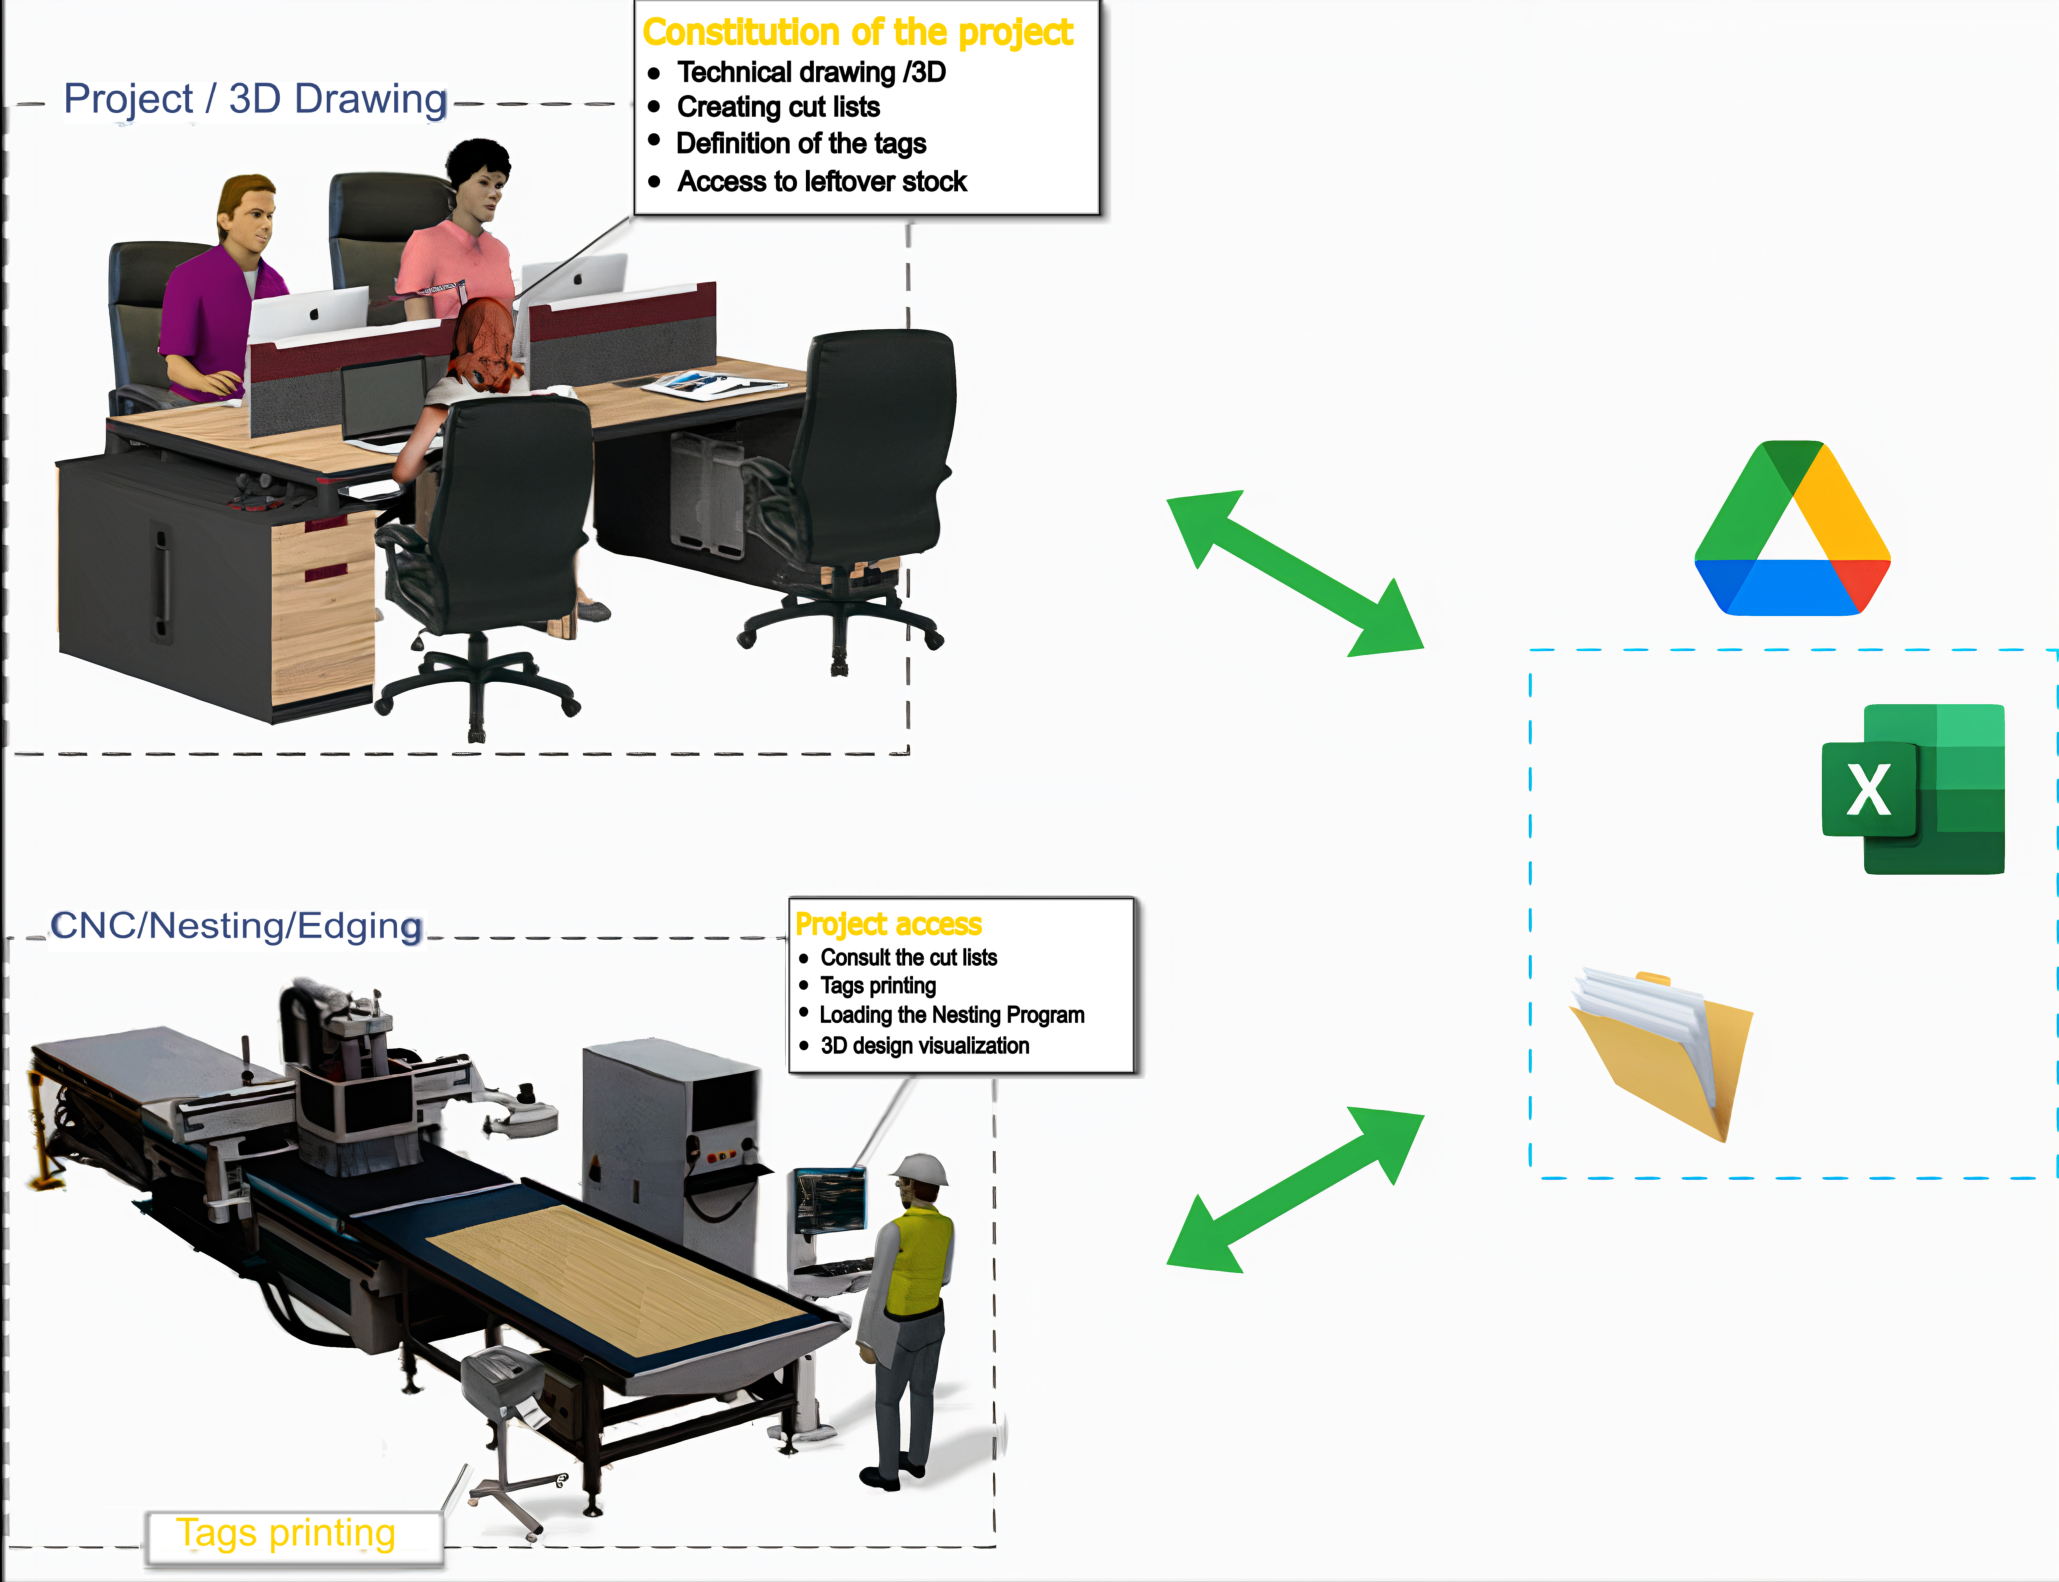
\includegraphics[width=.65\linewidth]{images/Development/chap4/MofreitasCaseIA.pdf}
    \caption{Graphical representation of how mofreitas initially accessed project information in different locations on the factory facility.}
    \label{fig:dataSharing}
\end{figure}

In particular, difficulties arise in situations where synchronization is not executed correctly, network failures occur, or obtaining specific project information becomes complex in an environment filled with data from other projects that are not immediately relevant to the operator. Therefore, handling this information requires a systematic and efficient approach to minimize the possibility of errors and improve the productivity of the production process.

The files produced by AlphaCAM\textsuperscript{\textregistered}, crucial for programming the nesting and CNC machines, are input into the corresponding control software for each machine and operated based on instructions provided by the operators. As mentioned earlier, these files, along with the identification labels that need to be affixed to the pieces after nesting, are accessible on all computers in the production area, located in a cloud-shared folder. Additionally, operators have the ability to consult and view each project in three dimensions by opening the files generated in SolidWorks\textsuperscript{\textregistered} using the eDrawing\textsuperscript{\textregistered} visualization software.


After the cutting and processing of each of the wooden components involved in the project, the assembly process begins, as shown in figure \ref{fig:shopFloor}. The purpose of this phase is to ensure that the furniture production has been carried out in accordance with the project specifications, thus minimizing errors at the final delivery location, which is often a significant distance from the initial manufacturing site.


\begin{figure}[ht!]
    \centering
    \includegraphics[width=.65\linewidth]{images/Development/chap4/mofreitas.png}
    \caption{The image illustrates the preliminary assembly stage at the Mofreitas furniture factory. Operators, among scattered components, check the correct fit of parts and completeness of furniture, essential before the subsequent packaging process. Source: \cite{noauthor_mofreita_2020}.}
    \label{fig:shopFloor}
\end{figure}

This phase often requires the use of various consumables such as screws, anchors, and glue, as well as a range of hardware including hinges, handles, and locks. In terms of inventory management, consumables are purchased from the warehouse by a designated operator in quantities that meet the demand. During this process, the operator is responsible for manually recording the description and quantity of items such as boxes of nails, screws, and other requisitioned items.

As for hardware, the list of materials associated with a specific project is directly processed by the warehouse manager. In this context, all these items are segregated into boxes and associated with the corresponding project through a reference code.

After the assembly, adjustment, and careful inspection of all furniture elements related to the project, the packaging phase begins. In this crucial stage, the components are securely packaged to ensure their integrity during transportation. They are also properly labeled, not only to ensure traceability and facilitate handling during transit but also to assist in correct assembly at the destination site. This labeling is of utmost importance as it contains detailed instructions and the assembly sequence, ensuring that the final assembly is carried out according to the project specifications and preventing the loss of components, which could cause significant logistical disruptions. This packaging process is meticulously planned and executed, aiming not only for the physical protection of the furniture but also for the optimization of space during transportation.

So far, we have covered the various phases of the production process related to the manufacturing of a specific furniture component at Mofreita's carpentry. This journey begins with the project proposal and culminates in the final product, already installed at the customer's location. Among the subprocesses that are essential for the smooth operation and consolidation of this production chain, inventory management stands out.

Primary difficulties are identified in two areas: the first concerns the logistics associated with consumables and hardware, and the second relates to the traceability of wood waste generated from the cutting lists. In terms of the first area, there is a pressing need to digitize the process of requisitioning consumables and hardware to avoid manual recording and to enable real-time integration of this information into the overall management process.

Additionally, the current management of inventory data is carried out using a generic spreadsheet, which hinders the automatic recording of time-related information associated with material inflows and outflows, as well as any price fluctuations. Therefore, updating the inventory management software is a crucial step towards modernizing the production process.

The proposed solution should not only facilitate the storage of inventory-related information but also enable the analysis of this data. This capability allows for the generation of statistics that can support more effective decision-making processes. Data such as the time interval between orders for a specific reference and the average delivery times from a particular supplier are of paramount importance. Given the inherent uniqueness of each project, it is only possible to establish a forecast for the production time. 

Regarding the production chain, the way raw materials are incorporated into the production line is the second issue. Specifically, the fate of the waste generated from each project and how this waste can be automatically reintegrated into the chain is a point of interest. Currently, there is no automatic update of information in the spreadsheet used for inventory control regarding the remaining raw materials from various cutting processes. The leftover wood boards throughout the workweek, which have a usable area, are manually rearranged and reintegrated into the storage area. Their subsequent use is determined by operators through visual inspection for a specific purpose. This operational method is sub-optimal as it results in more waste than if these leftovers were used in nesting processes.

Therefore, the goal is to adopt a strategy for tracking the remaining raw materials so that they can be automatically integrated back into the inventory for more efficient reuse in subsequent manufacturing projects. Specifically, for each waste piece, its dimensions, material type, thickness, and location on the shop floor are intended to be recorded. Additionally, it is crucial to know, if applicable, the wood grain direction. The solution to be developed in the context of Industry 4.0 should allow for the identification of each waste piece on the shop floor and its integration into the inventory list with all the aforementioned characteristics. This information should be utilized to further minimize raw material waste and make the entire process more efficient.


\section{The Software Architecture}\label{section:softwareArchitecture}

As established in the \textcite{ieee} standard, architecture is conceptualized as the fundamental organization of a system, embodied in its components, their relationships with each other and the environment, as well as the principles that guide its design and evolution. In this regard, the development of the software architecture for this project is crucial as it aims to build a system capable of performing a variety of functions simultaneously while adhering to essential criteria: scalability, security, traceability, interaction with a range of devices, and data distribution. This arrangement, by providing a broad spectrum of capabilities, contributes to a robust and versatile system that can adapt and efficiently respond to the variable and complex demands of the manufacturing environment.

\subsection{Scalability}\label{section:softwareArchitecture-scalability}
Scalability, characterized as the ability of a system to adjust its throughput according to emerging needs, expanding or reducing its performance \cite{garland2003large}, has been incorporated into the software architecture to ensure its future expandability and adaptability. These characteristics are particularly necessary in an environment that potentially receives data from sensors, machines, and microservices installed in the manufacturing ecosystem, as well as requests from external networks.

In order to integrate with existing internal services and potentially incorporate new services, specific technologies have been utilized. The \acrfull{fiware}\cite{fiware}, an open platform under the \acrfull{glp}\footnote{The GNU AFFERO GENERAL PUBLIC LICENSE Version 3  also know as General Public License (GPL) is a free software license that guarantees end users the freedom to run, study, share, and modify the software. It was created by the Free Software Foundation (FSF) \cite{tsai2008better}.} license, which provides a set of \glspl{api} that facilitate the development of intelligent applications, has been employed to enable system interoperability and efficient data handling. Additionally, Nginx\textsuperscript{\textregistered} \cite{nginx}, a high-performance web server, has been implemented to manage HTTP requests and load balancing, contributing to the scalability and reliability of the system. The Gunicorn, a Python \acrfull{wsgi} HTTP server\footnote{ WSGI is a specification that defines how web servers and web applications communicate in the Python ecosystem. It establishes a standardized interface that enables web servers like Gunicorn to effectively process requests from Python\textsuperscript{\textregistered} web applications \cite{eby2010pep}.  In other words, WSGI is not a server, a Python module, a framework, an API or any kind of software. It is just an interface specification by which server and application communicate \cite{clodoaldo2015}.}, was also used to serve the web applications of the system, enabling effective communication between the web application and the web server. Each of these technologies plays a vital role in optimizing the system architecture to meet the demands of scalability, adaptability, and integration.

Nginx\textsuperscript{\textregistered} is a widely adopted solution for web server and reverse proxy\footnote{Nginx acts as a simple proxy server, receiving HTTP requests from the client (acting as an HTTP server) and forwarding them to the backend server (acting as an HTTP client). There is therefore no new protocol or software involved. The mechanism is handled by the Nginx Proxy module \cite{fjordvald2018nginx}.}, recognized for its efficient load balancing capabilities in the context of network traffic distribution among multiple servers \cite{Chi2012}. Its Open Source version\footnote{Open-source software is characterized by granting users the right to access and modify the source code of the program, enabling customization according to individual user needs and the dissemination of the modifications made \cite{perens1999open}. This model has gained increasing support, with a growing movement in favor of open-source and a rising number of advocates engaged in this philosophy \cite{lerner2002}. } oferece o  algoritimo Round Robin\footnote{The term "round robin" originated from a historical practice of arranging signatures in a circular form to conceal the order of signing. It is believed to have derived from the French term "ruban rond" or "round ribbon" used in 17th-century France, where government officials signed petitions on ribbons attached to documents in a circular manner \cite[p. 716]{Hendrickson2008}.} for load balancing, which achieves a balanced distribution of incoming requests among the available servers \cite{nginxArticle}. When a client sends a request to the server, it acts as an intermediary, forwarding the request to one of the available backend servers. This approach is reinforced by maintaining persistent connections between the Nginx\textsuperscript{\textregistered} server and each backend server, allowing subsequent requests to be forwarded to the next server, taking into account its availability. Consequently, this strategy results in improved response times and a significant reduction in downtime \cite{Chi2012}.

In addition, load balancing provides redundancy and high availability, allowing the addition or removal of backend servers without interrupting ongoing services. The configuration exemplified in code \ref{code:nginx} demonstrates how the Nginx\textsuperscript{\textregistered} server can be easily set up to implement load balancing effectively \cite{nginxArticle}. For a clear visual understanding of this technology, figure \ref{fig:loadBalancing} offers a graphical representation that makes load balancing operation accessible and comprehensible.

\begin{lstlisting}[style=nginx, label={code:nginx}, xleftmargin=2.75em, language=nginx, caption={This configuration enables load balancing for the 'backend' service using Nginx. This allows to distribute incoming network traffic across multiple servers to improve performance, scalability, and reliability. The service is distributed in two other identical services running in parallel, ww40 and ww41.}, captionpos=b]
worker_processes auto;
http {
    upstream backend {
        server ww40;
        server ww41;
    }
    server {
        listen 80;
        location / {
            proxy_pass http://backend;
            # ... rest of the code.
        }
    }
}
\end{lstlisting}

\begin{figure}[ht!]
    \centering
    \includegraphics[width=.65\linewidth]{images/Development/chap4/load_balancing.png} 
    \caption{Load balancing is a widely used technique for optimizing resource utilization, maximizing throughput, reducing latency, and ensuring fault-tolerant configurations in web services. By distributing incoming HTTP traffic across multiple application instances, load balancing helps to evenly distribute the workload and improve overall performance. This allows you to efficiently proxy HTTP traffic to a group of servers, enabling scalability and high availability for your web applications. Source: \cite{nginx}.}
    \label{fig:loadBalancing}
\end{figure}

The software in question uses a Python-based \gls{api}. However, it is important to note that the Nginx\textsuperscript{\textregistered} server plays a distinct role, not being responsible for serving applications, but rather for redirecting HTTPS requests, serving static files, media files, caching, as well as load balancing, among other functionalities. To integrate the developed application with the web interface, an appropriate application server needs to be used.

On the other hand, Gunicorn\textsuperscript{\textregistered} is a software that acts as an implementation of the \acrfull{http} gateway interface (WSGI) for Python\textsuperscript{\textregistered} web applications. It plays an intermediary role between the web application and the web server, providing the functionality of an application server. This includes handling received HTTP requests, managing multiple worker processes, and properly routing requests to the corresponding \acrfull{wsgi} application \cite{chesneau2017gunicorn}. However, it is important to note that Gunicorn\textsuperscript{\textregistered} is not a complete web server like Nginx\textsuperscript{\textregistered} or Apache\textsuperscript{\textregistered}. Instead, it is designed to work in conjunction with a web server that can act as a reverse proxy and handle other tasks such as load balancing, serving static files, and providing advanced security features.

In a typical production setup, it is common to deploy Gunicorn\textsuperscript{\textregistered} together with a web server like Nginx\textsuperscript{\textregistered}. In this configuration, the web server handles incoming requests and forwards them to the application server processes. This combination provides a scalable and efficient architecture for delivering Python\textsuperscript{\textregistered} web applications, leveraging the specific capabilities of each component. This topology can be better understood in Figure \ref{fig:webArch}.

\begin{figure}[ht!]
    \centering
    \includegraphics[width=.65\linewidth]{images/Development/chap4/webArch.png} 
    \caption{Load .}
    \label{fig: webArch}
\end{figure}

Integrated into the development of the project at hand, \acrshort{fiware}\textsuperscript{\textregistered} serves as an additional set of software that enables scalability. This open-source platform, meticulously designed to drive solutions in domains such as smart cities, smart factories, smart agri-food, smart supply chain, among others, aims to create a unified and scalable system encompassing various IoT devices and communication services \cite{fiware}.

Scalability stands out in \acrshort{fiware}\textsuperscript{\textregistered}, a property derived from its architecture designed to smoothly adapt to an increasing number of connected devices and growing demand for services. From this perspective, the platform is capable of processing large volumes of data from different devices, allowing real-time ingestion and processing. Such capability becomes indispensable for applications that require quick and accurate responses.

Complementing its approach, the platform utilizes the robust \acrfull{ngsild} API, designed to standardize communication among a multitude of IoT devices. The underlying purpose is to facilitate communication and integration of devices within a cohesive ecosystem. This API is based on the \acrshort{ngsild} standard, which establishes a semantic data model for structured representation of entities and their attributes \cite{etsi2023}.

The motivation behind the creation of this software resided in the need to deal with the increasing complexity and diversity of connected devices in an integrated ecosystem. As more devices are incorporated into this ecosystem, there arises a demand for a standardized communication model that can facilitate effective and semantic information exchange. The API offers advanced features such as semantic queries, service discovery, and real-time notifications, enabling efficient and flexible communication among devices.

In summary, scalability stands out as one of the key advantages of \acrshort{fiware}\textsuperscript{\textregistered}, solidifying its ability to handle the continuous growth of \acrfull{iot} devices and data while providing the flexibility to incorporate new components and services as needed. This attribute cements the platform as a viable option for large-scale IoT implementations in environments that are constantly evolving.

\subsection{Security}\label{section:softwareArchitecture-security}

In the modern factory environment, security is of utmost importance. With the prevalence of cyber-attacks, a robust authentication system has been implemented to ensure the security of data for both internal and external users. Thus, this topic is a crucial factor considered in this project. External users access the developed platform through the Python\textsuperscript{\textregistered} WSGI application, which is built on the Django\textsuperscript{\textregistered} framework \cite{django}. The framework is widely recognized for its robust and comprehensive security system, which provides multiple layers of protection to ensure the security of the developed applications \cite{duisebekova2021django}. Additionally, the framework utilizes a robust \acrfull{orm}\footnote{\acrfull{orm} is a methodology and mechanism that allows object-oriented systems to securely store data in a database using models and constraints, instead of writing specialized code to interact with the database. This approach is particularly useful in web applications, which are multi-threaded and prone to race conditions. The concept of \acrshort{orm} was first introduced in the Hibernate project and has been widely adopted in other technologies, such as Microsoft's Entity Data Model for .NET systems  \cite{Elizabeth2008}.},  that contributes to the consistency and security of the data stored in the database \cite{duisebekova2021django,django-docs}. This combination of technologies provides a secure environment for processing and handling sensitive information in the application.

The developed application implements a comprehensive security system. It features an internal authentication server responsible for verifying the authenticity of external users registered in the system. Additionally, various protective measures are adopted to ensure the security of the application. Automatic input data sanitization and the use of prepared statements for database queries are examples of these measures, aimed at preventing the execution of malicious commands and the insertion of unwanted scripts into web pages.


Furthermore, the developed software offers a flexible authentication system that allows the implementation of different authentication methods such as login and password, token-based authentication, and time-limited key for password reset and user account activation. In conjunction with the Throttling system\footnote{Throttling is employed to govern the rate at which client requests are permitted, taking into account the originating IP address. By imposing temporary restrictions on request rates, Throttling serves the purpose of preventing abuses and server overload. It ensures a balanced allocation of server resources by limiting the frequency of requests made by a particular client \cite{drf-docs}.}, In addition, the developed software offers a flexible authentication system that allows the implementation of different authentication methods such as login and password, token-based authentication, and time-limited key for password reset and user account activation. Together with the Throttling system that controls the rate of user requests, these authentication measures ensure security and proper access control in the application. Furthermore, granular permissions are applied to control users' access to specific application resources. These permissions are defined based on roles and assignments of each user, ensuring that only authorized users have access to specific functionalities and data. Combined, these authentication measures, Throttling, and granular permissions contribute to comprehensive application security, protecting it against potential threats and ensuring strict access control.

Protecting sensitive data is another important factor. Password encryption using the BCRYPT \footnote{BCRYPT is a key derivation function for passwords that is based on the Blowfish cipher. It incorporates a salt to protect against rainbow table attacks and is an adaptive function, allowing the iteration count to be increased over time for increased security. This function is widely used as the default password hash algorithm in systems such as BSD. The hash string for BCRYPT includes the cost parameter, a salt, and the hash value. It provides a secure and efficient method for hashing passwords and protecting sensitive user data \cite{sriramya2015providing}.} algorithm. This is used to prevent storing passwords in plain text in the database, ensuring an extra level of security for user information. Additionally, Django\textsuperscript{\textregistered} has features for protection against Cross-Site Request Forgery (CSRF), an attack technique that exploits the browser's trust in requests made on behalf of the authenticated user \cite{django-docs}. These measures contribute to the integrity and confidentiality of the data handled by the application.

\subsubsection{Authentication System}
\label{subsubsection:Authentication}
The authentication system of the WSGI application adopts an HTTP-based approach and follows the communication flow of the OAuth2 protocol. In the specific context of the first authentication flow, there is a direct interaction between the web application and WSGI. In this process, the web application sends the user's credentials to the WSGI application's authentication provider using the "Password credential" authentication flow. This step is essential to verify the user's identity and ensure secure access.

After successful authentication, the \acrshort{wsgi} application is able to identify the user and obtain an authentication token from the Keyrock Identity Manager (IDM). This token is acquired through the client credentials flow, providing a secure way to access resources available in the \acrshort{fiware}\textsuperscript{\textregistered} environment. To ensure the integrity and validity of this token during resource access, the Willma software comes into play. This software acts as a layer of protection and control, playing a crucial role in protecting sensitive and internal resources within the \acrshort{fiware}\textsuperscript{\textregistered} ecosystem, through the role of \acrfull{pep}\footnote{PEP stands for Policy Enforcement Point. It is a component or system that is responsible for enforcing and implementing various policies within a specific context. The exact nature of the policies can vary depending on the domain or application in which the PEP is deployed. The PEP acts as a control point, intercepting and regulating incoming requests or actions based on the defined policies. It ensures that the specified rules and regulations are adhered to and enforced within the system, providing an additional layer of security and governance \cite{mont2006}.}.  It verifies the requests before directing them to the internal service network of \acrlong{fiware}, ensuring that only authenticated and authorized requests have access to the resources. Thus, the OAuth2-based authentication system, together with the "Password credential" authentication flow and the Willma PEP\textsuperscript{\textregistered}, provides a secure and reliable solution to control access to\acrshort{wsgi} application resources and ensure the protection of sensitive user data.


\begin{figure}[ht!]
    \centering
    \includegraphics[width=.65\linewidth]{images/Development/chap4/oauth.png} 
    \caption{The photo illustrates the authentication system. Using the OAuth2 flow, the application sends the user's credentials to the WSGI authentication provider, enabling authentication. Next, an authentication token is obtained from IDM Keyrock through the client credentials flow, allowing access to \acrshort{fiware} environment resources. A \acrshort{pep} component verifies and authorizes requests before forwarding them to \acrshort{fiware}'s internal service network, ensuring the security and integrity of sensitive data.}
    \label{fig: oauth}
\end{figure}


\subsection{Traceability}\label{section:softwareArchitecture-traceability}

The ability to track information plays a crucial role in various scenarios, particularly when it comes to statistical data analysis and pattern identification. In this context, the implemented system meticulously records all operations performed, allowing users to revisit and analyze these operations later on \cite{Marquesone}. This system makes use of two software components integrated into the FIWARE ecosystem: Orion-LD\textsuperscript{\textregistered} and Mintaka\textsuperscript{\textregistered} \cite{mintaka}. The former is responsible for instantly storing the current state of the entities involved in information transactions, while the latter maintains a complete history of all operations related to a specific entity. The following code snippet provides a clearer visualization of how this process works. This feature enhances transparency, facilitates error detection, and improves decision-making based on data.

To enable persistence and retrieval of historical context data, the NGSI-LD temporal interface is employed, with the Mintaka software playing a fundamental role. This interface allows context data to be represented as a series of data points, each with its respective timestamp. Each data point reflects the state of entities at different moments, enabling the analysis of statistics and trends.

Within the addressed ecosystem, there are two common approaches to trend data analysis. The first is the activation of the temporal interface, which enables the registration of all entities in the temporal database, regardless of the specific interest in each one. The second approach involves subscribing to individual entities and storing them in a time series database, such as QuantumLeap. The choice between these mechanisms should consider the specific system architecture as well as aspects related to disk space and HTTP traffic \cite{fiware_temporal_nodate}.

In the current project, due to the large number of entities that can be created and stored, the subscription methodology was adopted. This approach allows for the persistence of only the subscribed entities, i.e., those of specific interest, resulting in disk space savings. If the option to use the temporal interface were chosen, all entities would have their data registered in the temporal database, even those that are not relevant for the analysis at hand.

To illustrate this methodology, we can use the example of creating an entity of type "PART" with the name "LEG". This entity has an attribute with an initial value of "Left Leg", which was later changed to "Right Leg". Thus, by using a temporal subscription on this property, the "observedAt" attribute indicates the moment when the change occurred. The following code (\ref{code:temporalOutput}) exemplifies the addition of the attribute in the process:

\begin{lstlisting}[style=linux, label={code:temporalInput}, captionpos=b,  caption={Neste exemplo, é feita uma solicitação PATCH para atualizar a entidade "Part" com o identificador "LEG". O atributo "partName" é alterado para "Right Leg" e o atributo "observedAt" é adicionado com o valor "2023-05-18T10:00:00Z", indicando o momento em que a alteração ocorreu.}]
curl --location --request PATCH 'https://woodwork4.com/api/v1/part/urn:ngsi-ld:Part:LEG_LEFT/' \
--header 'Content-Type: application/json' \
--header 'Authorization: Bearer *' \
--data '{
      
    "partName": {
        "type": "Property",
        "value": "Right Leg",
        "observedAt": "2023-05-18T10:00:00Z"
    }
   
}
\end{lstlisting}

As a result of this operation, the context data was stored persistently in the temporal database, ensuring consistent preservation of historical context information. This means that it is possible to access and query the complete history of the changes that occurred, providing a detailed and accurate view of the context over time.

\begin{lstlisting}[language=json, label={code:temporalOutput}, caption={The outcome achieved following the formal request made to the temporal provider for the entity's change history in JSON format.}, captionpos=b]
{
    "id": "urn:ngsi-ld:Part:LEG_LEFT",
    "type": "Part",
    "partName": [
        {
            "type": "Property",
            "value": "Right Leg",
            "observedAt": "2023-05-18T10:05:00Z",
            "instanceId": "urn:ngsi-ld:attribute:instance:15d6640c-f726-11ed-8724-0242"
        },
        {
            "type": "Property",
            "value": "Left Leg",
            "observedAt": "2023-05-18T10:00:00Z",
            "instanceId": "urn:ngsi-ld:attribute:instance:3f9cd000-f726-11ed-851b-0245"
        }
    ]
}
\end{lstlisting}

Furthermore, in order to provide a more insightful visualization of the system architecture and the synergy between the previously mentioned features, the following illustration is presented, outlining the structure of the implemented system. The graphical representation highlights the interconnection between the Orion-LD and Mintaka components, as well as the use of the NGSI-LD temporal interface for the persistence and retrieval of historical context data. This visual representation aligns with the intention of offering a comprehensive understanding of the system's architecture and information flow, primarily emphasizing its remarkable traceability and trend analysis capabilities.

\begin{figure}[ht!]
    \centering
    \includegraphics[width=.65\linewidth]{images/Development/chap4/Temporal.pdf} 
    \caption{Architecture of the implemented system showcasing the integration of Orion-LD and Mintaka components, along with the utilization of the NGSI-LD temporal interface for persistence and retrieval of historical context data.}
    \label{fig: oauth}
\end{figure}

In summary, traceability plays a crucial role in statistical data analysis and pattern identification. The implemented system diligently records all operations performed, allowing users to revisit and analyze these operations later on. This is made possible through the integration of Orion-LD\textsuperscript{\textregistered} and Mintaka\textsuperscript{\textregistered} software within the \acrshort{fiware}\textsuperscript{\textregistered} ecosystem. Leveraging the NGSI-LD temporal interface, the temporal signature software maintains a complete history of operations, enabling analysis of statistics and trends. The methodology of data signing was adopted to persist only the entities of interest, thus saving disk space. This process enhances transparency, facilitates error detection, and improves data-driven decision-making by providing a detailed and accurate view of the context over time.

\subsection{Data Sharing}\label{section:softwareArchitecture-data_sharing}
The sharing of data plays a fundamental role in the project at hand. With the need to track processes, physical components, and files related to projects, it is crucial to have a system that enables the sharing of different types of information. Additionally, it is essential for the system to be scalable to accommodate future modifications, such as the addition of information from various IoT devices in the factory environment.


\subsubsection{Sharing Context  Data}
For these reasons and based on the considerations mentioned earlier, the FIWARE\textsuperscript{\textregistered} platform has been selected to integrate this project. In addition to enabling the scalability of new sensors in the existing infrastructure, the platform offers the capability to share context information in a semantic manner. This implies that information can be shared between different systems or devices without loss of meaning.

In the case of the FIWARE\textsuperscript{\textregistered} platform, the Orion-LD General Enabler plays a key role, being responsible for managing the context information. This information can be accessed through the NGSI-LD API, which uses the JSON-LD\footnote{JSON-LD is an advanced extension of the JSON (JavaScript Object Notation) format that significantly enhances the ability to represent and connect structured data on the web. This extension allows for the addition of semantic context to the data, resulting in the expression of information using shared terms and vocabularies. This approach promotes interoperability and simplifies seamless integration between various systems and applications \cite{Lanthaler2012, sporny2020json}.} (JSON for Linked Data) format for data representation.

JSON-LD is an extension of JSON\footnote{JavaScript Object Notation (JSON) is a versatile and efficient data interchange format. As a lightweight and text-based language-independent format, JSON was initially derived from the ECMAScript Programming Language Standard. It provides a concise and portable way to represent structured data by defining a minimalistic set of formatting rules. JSON enables seamless data exchange and integration across various platforms and programming languages \cite{rfc7159,pezoa}.} that allows adding semantic context to the data. This approach ensures that the information shared through the NGSI-LD API is enriched with additional meaning, facilitating its understanding and making it interoperable between different systems. In other words, the information is not simply transmitted, but is also associated with specific context and meaning. This feature allows for more advanced processing of the information, resulting in deeper analysis and more accurate decision-making.

To better illustrate this concept, consider an object called "car" being shared between two distinct ecosystems. If the context that defines the meaning of the term "car" is the same in both systems, there will be a consistent understanding of the object. This approach enriches data sharing, avoiding interpretation issues in communication between diverse devices.

\begin{figure}[ht!]
    \centering
    \includegraphics[width=.65\linewidth]{images/Development/chap4/jsonld.pdf} 
    \caption{This figure shows JSON-LD’s data model, a Linked Data graph. Source: \cite{Lanthaler2012}}.
    \label{fig: jsonld}
\end{figure}

The figure \ref{fig:jsonld} clearly illustrates the concept of Linked Data, where objects serialized in JSON format are associated with a "subject". For example, a JSON object with the name "car" has a specific meaning for a person. However, for a machine, it is just a sequence of characters. When the "subject" is introduced and associated with an object, machines communicating in this ecosystem recognize that a "car" has specific attributes associated with it and that all objects of the same type within this ecosystem have similar characteristics. This allows machines using this data sharing method to consistently and standardizedly recognize the information.

Based on these principles, it is possible to send project information to the Context Broker using a specific semantic. This means that all entities and attributes shared among devices within this context will be interpreted in the same way. This uniformity of understanding ensures that data is transmitted and understood consistently, facilitating communication between different components of the system and enabling more precise and reliable analysis. In summary, the use of a specific semantic in information sharing ensures the harmonization and common understanding of each entity and its attributes, optimizing the process of data exchange and analysis.

\subsubsection{Sharing Project Data}\label{subsubsection:SharingProjectData}

One fundamental aspect of the system in question lies in its ability to share crucial project files across the entire development environment, encompassing both the project engineering team and the operators on the factory floor. File exchange should occur through a web interface as well as access to files in the file system of each computer or mobile device used by company users. Among the types of shared files, CAD drawings, CNC commands, project images, and spreadsheets are particularly noteworthy. These records contain technical information and important details to ensure the proper execution of the project, and it is essential to have access to them by different production departments.

Furthermore, one of the fundamental premises in this approach is the need to design a solution based on open-source technologies combined with proprietary software. This requires careful harmonization between leveraging open-source tools and resources and implementing custom systems to meet specific requirements related to file sharing in the project context. This approach aims to take advantage of the benefits offered by open-source technologies, such as flexibility, transparency, and collaboration, while also enabling integration with proprietary systems to meet the specific demands of file sharing in this context.

To meet the needs of sharing crucial files in the development environment, project engineering, and factory floor, a comprehensive software architecture was designed, encompassing various essential services. Among these services, the Syncthing, Nginx, Web Platform, and File Watcher stand out, and their integration is visualized in figure \ref{fig:supervisor}.

\begin{figure}[ht!]
    \centering
    \includegraphics[width=.65\linewidth]{images/Development/chap4/Superviser.pdf} 
    \caption{Visual representation of the architecture for file sharing: an integrated solution that allows the efficient exchange of information between different systems and devices, guaranteeing the necessary security, scalability and interoperability.}.
    \label{fig: superviser}
\end{figure}

The Nginx server plays a prominent role, performing multiple vital functions for the system. In addition to acting as a load balancer and reverse proxy server, Nginx is also used as a web server. This versatility allows it to be employed in serving media files in a specific web application. In this context, a custom web platform was developed to interact with the WW4 API, which is responsible for receiving and storing files uploaded by users. Relevant information about the file locations is properly recorded in a database, enabling access to this information from the corresponding web page.

However, to enable access to files present in each user's file system, the strategy of using Syncthing was chosen. Syncthing is a decentralized and open-source file synchronization platform designed to enable secure, reliable, and private sharing and synchronization between network-connected devices. Unlike centralized cloud storage services, Syncthing does not rely on external or intermediary servers for file storage. Instead, it adopts a peer-to-peer approach, where devices connect directly to each other for data synchronization. This approach ensures that files remain under the control of users, giving them greater privacy and control over shared data. Syncthing is compatible with a wide range of platforms, including Windows, Mac, Linux, Android, among others, allowing file synchronization across diverse devices regardless of the operating system used. Additionally, this platform offers advanced features such as end-to-end encryption, real-time change detection, and automatic conflict resolution.

In the adopted strategy, the use of Syncthing on the server allows monitoring the same folder that receives information from the web application. This configuration ensures the synchronization of the information entered by the web application on the computers of each user sharing the same directory through Syncthing.

However, to enable the reverse flow, that is, when the user uploads files to their shared folder and these changes are reflected in the API, it is necessary to implement a file monitoring system on the server. For this purpose, a program was developed that operates simultaneously with the API and monitors events occurring in the file system. This program is called the File Watcher. This structure allows the creation, deletion, or updating of files or folders based on the type of event that occurs. The following figure illustrates the logic behind this created file supervisor.

\begin{figure}[ht!]
    \centering
    \includegraphics[width=.95\linewidth]{images/Development/chap4/FileWatcher.pdf} 
    \caption{Logic used to create the file supervision system}.
    \label{fig: fileWatcher}
\end{figure}

\section{Data Model}\label{section:dataModel}

The development of a data model is crucial for the efficient management of processes involved in the furniture industry \cite{Batra1995}. In the scope of the furniture industry, the data model provides a structured representation of the information required for furniture manufacturing, enabling efficient storage, retrieval, and manipulation of this data.

As mentioned in section \ref{section:conceptulaDataModel}, the first phase of data model development involves identifying the key components and attributes necessary in the furniture manufacturing process. This includes data about wood types, piece dimensions, individuals involved, required manufacturing operations, among others.

Each piece of information in the data model is characterized as an entity. These entities are interconnected through relationships, which express the dependencies and interactions between different entities. For example, an entity called "Part" may have a relationship with multiple "Work Task" entities, which represent the work performed by an operator on a piece of wood, and which in turn also have a relationship with a machine. Such a relationship between entities is called many-to-many, and as a result, a third entity is needed to connect the two entities \cite{fiware_entity_relationship}. In this context, the "Work Task" entity acts as a linking table, also known as a bridge table.\footnote{A bridge table, also known as a join or map table, is a database design pattern used to resolve many-to-many relationships between entities. It acts as an intermediary, containing primary keys from each linked table, and uniquely binds records from these tables. Unlike a fact table, the bridge table enforces a mandatory relationship, restricting data based on records from another subject area. Benefits include joining and filtering data streams from each side of the bridge, and preventing double counting \cite{international_business_machines_corporation_ibm_2023}. }. In this way, it is possible to establish more complex relationships between elements, considering that one operator can work on multiple parts, and a part can have multiple operators performing various processes on it. Figure \ref{fig: WorkTask} illustrates this process.


\begin{figure}[ht!]
    \centering
    \includegraphics[width=.65\linewidth]{images/Development/chap4/Example WorkTask.pdf} 
    \caption{Simplified representation of the relationship between a piece of furniture and the work performed by the worker.}
    \label{fig: WorkTask}
\end{figure}


Moreover, it is important to model not only static information but also the processes and operations involved in the manufacturing. This includes information about the sequence of operations, operation times, machines and tools used, among others. These pieces of information can be modeled as attributes of the entities or as separate entities. The data model should also take into account the needs for traceability. For this purpose, it is useful to include unique identifiers for the parts, creation dates, start and end times, and other important entities.

In the process of developing the data model, emphasis was given to creating entities following reusability patterns, as well as adhering to the OpenAPI Specification (OAS) standards.\footnote{The OpenAPI Specification (OAS) provides a standardized, language-independent interface for HTTP APIs. It enables users and machines to understand and use a service without needing source code, documentation, or network traffic inspection. An OpenAPI definition serves various use cases, such as generating API documentation, producing servers and clients in diverse languages, and facilitating testing tools.}. Each data entity, within its particular context, may have variations depending on the specific use case. However, it is crucial that the common internal structure of each data entity is standardized to encourage reusability. In other words, despite the inherent uniqueness of each use case, the organization and structuring of data should adhere to a consistent pattern, which facilitates the reuse of these structures in different scenarios. Additionally, the development of the data model was carried out using the Fiware context generation pattern, to create context following the JSON-LD standard.

The data model that was developed can be viewed through the following GitHub link: \url{https://github.com/More-Collaborative-Laboratory/ww4zero}. Additionally, the context files that were generated during the development process are also available in this repository.

\section{Traceability of a Project}\label{section:project}

As mentioned in the methodology section of the project, which refers to section \ref{section:ProjectTraceability}, the traceability process begins after the project is approved by the client and the cutting lists are generated. The supervision software is then able to retrieve the data from these lists and, based on that data, send the part information to the server responsible for managing such information. The code developed for the program responsible for the supervision process can be found at \url{https://github.com/iaggocapitanio1/WWWatcher}. This is just one of the services involved in the traceability process.

An important element to highlight is file synchronization. The methodological aspect of this topic, along with the architectural issues involved, have been discussed earlier in sections \ref{section:fileSharing} and \ref{subsubsection:SharingProjectData}. It is worth noting that a crucial software for implementing this architecture is available in the GitHub repository at the following address: \url{https://github.com/iaggocapitanio1/WW4FileFinder}. This software is responsible for synchronizing what the server receives in its file system with the WW4 API.

\subsection{Dashboard Features}

In relation to project traceability, the ability to visualize relevant data is essential. As defined by \textcite{old2023}, a dashboard is characterized as a way to present valuable information about a business or can be understood as a web page that aggregates information, functions, and significant aspects of an object. In the context of this project, a user interface for proper data visualization would be crucial. However, creating this interface was not one of the objectives of this project, as this task was allocated to a third-party company working in parallel to this work. Thus, the main objective here is to analyze the characteristics that this software should have to provide a traceability system with relevant and objective information.

In the study conducted by the authors \textcite{YIGITBASIOGLU201241}, they emphasize the importance of flexibility in dashboards, allowing users to easily switch between different presentation formats. Additionally, the authors highlight the usefulness of pop-ups and alerts as tools that can assist users during their activities. Complementing this perspective, another research conducted by the authors \textcite{NADJ2020113322} emphasizes that dashboards, besides providing a broader perception of important events, are valuable instruments for strategic decision-making in companies, presenting the advantage of being simple and displaying crucial information for the business model.

In this sense, it is expected that the developed dashboard is capable of displaying the current status of ongoing projects, as well as relevant information such as approved pending projects, details of projects in progress, financial values involved, time spent for execution, and files of a project. These are just a few examples. Figures \ref{fig:dashboard01} and \ref{fig:dashboard02} provide a brief overview of the developed dashboard.

\begin{figure}[!ht]
 \centering
         \includegraphics[width=0.65\linewidth]{images/Development/chap4/dashboard_01.png}
         \caption{Dashboard intuitively showcasing the status of projects in a straightforward manner, with the added feature of filters.}
         \label{fig:dashboard01}
\end{figure}

\begin{figure}[!ht]
 \centering
         \centering
         \includegraphics[width=0.65\linewidth]{images/Development/chap4/dashboard_02.png}
         \caption{Dashboard showcasing the data related to a piece of furniture, which has been transmitted by the supervision software.}
         \label{fig:dashboard02}
\end{figure}


\section{Traceability of Leftover}\label{section:leftover}

In this section, the emphasis is on the practical process involved in implementing leftover traceability. The methodology related to this process has already been addressed in Section \ref{section:LeftoverTraceability}. At this point, the focus is on the practical development carried out to achieve the proposed objective. The corresponding Github repository can be accessed at the following address: \url{https://github.com/iaggocapitanio1/ObjectDetectionWW4}.

More specifically, Subsection \ref{section:leftover-image_processing} details the work done in terms of image processing. Subsection \ref{section:leftover-database_storage}, on the other hand, explains the image storage process. Finally, Subsection \ref{section:leftover-computer_vision} reports on the development done to classify leftover material using computer vision techniques.

\subsection{Image Processing}\label{section:leftover-image_processing}
In the current section, the aim is to clarify the development carried out to achieve automatic dimension detection of parts in the manufacturing environment. The detection process was performed using the Python programming language, with a special focus on the utilization of the OpenCV library \cite{opencv_library}. This library is widely known for providing a set of efficient tools and dedicated numerical implementations for image processing, which was crucial for the success of this task.

The code snippet \ref{code:imageProcessing} provides a simplified representation of the code developed to detect the dimensions of a part. Although simplified, the code exposes the main aspects of the process. For example, in line two, one can observe the implementation of the Canny filter, whose functionality was discussed in Section \ref{subsection:Canny-edge-detection}.

\begin{listing}[!ht]
\begin{minted}[
frame=single,
framesep=2mm,
baselinestretch=1.2,
fontsize=\footnotesize,
breaklines=true,
linenos
]{python}
def process_frame(frame: numpy.ndarray, name: str) -> Optional[Tuple[numpy.ndarray, Dict]]:
    canny_frame = cv.Canny(frame, threshold1=settings.THRESHOLD_MIN, threshold2=settings.THRESHOLD_MAX)
    dilatation = numpy.ones(settings.DILATATION_SIZE, numpy.uint8)
    dilated_frame = cv.dilate(canny_frame, dilatation, iterations=2)
    eroded_frame = cv.erode(dilated_frame, dilatation, iterations=2)
    contours, _ = cv.findContours(eroded_frame, cv.RETR_EXTERNAL, cv.CHAIN_APPROX_SIMPLE)
    ratio = get_ratio_pixels_millimeters(img=frame)
    for contour in contours:
        if cv.contourArea(contour) > settings.MIN_AREA_FILTER:
            clean_contour_points = cv.approxPolyDP(contour, epsilon=0.01 * cv.arcLength(contour, True), closed=True)
            processed_frame = cv.polylines(frame.copy(), pts=clean_contour_points, isClosed=True, color=(255, 0, 0), thickness=12, lineType=cv.LINE_AA)
            bbox = get_bounding_box(img=processed_frame, corners=clean_contour_points, draw=True)
            return processed_frame, dict(bbox=dict(x=bbox[0], y=bbox[1], width=bbox[2], height=bbox[3]), corners=clean_contour_points.tolist())
    return None
\end{minted}
\caption{Snippet of code used to extract geometric information from a leftover piece.}
\label{code:imageProcessing}
\end{listing}

After applying the Canny filter, morphological operations of dilation and erosion are performed. These operations are intended to obtain a more uniform and continuous contour structure in the image. Dilation, which expands the white areas in the image, is used to fill gaps and connect separate objects, enhancing the representation of edges in the image. Subsequently, the morphological erosion operation is used to further refine the image's contours. Erosion, which involves reducing the white areas, aims to eliminate noise and separate connected objects, contributing to a more accurate representation of edges. The combined use of these two operations aims to achieve well-defined edges and remove possible discontinuities that may be present in the image. This sequence of operations is known as morphological closing and is often used to improve the quality of object edges in images and facilitate subsequent analysis \cite{Jia5555633}. An example of the application of these operations can be observed in Figure \ref{fig:erode}.

\begin{figure}[!ht]
     \centering
     \begin{subfigure}[b]{0.325\linewidth}
         \centering
         \includegraphics[width=0.95\textwidth]{images/Development/chap4/original.jpg}
         \caption{Original image}
         \label{fig:imageProcessingExampleA}
     \end{subfigure}
     \hfill
     \begin{subfigure}[b]{0.325\linewidth}
         \centering
         \includegraphics[width=0.95\textwidth]{images/Development/chap4/after-dilatation.jpg}
         \caption{Image after dilatation.}
         \label{fig:imageProcessingExampleA}
     \end{subfigure}
     \hfill
     \begin{subfigure}[b]{0.325\linewidth}
         \centering
         \includegraphics[width=0.95\textwidth]{images/Development/chap4/after-erode.jpg}
         \caption{Image after erode.}
         \label{fig:imageProcessingExampleB}
     \end{subfigure}
      \caption{A comparison of the image processing procedures using dilatation and erosion  operations.}
      \label{fig:erode}
\end{figure}


Prosseguindo com a análise, a função \emph{findContours} da biblioteca OpenCV é aplicada. Esta função é designada para identificar pontos que se encontram sobre uma linha de contorno. Notavelmente, a função apresenta a versatilidade de retornar todas as coordenadas identificadas ao longo de tal linha ou, alternativamente, apenas um par de pontos que define uma linha com o mesmo coeficiente angular. Esses objetivos podem ser alcançados através dos argumentos \emph{CHAI\_APPROX\_NONE}, \emph{CHAI\_APPROX\_SIMPLE}, respectivamente \cite{open_source_computer_vision_opencv_2023}. Especificamente, o uso do último argumento permite uma representação simplificada do contorno, retornando apenas os pontos que marcam uma mudança na direção do contorno. Essa configuração é visível no Código \ref{code:imageProcessing}. O resultado da aplicação da função pode ser visualizado na figura \ref{fig:findCountours}.

\begin{figure}[!ht]
 \centering
         \centering
         \includegraphics[width=0.65\linewidth]{images/Development/chap4/fullcorners.jpg}
         \caption{Vertices identified upon applying the findContours function. The marked points represent the accurate detection of contour vertices in the image.}
         \label{fig:findCountours}
\end{figure}

In the context of the analysis performed, the standard contour detection is not sufficiently accurate, as only the vertex points are of interest, and as can be seen in Figure \ref{fig:findCountours}, there is an excessive amount of points. To address this specificity, the Ramer-Douglas-Peucker (RDP) algorithm \cite{Soendoro6021584}, implemented in the OpenCV library as the \emph{approxPolyDP} function, is used. This function aims to simplify the representation of a contour by reducing the number of points that compose it, while preserving the overall shape of the analyzed object, depending on the epsilon value used. Epsilon represents the degree of simplification of the original curvature: larger values result in shapes further from the initial curvature, while smaller values maintain greater fidelity to the original shape \cite{minichino2015learning}, as illustrated in Figure \ref{fig:rdp}.


\begin{figure}[!ht]
 \centering
         \centering
         \includegraphics[width=0.65\linewidth]{images/Development/chap4/rdp.png}
         \caption{The image demonstrates the Ramer–Douglas–Peucker (RDP) algorithm, a technique that simplifies a curve by reducing redundant points, while preserving its overall shape. Adapted from: \cite{fabian_hirschmann_ramer-douglas-peucker_nodate}.}
         \label{fig:rdp}
\end{figure}

In this way, the \emph{approxPolyDP} function allows for simplifying the representation of contours, focusing primarily on the vertices. This approach not only improves the analysis but also preserves vital information from the image. The choice of an epsilon value corresponding to ten percent, which has shown satisfactory results and was also adopted by the author \textcite{minichino2015learning}, leads to obtaining an accurate and efficient vertex representation. This efficiency is evident in the subsequent image, where the vertex points are clearly delineated.

\begin{figure}[!ht]
 \centering
         \centering
         \includegraphics[width=0.65\linewidth]{images/Development/chap4/corners.jpg}
         \caption{Graphical representation of image corners obtained after the application of the Ramer-Douglas-Peucker algorithm. The highlighted points demonstrate the algorithm's efficiency in simplifying and accurately identifying vertices.}
         \label{fig:rdp}
\end{figure}

Moving forward in the analysis, a crucial step is to establish the relationship between measurements in pixels and real-world dimensions. In this regard, the authors \textcite{GARRIDOJURADO20142280} introduced a novel approach that involves implementing a fiducial model based on markers known as Aruco markers. These markers, due to their uniqueness, are easily recognized by algorithms. Each Aruco marker has a unique characteristic that enables the determination of the correspondence between pixels and millimeters.

With this valuable information, it becomes feasible to convert the distances recorded in pixels into metric units. This conversion is performed using Equation \eqref{eq:euclidian}, which calculates the Euclidean distance between two points. Therefore, by applying this equation, an efficient and accurate method is obtained to translate measurements in pixels into real-world dimensions, thus establishing an essential bridge between the digital image and the analyzed physical object. The result of this process can be observed in Figure \ref{fig:output}.

\begin{equation}
d(\mathbf{a}, \mathbf{b}) = \sqrt{(a_1-b_1)^2 + (a_2-b_2)^2 + \ldots + (a_n-b_n)^2}
\label{eq:euclidian}
\end{equation}
\begin{figure}[!ht]
 \centering
         \centering
         \includegraphics[width=0.65\linewidth]{images/Development/chap4/output.jpg}
         \caption{Illustration of the Euclidean distance calculation between two points. Each point corresponds to a corner obtained after applying the Ramer–Douglas–Peucker algorithm. The distance, represented by the line connecting the points, is calculated in pixels and subsequently converted into metric units for accurate physical dimensions.}
         \label{fig:output}
\end{figure}

In summary, the results of this image processing workflow demonstrate success in detecting object edges, simplifying complex contours to their vertices, and converting measurements from pixels to metric units. This method enables precise geometric analysis of objects in the image, highlighting the applicability of the presented information for the efficient detection of leftover dimensions through image processing.

\subsection{DataBase Storage}\label{section:leftover-database_storage}

The data collection and storage process begins with the acquisition of the image by the IDS camera sensors. In a subsequent step, this data is processed by the Jetson device. Finally, it is sent to the Mofreitas server for efficient storage. It is important to emphasize that the storage of this data on the server only occurs when the "confirmed" attribute of the image is marked as true. This criterion ensures that only relevant information is stored in the database, avoiding the creation of images that are not associated with leftovers on the server.

Going deeper into the analysis, after the identification of the geometric characteristics of the leftovers, this information is sent to the database system. The system is designed to store not only the dimensions of the leftovers but also additional essential information, such as the boundary box, which plays a vital role in the future training of a Convolutional Neural Network (CNN). However, due to the restriction imposed by the NGSI-LD API, which prohibits direct storage of binary files, the leftover images are directed to the WW4 API. This API has the dual task of, on one hand, storing the images in the server's file system, and on the other hand, creating a corresponding entity in the Orion-LD GE\textsuperscript{\textregistered}. Thus, an entity of type "leftover" is created that can be integrated into the FIWARE\textsuperscript{\textregistered} ecosystem. This results in a unified and efficient approach to the storage and manipulation of leftover data.

Next, a demonstration is presented of what is stored in the database, as illustrated in Code \ref{code:leftover-storage}. This code snippet reveals pertinent information that is retained, including corners (points identified in pixel units), the creation date, and the encoded identifier of the leftover. It is worth mentioning that the snippet also includes details for constructing a boundary box. Additionally, it includes the scale obtained in the measurement phase between the pixels of the image and their corresponding values in metric units. It is important to note that the coordinates are in GeoJSON format.\footnote{GeoJSON is a data interchange format for geospatial information, built on the foundation of JavaScript Object Notation (JSON). It's specifically tailored for representing a variety of geographical structures. These include points, lines, polygons, multipoints, multilines, and multipolygons, encapsulating the diverse shapes that geographical features can exhibit. Furthermore, it has the capacity to represent features that possess non-spatial properties, thereby enhancing its versatility. It utilizes the World Geodetic System of 1984 (WGS84) as its geographical coordinate reference system. This system is a globally recognized standard for geodesy, cartography, and navigation. The units of measure employed by GeoJSON are decimal degrees, aligning with the common conventions for latitude and longitude representation \cite{butler2016geojson}. }, A key feature of the GeoJSON format is its ability to allow the web application to extract relevant information about the leftover, such as angles and areas. This particularity of the GeoJSON format makes it easy to manipulate by various frontend libraries, such as the LeafLet library \cite{paullecam_paullecamreact-leaflet_nodate}. 

\begin{listing}[!ht]
    \begin{minted}[frame=single, framesep=2mm, baselinestretch=1.2, fontsize=\footnotesize, linenos, breaklines]{json}
[
    {
        "id": "leftover_am9gkLB9We7bQD4Z",
            "url": "http://193.136.195.25/ww4/api/v1/storages/leftover/leftover_am9gkLB9We7bQD4Z/",
            "created": "2023-05-29T04:14:33.632861Z",
            "modified": "2023-05-29T04:14:33.632935Z",
            "file": "http://193.136.195.25/media/internal/leftovers/images/default/image_ayAkgDz.jpg",
            "corners": {
                "type": "Polygon",
                "coordinates": [
                    [510, 422],
                    [510, 480],
                    [567, 481],
                    [567, 423],
                    [510, 422]
                ]
            },
            "treated": false,
            "confirmed": true,
            "x": 510.0,
            "y": 422.0,
            "width": 57.0,
            "height": 145.0,
            "thickness": -1.0,
            "ratio": 1.1500877,
            "klass": "Oak",
            "batch": "default",
            "location_x": 0,
            "location_y": 0
    }
]
\end{minted}
\caption{JSON representation storing comprehensive details of a leftover piece.}
\label{code:leftover-storage}
\end{listing}

\cleardoublepage
\chapter{Results and Discussions}\label{cap:results}


 \section{System Analysis and Architecture Proposal}\label{section:systemArch}

The focus of this section is to examine the suggested architecture for the system and the achieved results. The design of the system structure aims to effectively track the information related to both leftovers and furniture projects. The code with all services developed for the architecture are in the appendix \ref{apendice3}.

Furthermore, it is crucial that the system is capable of sharing the specific data linked to each project. With this vision in mind, a robust backend service was developed, whose main function is to provide relevant information about the projects and leftovers.

Additionally, an important aspect of the proposal is the security of access to the information. This ensures that only authorized users can access confidential data, preserving the integrity and confidentiality of the information managed by the system.

\subsection{Security}
As smart factories become increasingly prominent in the current era, the emphasis on corresponding cybersecurity increases exponentially \cite{Ervural2018}. Given this context, this section aims to present the achieved results regarding protection against cyber-attacks for the developed system.


\subsubsection{Code Injection Threats}

Code injection attacks are among the most common practices that compromise the security of web applications \cite{Ray10.1145/2103656.2103678}. These threats occur through the insertion of malicious commands, which can alter or compromise the integrity of the information stored in databases. Although these attacks are most commonly associated with SQL applications, NoSQL applications are not exempt from these risks. As evidenced by \textcite{ron2015no}, a PHP application using MongoDB as a database can be susceptible to these types of attacks, highlighting potential security vulnerabilities.

The application developed in this work is robust against code injection attacks. As reported by \textcite{etsi2023}, the Orion-LD Context Broker, which is an integral part of this application, provides protection against such threats. This is achieved by prohibiting certain characters in any part of the payload.

This security strategy helps ensure that malicious commands cannot be injected, thus increasing the security of the stored data.

Despite the system developed in this work also using an SQL database, which could represent a potential point of vulnerability, security measures have been implemented to mitigate these concerns. In particular, the use of an Object-Relational Mapping (ORM) adds a layer of protection against code injection attacks. More specifically, the application using this type of database is built with the Django framework. Studies conducted by \textcite{duisebekova2021django} have shown that Django is resilient to such attacks. Furthermore, the official documentation of the framework also emphasizes that Django is secure against code injection attacks \cite{django-docs}.

Therefore, the system is secure against this type of cyber attack.

\subsubsection{Availability}
Availability refers to the continuous and timely accessibility of information whenever needed, whether by a user or the device itself. In this regard, Internet of Things (IoT) resources need to be readily accessible to meet demands or prevent significant losses. This assurance of constant and real-time access is a fundamental component in the efficient structuring of IoT systems \cite{Ervural2018}.

In this context, a potential threat to system availability is a Denial-of-Service (DoS) attack, a tactic that involves overwhelming a device by continuously sending data in high volume and short intervals. Such an attack can force the device to process an excessive amount of non-essential data, potentially leading to its inability to function properly. Despite the enhanced resilience of modern devices, mitigating DoS attacks often involves identifying and blocking the attacker's source address on the network, a process that can be automated through intelligent algorithms \cite{DUKE20024}.

The application developed in this work provides an effective barrier against DoS attacks. This is enabled by the fact that the application was built using the Django Rest Framework (DRF), which incorporates a flow control system known as Throttling. This system allows limiting the number of requests received from each IP address, serving as a protective measure against the request overload characteristic of DoS attacks \cite{drf-docs}. Additionally, a restriction on the payload size has been implemented to avoid overwhelming the web server, especially to counter attacks such as Packet Overflow Denial (POD) attacks\footnote{Packet Overflow Denial (POD) is a cyber security attack that can be modeled for Internet of Things (IoT) networks \cite{abdollahi_intrusion_2020}, exploiting the limited computational resources of conventional IoT devices. In this attack, malicious actors intentionally increase the length of transmit packets, leading to degradation of network resources \cite{acharya2016intrusion}.}. Thus, there is mitigation against this type of attack by denying requests that overload the system's computational resources.
\begin{listing}[!ht]
\begin{minted}{python}
DATA_UPLOAD_MAX_MEMORY_SIZE = mega_bytes_to_bits(mega=50)
REST_FRAMEWORK = {
    'DEFAULT_THROTTLE_CLASSES': [
        'rest_framework.throttling.AnonRateThrottle',
        'rest_framework.throttling.UserRateThrottle'
    ],
    'DEFAULT_THROTTLE_RATES': {
        'anon': '100/day',
        'user': '5000/day'
    },
    # other configurations 
}
\end{minted}
\caption{This code snippet illustrates the configuration for implementing throttling and limiting the payload size to 50 megabytes in Django Rest Framework.}
\label{lst:throttle_config}
\end{listing}

Another possible type of attack is \acrfull{ddos}. DDoS attacks represent a significantly more insidious threat, where the attacker can remain relatively anonymous while causing considerably more harmful impact. In this type of attack, malicious code is created and spread to infect multiple machines on the Internet. When activated, this code initiates attacks from all or some of the infected machines. Some variants of these attacks monitor public sites on the Internet and automatically initiate when a specific keyword is detected, making it extremely difficult to trace the attacker. This approach is concerning as a commonly used keyword can trigger an attack even without direct action from the attacker. The intention behind these tools is clearly cyber terrorism. In summary, DDoS attacks distribute the assault among various machines that have been contaminated with malicious software, making tracking the attacker a considerable challenge.

The system developed in this work is equipped with robust mechanisms such as Throttling and Load Balancing, both effective in mitigating \acrshort{ddos} attacks. Throttling controls the number of requests a single IP can make, while Load Balancing evenly distributes network traffic among multiple servers, avoiding the overload of a single server. These features enhance the system's resilience against DDoS attacks, reducing its susceptibility. However, it is important to note that while such measures can mitigate the effects of these attacks, they do not eliminate them entirely. DDoS attacks are complex and continually evolving, requiring constant vigilance and frequent security updates to maintain the system's robustness.

\subsubsection{Integrity}

Data integrity is a crucial aspect of ensuring application security. It is necessary to ensure that only authorized users can access and manage the resources they are granted permission to. In this context, the WW4 API plays a fundamental role in managing the resources provided to the web application. It offers the ability to manage resources using the Role-Based Access Control \acrfull{rbac} model. This model allows defining roles and permissions for users, controlling their access to resources based on their specific function within the application. This way, data integrity is preserved, ensuring that only authorized users can interact with resources and perform appropriate actions, reinforcing the security of the application.

\begin{figure}[!ht]
    \centering
    \includegraphics[width=0.65\linewidth]{images/chap5/RBCA.pdf}
    \caption{Illustration of resource access in the system according to the user's role type, following the \acrfull{rbac} model.}
    \label{fig:RBAC}
\end{figure}

Therefore, by adopting measures such as Role-Based Access Control (RBAC), the system effectively ensures the security and integrity of data. This is achieved by limiting and regulating access to system resources based on user roles. As a result, only authorized users can interact with relevant data and perform permitted actions. These restrictions not only strengthen the application's security but also contribute to maintaining data integrity.

\subsubsection{Authentication}

In addition, a security system based on access tokens has been implemented, utilizing JWT encoding\footnote{The JSON Web Token (JWT) is an advanced construct embedded within a JSON object, carefully defined according to the specifications of RFC 7519 \cite{johns_2016}. It serves as a secure channel for the transfer of a collection of information between two distinct parties. This mechanism provides a solid method for data transmission, notable for its verifiability and reliability, attributes that arise from its inherent ability to be digitally signed \cite{Ahmed9022766}.}. This encoding system is more flexible than using session cookies, as the process of verifying access permissions to resources with JWT is much simpler and comprehensive. The server does not need to make frequent queries to the database or store additional session information since all the necessary information is contained within the token.


\subsection{Assessment of System Capacity to Retrieve Project Information}

Having the ability to receive updates on the progress of a specific project and share relevant information about it is extremely important for project management \cite{lamptey2012developing}. This capability allows for tracking the project's progress and ensuring that all involved parties are aligned. Additionally, sharing media information such as images and documents related to the project aids in effective communication among teams and knowledge sharing \cite{Ihab}. Thus, this section aims to evaluate the system's ability to provide such data.

\subsubsection{Resources Served}
In order to assess the capability of the developed architecture in providing the necessary data, the code responsible for this functionality was made available, which can be found in Appendix \ref{apendice2} under the name of \href{https://github.com/iaggocapitanio1/woodWork4.0_API}{WW4 API}, along with the corresponding endpoints and services. Furthermore, a real visualization of the shared data was created in the web application, making the concepts more tangible and understandable. This direct approach allows for checking how the architecture is able to provide the data and how it is presented in the application's interface. This concrete demonstration aids in evaluating the architecture's capability and validating the established requirements.

For instance, Table \ref{tab:backend_resources} presents a list of resources provided by the developed system. The first column provides a brief summary of the resource's address, the second column contains the URL pointing to the corresponding service, and the third column briefly describes what each resource represents.

\begin{table}[!h]
\centering
\begin{tabular}{l l l }
\hline
\textbf{Name} & \textbf{URL Address} & \textbf{Description} \\
\hline
Address & \href{http://193.136.195.25/ww4/api/v1/accounts/address/}{/api/v1/accounts/address/} & User's adresses\\
Assembly & \href{http://193.136.195.25/ww4/api/v1/assembly/}{/api/v1/assembly/} & Projects's assembly \\
Auth Token & \href{http://193.136.195.25/ww4/auth/token}{/auth/token} &  Authentication Token\\
Budget & \href{http://193.136.195.25/ww4/api/v1/budget/}{/api/v1/budget/} & Project's budget \\
Consumable & \href{http://193.136.195.25/ww4/api/v1/consumable/}{/api/v1/consumable/} & Project's consumable \\
Customer Auth & \href{http://193.136.195.25/ww4/api/v1/accounts/customer/}{/api/v1/accounts/customer/} & WW4 Auth customer \\
Email  & \href{http://193.136.195.25/ww4/api/v1/email/service/}{/api/v1/email/service/} & Email service \\
Expedition & \href{http://193.136.195.25/ww4/api/v1/expedition/}{/api/v1/expedition/} & Project's expedition\\
Files & \href{http://193.136.195.25/ww4/api/v1/storages/file/}{/api/v1/storages/file/} & Projects's files \\
Folders & \href{http://193.136.195.25/ww4/api/v1/storages/folder/}{/api/v1/storages/folder/} & Projects's folders \\
Furniture & \href{http://193.136.195.25/ww4/api/v1/furniture/}{/api/v1/furniture/} & Projects's furnitures \\
Group & \href{http://193.136.195.25/ww4/api/v1/group/}{/api/v1/group/} & Projects's packaging\\
Groups  & \href{http://193.136.195.25/ww4/api/v1/perms/group/}{/api/v1/perms/group/} & Group permissions \\
Invalidate Sessions & \href{http://193.136.195.25/ww4/auth/invalidate-sessions}{/auth/invalidate-sessions} & Invalidate Session Cookie \\
Invalidate Token & \href{http://193.136.195.25/ww4/auth/revoke-token}{/auth/revoke-token} &  Invalidate JWT token \\
Leftover & \href{http://193.136.195.25/ww4/api/v1/leftover/}{/api/v1/leftover/} & Leftover entity \\
Leftover Image & \href{http://193.136.195.25/ww4/api/v1/storages/leftover/}{/api/v1/storages/leftover/} & Leftover images\\
Machine & \href{http://193.136.195.25/ww4/api/v1/machine/}{/api/v1/machine/} &  Organization's machines \\
Messages & \href{http://193.136.195.25/ww4/api/v1/chat/message/}{/api/v1/chat/message/} & Message service \\
Module & \href{http://193.136.195.25/ww4/api/v1/module/}{/api/v1/module/} & Project's module\\
Organization & \href{http://193.136.195.25/ww4/api/v1/accounts/organization/}{/api/v1/accounts/organization/} & WW4 Auth Organization \\
Owner & \href{http://193.136.195.25/ww4/api/v1/owner/}{/api/v1/owner/} & Project's owner \\
Permissions & \href{http://193.136.195.25/ww4/api/v1/perms/permission/}{/api/v1/perms/permission/} & Avaliable permissions \\
Part & \href{http://193.136.195.25/ww4/api/v1/part/}{/api/v1/part/} & Project's parts \\
Project & \href{http://193.136.195.25/ww4/api/v1/project/}{/api/v1/project/} & Project\\
Resend Activation & \href{http://193.136.195.25/ww4/api/v1/accounts/reactivate}{/api/v1/accounts/reactivate} & Token to activate account\\
Reset Password & \href{http://193.136.195.25/ww4/api/v1/accounts/reset-password}{/api/v1/accounts/reset-password} & Token to activate password \\
Tag & \href{http://193.136.195.25/ww4/api/v1/tag/}{/api/v1/tag/} & Upload tags \\
Tag Result & \href{http://193.136.195.25/ww4/api/v1/tag-result/}{/api/v1/tag-result/} & Corrected Tags \\
Worker & \href{http://193.136.195.25/ww4/api/v1/worker/}{/api/v1/worker/} & WW4 Auth Worker \\
Worker-task & \href{http://193.136.195.25/ww4/api/v1/worker-task/}{/api/v1/worker-task/} & Bridge table for worker and part \\
\hline
\end{tabular}
\caption{List of resources provided by the backend service}
\label{tab:backend_resources}
\end{table}

 This \gls{api} embeds all the necessary URLs, enabling the User Interface to efficiently consume the information. The figure presents a visual representation of the different URLs available in the API, highlighting the connectivity between the endpoints and the interaction with the user interface. This provides a clear view of how data is accessed and used by the application.


To elucidate the results more concretely, it was decided to demonstrate the performance of the Web interface using images. This interface, which feeds on the information provided by the \gls{api}, provides a more tangible view of the system's operation. Figures \ref{fig:results-dash1} and \ref{fig:results-dash3} represent data from the \gls{api} being consumed, thus illustrating the traceability of project information.

\begin{figure}[H]
    \centering
    \includegraphics[width=0.65\linewidth]{images/chap5/dashboard02.png}
    \caption{Project status dashboard: a crucial asset for holistic project monitoring and customer order tracking and project management.}
    \label{fig:results-dash1}
\end{figure}


\begin{figure}[!ht]
    \centering
    \includegraphics[width=0.65\linewidth]{images/chap5/dashboard03.png}
    \caption{Web interface displaying the capability to share media data stored on the Mofreitas server. The interface showcases the mirrored folders on the server, allowing users to access and share media files.}
    \label{fig:results-dash3}
\end{figure}


\subsection{Overview of the Developed Architecture}

The architecture developed in this work encompasses various essential components for an efficient and secure information management system. This architecture integrates several security measures previously discussed, along with a system for file sharing and project information management. Such integration enables not only the traceability of a project as a whole but also that of individual elements, such as leftovers.

One of the  aspects of the architecture is the incorporation of a communication system, which includes message sharing and an email service. Moreover, an authentication module ensures that only authorized users have access to relevant information. Notably, the architecture capitalizes on advancements in the field of computer vision for text recognition, which significantly contributes to the correction of some tags utilized in the manufacturing process. Additionally, the architecture is capable of logging the history of various transactions, providing a robust data-set . This tracking capability and transaction history storage open doors for the application of big data analysis and machine learning algorithms. Such application can enable continuous system optimization and yield valuable insights, which can contribute to more informed decision-making.

Finally, the combination of integrated technologies and the ability to adapt and evolve with new trends and demands, brings the system closer to the concept of a smart product. It stands out for its interoperability, scalability, and harmonious integration with multiple technologies, creating a comprehensive solution that meets the dynamic and complex needs of information management in a production environment.

\begin{figure}[!ht]
    \centering
    \includegraphics[width=0.75\linewidth]{images/chap5/Arch.pdf}
    \caption{Overview of the Developed Architecture.}
    \label{fig:arch-overview}
\end{figure}

\section{Ability of the System to Detect Leftovers}

The ability of the system to detect leftovers will depend on two essential factors. First, the system's ability to use image processing to accurately and efficiently identify leftovers. This involves the use of algorithms and computer vision techniques to analyze the images and identify the desired objects. Second, the system's ability to read and send relevant information to the company's database. After detecting the leftovers, it is important that the system is able to extract the necessary data and send it to the company's central database. This allows for the storage and subsequent analysis of the collected information, enabling appropriate decision-making.

\subsection{Measurement System}

The developed measurement system consists of an embedded processing unit together with a camera, as detailed in section \ref{section:embeddedSystem}. In this system, data is captured by the camera and undergoes a processing process before being sent to the Mofreitas company's server. The assembly of the system at Mofreitas can be seen in Figures \ref{fig:montagem2} and \ref{fig:camera2}.

\begin{figure}[!h]
    \centering
    \includegraphics[width=0.55\linewidth]{images/chap5/montagem2.jpg}
    \caption{Preparation of the platform for leftovers measurement.}
    \label{fig:montagem2}
\end{figure}

\begin{figure}[!ht]
    \centering
    \includegraphics[width=0.55\linewidth]{images/chap5/camera2.jpg}
    \caption{Installation of the system for leftover detection, the photo shows the setup of the IDS camera.}
    \label{fig:camera2}
\end{figure}

The result of the processing can be observed in the following figure \ref{fig:imagemprocessing}.

\begin{figure}
    \centering
    \includegraphics[width=0.65\linewidth]{images/chap5/imageProcessing.png}
    \caption{Result obtained from image processing, the image shows the four main stages of the image processing.}
    \label{fig:imagemprocessing}
\end{figure}

\newpage
\subsection{Methodology for Evaluating the Measurement Capability of the System.}

In order to evaluate the system's ability to perform measurements, measurements were conducted using both a conventional tape measure and a camera. This approach allowed for comparison of the results obtained by both methods and determine if the developed measurement system would be a viable alternative to replace the currently used manual methodology. The reason behind this consideration is that the manual approach requires significant effort and faces implementation difficulties in a manufacturing environment. Therefore, this situation presents an opportunity for the implementation of the developed system.

In the experiment, measurements were taken with the camera positioned at a distance of 180 cm from the wooden pieces. As shown in Figure \ref{fig:methodology}, which illustrates the process.

\begin{figure}
    \centering
    \includegraphics[width=0.65\linewidth]{images/method.pdf}
    \caption{Illustration of how the measurements were carried out for the evaluation of the measurement results. The chamber was placed at about 180 cm away from the leftovers.}
    \label{fig:methodology}
\end{figure}

The Table \ref{tab:leftovers} presents the data obtained during the measurement of a sample group of twelve pieces. The images used for data acquisition are available in Appendix \ref{apendice2}.

It's important to underline that the dimensions of a piece can vary; in other words, each side can exhibit different measurements. To achieve a precise average value of these dimensions, the strategy is to measure as close as possible to the center of each piece. This approach ensures that the approximations closely reflect the average dimensions of the piece. This method is employed for measurements taken with a tape measure.

For the image processing phase, the average of the values from parallel sides is considered. To illustrate, if the height on the left side of a piece is 5 cm and the corresponding height on the right side is 7 cm, the average of these two is taken as the definitive measurement. This procedure is depicted by the equation \eqref{eq:instance_h}.

\begin{equation}
    H = \frac{h_{left} + h_{right}}{2}
    \label{eq:instance_h}
\end{equation}

\begin{table}[h]
\centering

\begin{tabular}{c c c c}
\hline
\textbf{Ref Width} & \textbf{Measured Width} & \textbf{Ref Height} & \textbf{Measured Height} \\
\hline
 14.3 & 14.2 & 14.5 & 14.45 \\
 19.5 & 19.5 & 19.4 & 19.4 \\
47.5 & 47.55 & 13 & 12.85 \\
 20.5 & 20.5 & 20.3 & 20.15 \\
23.6 & 23.6 & 14.6 & 14.6 \\
24.5 & 24.35 & 10 & 9.95 \\
28.9 & 28.7 & 15.2 & 15.25 \\
 34.3 & 34.3 & 23.3 & 23.3 \\
42.5 & 42.35 & 6.2 & 6.4 \\
 43 & 42.85 & 14.9 & 14.65 \\
 47.5 & 47.55 & 13 & 12.85 \\
 48.1 & 48.2 & 21.7 & 21.75 \\
\hline
\end{tabular}
\caption{Width and Height Measurements}
\label{tab:leftovers}
\end{table}



The authors \textcite{bland1986statistical} developed a statistical methodology to assess the possibility of one type of measurement being used in place of another. The Bland-Altman method is a statistical technique used to evaluate agreement or difference between two measurement methods or assessment techniques. It involves calculating the differences between the measurements obtained by each pair of methods, creating a scatter plot of the differences against the mean of the measurements, and analyzing the agreement based on the dispersion of the points around the mean line and the limits of agreement lines. It is widely used in method comparison studies and instrument validation to assess agreement and identify systematic trends or bias. While an ideal model would state that the measurements would be exactly equal, there is always some degree of error in measurements. Even analytical imprecision generates variability in the differences \cite{giavarina2015understanding}. However, if the variability is related only to analytical imprecision, the mean of the differences would be zero. Therefore, the first step in assessing agreement is to observe the mean of the differences between the paired data.

\begin{figure}[!ht]
    \centering
    \includegraphics[width=0.75\linewidth]{images/chap5/height.png}
    \caption{Bland-Altman plot showcasing the height measurements obtained.}
    \label{fig:Bland-Altman_height}
\end{figure}

\begin{figure}[!ht]
    \centering
    \includegraphics[width=0.75\linewidth]{images/chap5/width.png}
    \caption{Bland-Altman plot showcasing the width measurements obtained.}
    \label{fig:Bland-Altman_width}
\end{figure}


Another widely used tool to assess the relationship between two measurement methods is the Passing-Bablok method \autocite{Passing1983A}. This methodology of statistical analysis is especially useful when assessing agreement between methods without making assumptions about the linearity of the relationship or the presence of systematic errors in the reference data. Unlike linear regression, which assumes a linear relationship between the variables and the absence of systematic errors or assumes that there are errors following a normal distribution, the Passing-Bablok method can handle different forms of relationship between the variables and allows for the presence of systematic errors.

This statistical approach is particularly valuable when there is knowledge that there are systematic errors, such as comparing two measured data using different techniques. The Passing-Bablok method provides a robust assessment of agreement between measurement methods, even in the presence of systematic errors, and helps understand the relationship between the variables under study.

Figures \ref{fig:Passing-Bablok_height} and \ref{fig:Passing-Bablok_width} show a slope coefficient very close to one, indicating a strong correlation between the measurement systems with a small systematic error present. Additionally, it can be observed that the uncertainty remains constant throughout the sample group. This allows us to conclude that, for this group, there is a consistent tendency to preserve this correlation between the measurement methods.


\begin{figure}
    \centering
    \includegraphics[width=0.75\linewidth]{images/chap5/Passing-Bablok_height.pdf}
    \caption{Passing-Bablok analysis obtained for height measurements. It can be observed the presence of a systematic error proportional to the measurement values. Additionally, a strong correlation between both measurement systems is evident.}
    \label{fig:Passing-Bablok_height}
\end{figure}

\begin{figure}
    \centering
    \includegraphics[width=0.75\linewidth]{images/chap5/Passing-Bablok_width.pdf}
    \caption{Passing-Bablok analysis obtained for width measurements. The presence of a systematic error proportional to the measured values can be observed, but the significance is lower than the values obtained for height. Furthermore, a strong correlation between the two measurement systems is evident.}
    \label{fig:Passing-Bablok_width}
\end{figure}


The graphs in Figures \ref{fig:Bland-Altman_height} and \ref{fig:Bland-Altman_width} reveal a systematic trend in height and width measurements, with a bias of -0.4 and -0.5, respectively. However, there is no evidence of anomalous behavior in the sample that indicates measurements outside the range of reliability. Therefore, we can conclude that there is a systematic error present, but the visual measurement instrument can be considered a viable option compared to the traditional method of measurement using a tape measure. Additionally, the graphs in Figures \ref{fig:Passing-Bablok_height} and \ref{fig:Passing-Bablok_width} show a strong correlation between both measurement systems, albeit with a small systematic error present. Thus, we can conclude that the proposed system can be used to replace the standard measurement system, taking into account the caveats regarding systematic errors, which can be improved in the future.


In efforts to estimate the inherent random uncertainties in the measurement process, a specific procedure was meticulously followed. A single wooden piece, with dimensions precisely measured to be 21.2 cm by 21 cm using a tape measure, served as the subject of this procedure. This chosen procedure is consistent with the methodology reported earlier for the statistical measurements. 

To capture measurements using a camera, a unique approach was taken to ensure a diverse data set. Specifically, the wooden piece was incrementally rotated approximately thirty degrees between each photograph. This process aimed to capture the possible variance in measurements due to different orientations. 

The comprehensive results of these measurement efforts are presented in the subsequent table.

\begin{table}[h]
\centering
\label{table:data}
\begin{tabular}{c c c c }
\hline
\textbf{Real Width} & \textbf{Real Height} & \textbf{Measured Width} & \textbf{Measured Height} \\
\hline
21.2 & 21 & 21.2 & 21 \\
21.2 & 21 & 21.3 & 21 \\
21.2 & 21 & 21.25 & 20.85 \\
21.2 & 21 & 21.2 & 20.85 \\
21.2 & 21 & 21.25 & 21 \\
21.2 & 21 & 21.2 & 21.05 \\
21.2 & 21 & 21.2 & 20.95 \\
21.2 & 21 & 21.45 & 21.15 \\
21.2 & 21 & 21.3 & 21.05 \\
21.2 & 21 & 21.4 & 21.65 \\
21.2 & 21 & 21.65 & 21.15 \\
21.2 & 21 & 21.3 & 21.25 \\
\hline
\end{tabular}
\caption{Width and Height Measurements for Normal Distribution}
\end{table}

When applying the given data to the Gaussian distribution equation (see Equation \ref{eq:gaussD}), one can generate the following chart \ref{fig:normal}:
\begin{figure}
    \centering
    \includegraphics[width=0.65\linewidth]{images/chap5/Normal.pdf}
    \caption{Illustration of the Gaussian distribution obtained.}
    \label{fig:normal}
\end{figure}

\begin{equation}
f(x) = \frac{1}{\sigma\sqrt{2\pi}} e^{ -\frac{1}{2} \left( \frac{x-\mu}{\sigma} \right)^2 }
\label{eq:gaussD}
\end{equation}

In this equation: 
\begin{itemize}
\item \(f(x)\) is the probability density function
\item \(x\) is the variable
\item \(\mu\) is the mean or expectation of the distribution (and also its median and mode)
\item \(\sigma\) is the standard deviation
\item \(\sigma^2\) is the variance
\item \(e\) is the base of natural logarithms (approximately equal to 2.71828)
\item \(\pi\) is a mathematical constant whose approximate value is 3.14159
\end{itemize}

The standard deviation of the differences between the real and measured widths, denoted as $w$, was calculated to be approximately 0.1288. This value indicates that the differences between the real and measured widths are relatively close to the mean difference. This means that the measurements for width are generally quite accurate, with a small spread of error.

On the other hand, the standard deviation of the differences between the real and measured heights, denoted as $h$, was found to be approximately 0.2056. This value, being higher than the standard deviation for width, suggests that the measurements for height are more spread out from the mean difference. Therefore, the measurements for height display a larger spread of error compared to the measurements for width.

\newpage
\subsection{Ability to store leftover Data}
After detecting the characteristics of a leftover, they can be sent to the company's database or not. For this to occur, an entity must be created in the Orion-LD GE Context Broker. This creation only occurs if, after sending the image to the WW4 software, there is an attribute called "created" with the value "true". In this way, the API sends a signal to the Context Broker to create an entity of the "leftover" type in the company's storage system. Thus, the data is integrated into the system. The diagram in Figure \ref{fig:storage-diagram} illustrates this process well. Similarly, Figure \ref{fig:database-storage} shows the result of this process.

\begin{figure}[!ht]
    \centering
    \includegraphics[width=0.65\linewidth]{images/chap5/Storage.pdf}
    \caption{Diagram illustrating the logical operation for adding a leftover to the company's data system.}
    \label{fig:database-diagram}
\end{figure}

Additionally, it is possible to attach a QR Code to the piece of wood, which will easily identify its characteristics, as exemplified by the QR Code below, generated for tracking a leftover piece that is stored in the database. When a user accesses it with the correct credentials, they can obtain relevant information about the wood piece. As can seen in the Figure \ref{fig:database-storage}.
\begin{figure}[H]
    \centering
    \includegraphics[width=0.65\linewidth]{images/chap5/leftover-storage.png}
    \caption{Result of a GET query showing the presence of leftovers in the company's database.}
    \label{fig:database-storage-qr}
\end{figure}



\begin{figure}[!ht]
    \centering
    \includegraphics[width=0.35\linewidth]{images/chap5/adobe_express.png}
    \caption{Image of a QR code generated to facilitate easy tracking of the piece's information.}
    \label{fig:database-storage}
\end{figure}

\section{Article Publication}

A research paper was successfully accepted and published in a conference endorsed by IEEE, which took place in China. This was part of the effort to disseminate knowledge through academic articles. Additionally, another article was published in the SASYR (Symposium of Applied Science for Young Researchers). The citations for these papers can be found in Appendix \ref{apendice3}.

\cleardoublepage
\chapter{Conclusions and Future Work}\label{cap:conclusions}

In conclusion, this thesis has presented a comprehensive analysis and development of a system for efficient detection and measurement of wood leftovers in the manufacturing industry. Through the integration of image processing techniques and statistical analysis, the system has demonstrated its ability to accurately detect and measure the dimensions of wood leftovers.

The results obtained from the performance evaluation of the system have shown promising outcomes. The comparison between manual measurements and measurements obtained through the system indicated a strong correlation and a small systematic error. This suggests that the developed system can be a viable alternative to replace the traditional manual measurement method, offering greater efficiency and reducing human effort.

Furthermore, the system incorporates robust security measures to protect against potential cyber threats. The implementation of techniques such as code injection prevention, denial-of-service mitigation, and access control based on role-based authentication ensures the integrity, availability, and confidentiality of the data stored in the system.

The ability to store and share data related to projects and leftovers has been successfully implemented. The system provides a user-friendly interface that allows users to access and manage project information, share media files, and collaborate effectively. The integration of the system with the company's database ensures the storage and analysis of relevant data, facilitating informed decision-making and project management.

In terms of limitations, there were challenges encountered during the development of the architecture due to the instability of the Fiware platform across different versions. Furthermore, the system requires improvements in various aspects, such as systematic testing to avoid errors in future modifications and additional quality assurance testing.

For future work, the utilization of artificial intelligence techniques, specifically object detection, could be explored to automate the wood selection process entirely. Although attempts were made in this direction in the present work, the lack of a sufficient number of reliable wood leftover images from the industry restricted the presentation of conclusive results. However, this remains a possibility for future research and development.

%% estilo de referências. outros valores posíveis são 'plain' e 'abbrv' apalike
%\bibliographystyle{plain}
%% listagem de referências
%\bibliography{lib/refs}

%  Caso seja usado biblatex
\printbibliography
% Apêndices
\appendix

%http://tex.stackexchange.com/questions/59572/custom-page-numbering-for-appendix
\pretocmd{\chapter}{%
	\clearpage
	\pagenumbering{arabic}%
	\renewcommand*{\thepage}{\thechapter\arabic{page}}%
}{}{}

\chapter{Publications}\label{apendice3}

\subsection*{Paper Submitted and Accepted}

[1] Iaggo Capitanio and João Paulo Coelho, "\textit{Pushing Woodworking into the Digitization Age: the WW4.0 Project}" Symposium of  Applied Science for  Young Researcher, vol. 2, [Online]. Available: https://bibliotecadigital.ipb.pt/handle/10198/25933

[2] Nuno Guedes, Iaggo Capitanio, Higor Vendramini Rosse, and Joao Paulo Coelho, "\textit{Improving the Traceability of Wood-based Sheet Leftovers using Computer Vision}", 6th IEEE International Conference on Industrial Cyber-Physical Systems (ICPS 2023), May 2023. Available: https://ieeexplore.ieee.org/document/10127865/



% \chapter{Analysis of the System Measurement}\label{apendice1}

% In this appendix, it is demonstrated the results of the several tests performed during the experimental analysis, with the objective to have a better evaluation of the measurement system developed for the detergent supervision. 

% According to Table \ref{table:testSummary}, the tests from Section~\ref{appendice1:first} desire to verify the behavior of the measurement system when trying different numbers of readings from the ultrasonic sensor.

% Already, for the Section~\ref{appendice1:second}, it is presented the experimental results of the measurements in order to verify the system's reliability. The range of values approached in this test are varied between 10 cm to 90 cm, in which represents the values of interest for the measurement system to operate.

% Finally, the Section~\ref{appendice1:third} illustrates the result of the analysis of the temperature influence on the capacity level measured from the device.

% \clearpage
% \section{Experimental Results}\label{appendice1:first}

% \begin{figure}[h!]
%     \centering
%     \includegraphics[scale=0.52]{images/Results/testing_methodology/400cm.pdf}
%      \caption{Analysis \#1; Object Distance: 400 cm.}
%     \label{fig:400cm}
% \end{figure}

% \begin{figure}[h!]
%     \centering
%     \includegraphics[scale=0.52]{images/Results/testing_methodology/300cm.pdf}
%     \caption{Analysis \#1; Object Distance: 300 cm.}
%     \label{fig:300cm}
% \end{figure}

% \begin{figure}[h!]
%     \centering
%     \includegraphics[scale=0.52]{images/Results/testing_methodology/200cm.pdf}
%     \caption{Analysis \#1; Object Distance: 200 cm.}
%     \label{fig:200cm}
% \end{figure}

% \begin{figure}[h!]
%     \centering
%     \includegraphics[scale=0.52]{images/Results/testing_methodology/100cm.pdf}
%     \caption{Analysis \#1; Object Distance: 100 cm.}
%     \label{fig:100cm}
% \end{figure}

% \begin{figure}[h!]
%     \centering
%     \includegraphics[scale=0.52]{images/Results/testing_methodology/50cm.pdf}
%     \caption{Analysis \#1; Object Distance: 50 cm.}
%     \label{fig:50cm}
% \end{figure}

% \begin{figure}[h!]
%     \centering
%     \includegraphics[scale=0.52]{images/Results/testing_methodology/25cm.pdf}
%     \caption{Analysis \#1; Object Distance: 25 cm.}
%     \label{fig:25cm}
% \end{figure}

% \begin{figure}[h!]
%     \centering
%     \includegraphics[scale=0.52]{images/Results/testing_methodology/10cm.pdf}
%     \caption{Analysis \#1; Object Distance: 10 cm.}
%     \label{fig:10cm}
% \end{figure}

% \begin{figure}[h!]
%     \centering
%     \includegraphics[scale=0.52]{images/Results/testing_methodology/5cm.pdf}
%     \caption{Analysis \#1; Object Distance: 5 cm.}
%     \label{fig:5cm}
% \end{figure}

% \clearpage
% \section{System's Reliability}\label{appendice1:second}

% \begin{figure}[h!]
%     \centering
%     \includegraphics[scale=0.52]{images/Results/testing_methodology/conf90.pdf}
%     \caption{Analysis \#2; Object Distance: 90 cm.}
%     \label{fig:conf90}
% \end{figure}

% \begin{figure}[h!]
%     \centering
%     \includegraphics[scale=0.52]{images/Results/testing_methodology/conf80.pdf}
%     \caption{Analysis \#2; Object Distance: 80 cm.}
%     \label{fig:conf80}
% \end{figure}

% \begin{figure}[h!]
%     \centering
%     \includegraphics[scale=0.52]{images/Results/testing_methodology/conf70.pdf}
%     \caption{Analysis \#2; Object Distance: 70 cm.}
%     \label{fig:conf70}
% \end{figure}

% \begin{figure}[h!]
%     \centering
%     \includegraphics[scale=0.52]{images/Results/testing_methodology/conf60.pdf}
%     \caption{Analysis \#2; Object Distance: 60 cm.}
%     \label{fig:conf60}
% \end{figure}

% \begin{figure}[h!]
%     \centering
%     \includegraphics[scale=0.52]{images/Results/testing_methodology/conf50.pdf}
%     \caption{Analysis \#2; Object Distance: 50 cm.}
%     \label{fig:conf50}
% \end{figure}

% \begin{figure}[h!]
%     \centering
%     \includegraphics[scale=0.52]{images/Results/testing_methodology/conf40.pdf}
%     \caption{Analysis \#2; Object Distance: 40 cm.}
%     \label{fig:conf40}
% \end{figure}

% \begin{figure}[h!]
%     \centering
%     \includegraphics[scale=0.52]{images/Results/testing_methodology/conf30.pdf}
%     \caption{Analysis \#2; Object Distance: 30 cm.}
%     \label{fig:conf30}
% \end{figure}

% \begin{figure}[h!]
%     \centering
%     \includegraphics[scale=0.52]{images/Results/testing_methodology/conf20.pdf}
%     \caption{Analysis \#2; Object Distance: 20 cm.}
%     \label{fig:conf20}
% \end{figure}

% \begin{figure}[h!]
%     \centering
%     \includegraphics[scale=0.52]{images/Results/testing_methodology/conf10.pdf}
%     \caption{Analysis \#2; Object Distance: 10 cm.}
%     \label{fig:conf10}
% \end{figure}


% \clearpage
% \section{Temperature Influence}\label{appendice1:third}


% \begin{figure}[h!]
%     \centering
%     \includegraphics[scale=0.5]{images/Results/temperature_influence/Analyse_50.pdf}
%     \caption{Reservoir Capacity: 50 \%; Test A: 15ºC; Test B: 20ºC; Test C: 25ºC.}
%     \label{fig:ana50}
% \end{figure}

% \begin{figure}[h!]
%     \centering
%     \includegraphics[scale=0.5]{images/Results/temperature_influence/Analyse_95.pdf}
%     \caption{Reservoir Capacity: 95 \%; Test A: 15ºC; Test B: 20ºC; Test C: 25ºC.}
%     \label{fig:ana95}
% \end{figure}



\chapter{Summary of  Developed Codes and Images}
\label{apendice2}

% In this appendix, the Section~\ref{appendice:technicalDrawings} illustrates the technical drawings regarding the development of the 3D device through the SolidWorks software.

% Already, for the Section~\ref{appendice:code}, it provides the link for the GitHub, where the user can find the documents developed. The files are divided as follows:
% % 
\begin{itemize}
    \item The project labeled WW4 incorporates a code base developed within the scope of this project. This serves as the crux of the program's interface, diligently overseeing the HTTP transactions essential to the project's operation. In addition, WW4 provides a range of complementary services, substantiating its comprehensive utility in the context of this project.
\end{itemize}

\clearpage
\section{Developed Codes }\label{appendice:code}

\begin{center}
    \href{https://github.com/iaggocapitanio1/woodWork4.0_API}{Github Repository for: WW4}
    \href{https://github.com/iaggocapitanio1/WoodWork40}{Github Repository for: System Architecture}
    \href{https://github.com/More-Collaborative-Laboratory/ww4zero}{Github Repository for: Data Model}
    \href{https://github.com/iaggocapitanio1/leftover-clientside}{Github Repository for: Jetson Client Side}
    \href{https://github.com/iaggocapitanio1/WW4FileFinder}{Github Repository for: FileSystem Media Superviser}
    \href{https://github.com/iaggocapitanio1/WWWatcher}{Github Repository for: FileSystem CutLists Superviser}
\end{center}


\section{Images}
The following images, included in this appendix, were used as the primary source for the data set upon which our statistical analysis was conducted. These images were captured under controlled conditions to ensure accuracy and consistency across all measurements. Each image illustrates a specific dimension - width and height, which were measured using state-of-the-art measurement tools. These measurements were then collated to form the data set, which was subsequently used to calculate the standard deviation and systematic error. 


\subsection{Systematic Error Images}
\begin{figure}[H]
    \centering
    \includegraphics[width=0.35\linewidth]{images/Systematic/14.5x14.3.png}
    \caption{Wood Piece with 14.5 x 14.2}
    \label{fig:enter-label}
\end{figure}

\begin{figure}[H]
    \centering
    \includegraphics[width=0.35\linewidth]{images/Systematic/19.5x19.4.png}
    \caption{Wood Piece with 19.5 x 19.4}
    \label{fig:enter-label}
\end{figure}



\begin{figure}[H]
    \centering
    \includegraphics[width=0.35\linewidth]{images/Systematic/20.5x20.3.png}
    \caption{Wood Piece with 20.5 x 20.3}
    \label{fig:enter-label}
\end{figure}



\begin{figure}[H]
    \centering
    \includegraphics[width=0.35\linewidth]{images/Systematic/23.6x14.6.png}
    \caption{Wood Piece with 23.6 x 14.6}
    \label{fig:enter-label}
\end{figure}



\begin{figure}[H]
    \centering
    \includegraphics[width=0.35\linewidth]{images/Systematic/24.5x10.png}
    \caption{Wood Piece with 24.5 x 10}
    \label{fig:enter-label}
\end{figure}


\begin{figure}[H]
    \centering
    \includegraphics[width=0.35\linewidth]{images/Systematic/28.9x15.2.png}
    \caption{Wood Piece with 28.9 x 15.2}
    \label{fig:enter-label}
\end{figure}


\begin{figure}[H]
    \centering
    \includegraphics[width=0.35\linewidth]{images/Systematic/34.3x23.3.png}
    \caption{Wood Piece with 34.3 x 23.3}
    \label{fig:enter-label}
\end{figure}


\begin{figure}[H]
    \centering
    \includegraphics[width=0.35\linewidth]{images/Systematic/42.5x6.2.png}
    \caption{Wood Piece with 42.5 x 6.2}
    \label{fig:enter-label}
\end{figure}


\begin{figure}[H]
    \centering
    \includegraphics[width=0.35\linewidth]{images/Systematic/43x14.9.png}
    \caption{Wood Piece with 43 x 14.9}
    \label{fig:enter-label}
\end{figure}


\begin{figure}[H]
    \centering
    \includegraphics[width=0.35\linewidth]{images/Systematic/47.5x13.png}
    \caption{Wood Piece with 47.5 x 13}
    \label{fig:enter-label}
\end{figure}



\subsection{Standard Deviation Images}

\begin{figure}[!h]
    \centering
    \includegraphics[width=0.35\linewidth]{images/Normal Dist/21.2x21_1.png}
    \caption{Wood Piece with 21.2 x 21}
    \label{fig:enter-label}
\end{figure}

\begin{figure}[!h]
    \centering
    \includegraphics[width=0.35\linewidth]{images/Normal Dist/21.2x21_2.png}
    \caption{Wood Piece with 21.3 x 21}
    \label{fig:enter-label}
\end{figure}


\begin{figure}[!h]
    \centering
    \includegraphics[width=0.35\linewidth]{images/Normal Dist/21.2x21_3.png}
    \caption{Wood Piece with 21.25 x 20.85}
    \label{fig:enter-label}
\end{figure}


\begin{figure}[!h]
    \centering
    \includegraphics[width=0.35\linewidth]{images/Normal Dist/21.2x21_4.png}
    \caption{Wood Piece with 21.2 x 20.85}
    \label{fig:enter-label}
\end{figure}


\begin{figure}[!h]
    \centering
    \includegraphics[width=0.35\linewidth]{images/Normal Dist/21.2x21_5.png}
    \caption{Wood Piece with 21.25 x 21}
    \label{fig:enter-label}
\end{figure}


\begin{figure}[!h]
    \centering
    \includegraphics[width=0.35\linewidth]{images/Normal Dist/21.2x21_6.png}
    \caption{Wood Piece with 21.2 x 21.05}
    \label{fig:enter-label}
\end{figure}




\begin{figure}[!h]
    \centering
    \includegraphics[width=0.35\linewidth]{images/Normal Dist/21.2x21_7.png}
    \caption{Wood Piece with 21.2 x 20.95}
    \label{fig:enter-label}
\end{figure}


\begin{figure}[!h]
    \centering
    \includegraphics[width=0.35\linewidth]{images/Normal Dist/21.2x21_8.png}
    \caption{Wood Piece with 21.45 x 21.15}
    \label{fig:enter-label}
\end{figure}



\begin{figure}[!h]
    \centering
    \includegraphics[width=0.35\linewidth]{images/Normal Dist/21.2x21_9.png}
    \caption{Wood Piece with 21.3 x 21.05}
    \label{fig:enter-label}
\end{figure}



\begin{figure}[!h]
    \centering
    \includegraphics[width=0.35\linewidth]{images/Normal Dist/21.2x21_10.png}
    \caption{Wood Piece with 21.4 x 21.65}
    \label{fig:enter-label}
\end{figure}


\begin{figure}[!h]
    \centering
    \includegraphics[width=0.35\linewidth]{images/Normal Dist/21.2x21_11.png}
    \caption{Wood Piece with 21.65 x 21.15}
    \label{fig:enter-label}
\end{figure}


\begin{figure}[!h]
    \centering
    \includegraphics[width=0.35\linewidth]{images/Normal Dist/21.2x21_12.png}
    \caption{Wood Piece with 21.0 x 21.25}
    \label{fig:enter-label}
\end{figure}

\end{document}
